% CREATED BY DAVID FRISK, 2015
\chapter{Introduction}

Since ancient times man has strived for the impossible, turning water into wine…something. 
Michelangelo turned blocks of marble into human flesh and emotions as if it was frozen moments in time. Caravaggio relived biblical stories with great understanding of how to create light and textures from oil paint. Discretizing these works of art, it is made with simple tools and materials. Looking close at an oil painting it is almost impossible for an untrained eye to understand how those seemingly dots of paint turns into figures, conversations, textures and light. Many would probably see these task as impossible if they had the similar conditions.

\begin{figure}[H]
\centering
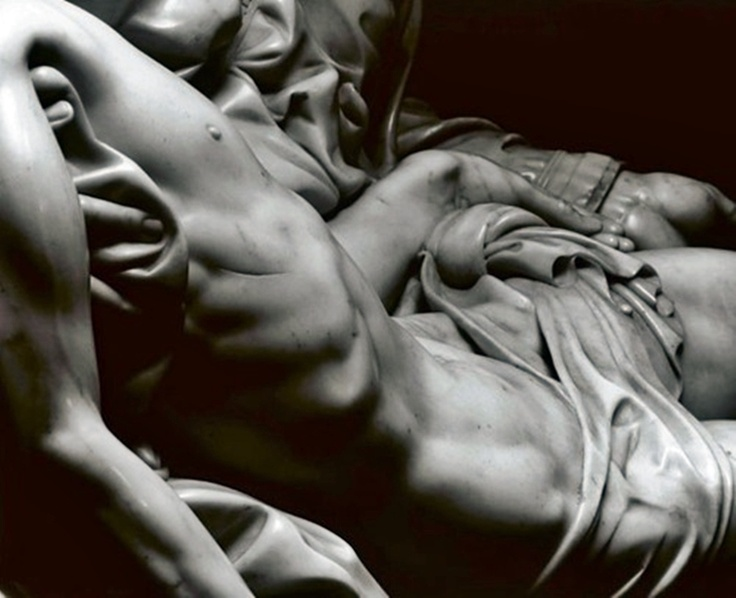
\includegraphics[height=0.35\linewidth ]{figure/Introduction/Mich.jpg}
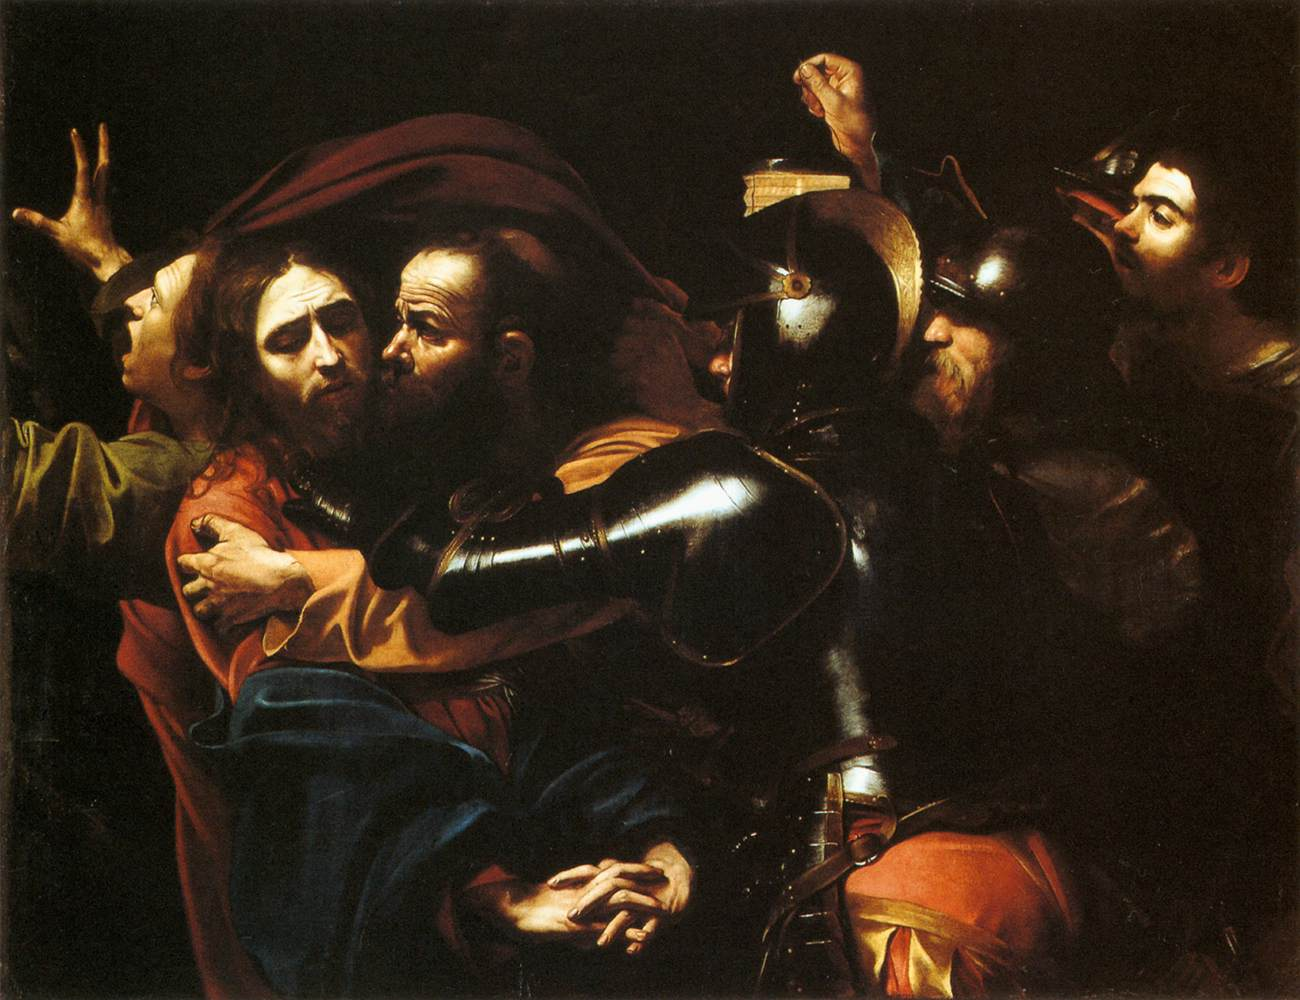
\includegraphics[height=0.35\linewidth ]{figure/Introduction/Caravaggio.jpg}
\caption{Michelangelo and Caravaggio}
\end{figure}

Similar challenges have master builders through time been facing. Creating master pieces that should not only be pleasing but also functional and obey the laws of physics. With task of reaching the heavens and creating light that should resemble the brace of god itself. 

\begin{figure}[H]
\centering
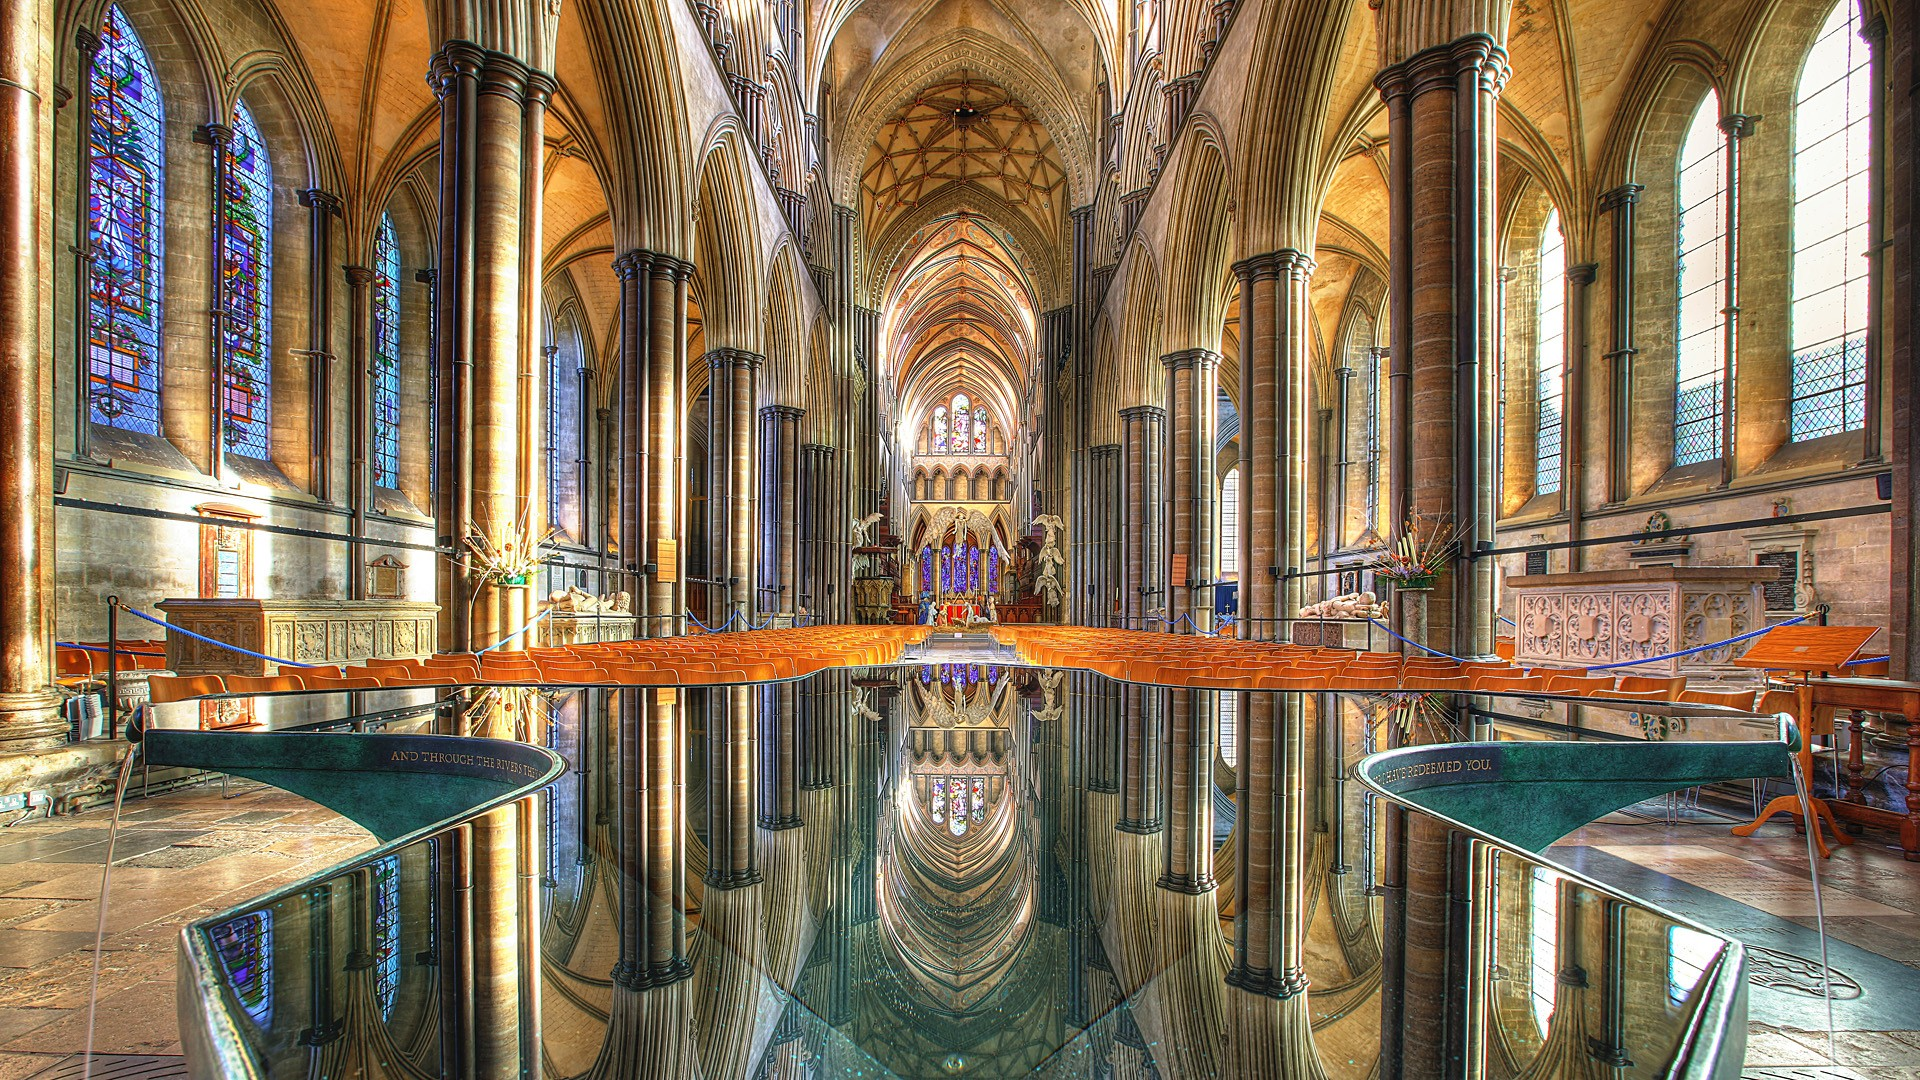
\includegraphics[width=0.9\linewidth ]{figure/Introduction/Salisbury.jpg}
\caption{Salisbury Church}
\end{figure}



A difficult assignment in many ways. Finding a pleasing and suitable form achieving what we today call equilibrium. Forms that should be able to discretize into elements of bricks or stones.
Approaching a building made by master builders and craftsmen you can be sure that lines are straight and curves circular. In a similar fashion as with Caravaggio you will notice that all bricks are not perfectly unit, sometimes deformed and distorted, even though straight using eye and spirit-level. Masters of illusion it might seem to be able to be able to use mortar and intuition to compensate faults in the material itself.

\begin{figure}[H]
\centering
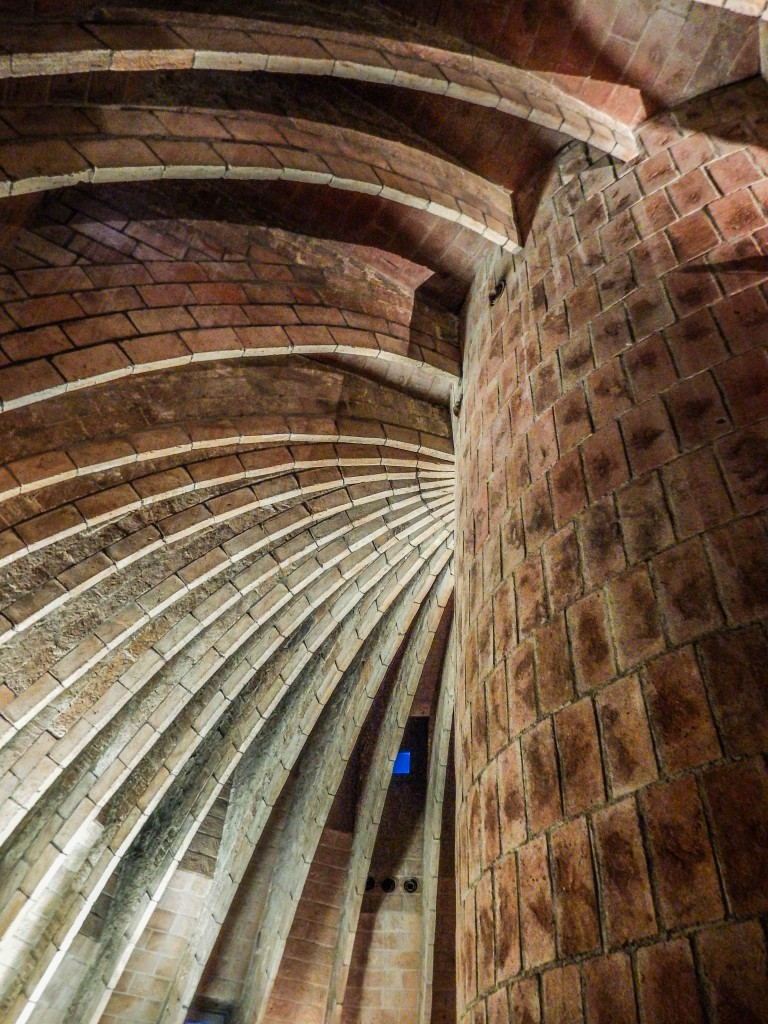
\includegraphics[height=0.5\linewidth ]{figure/Introduction/Casamila.jpg}
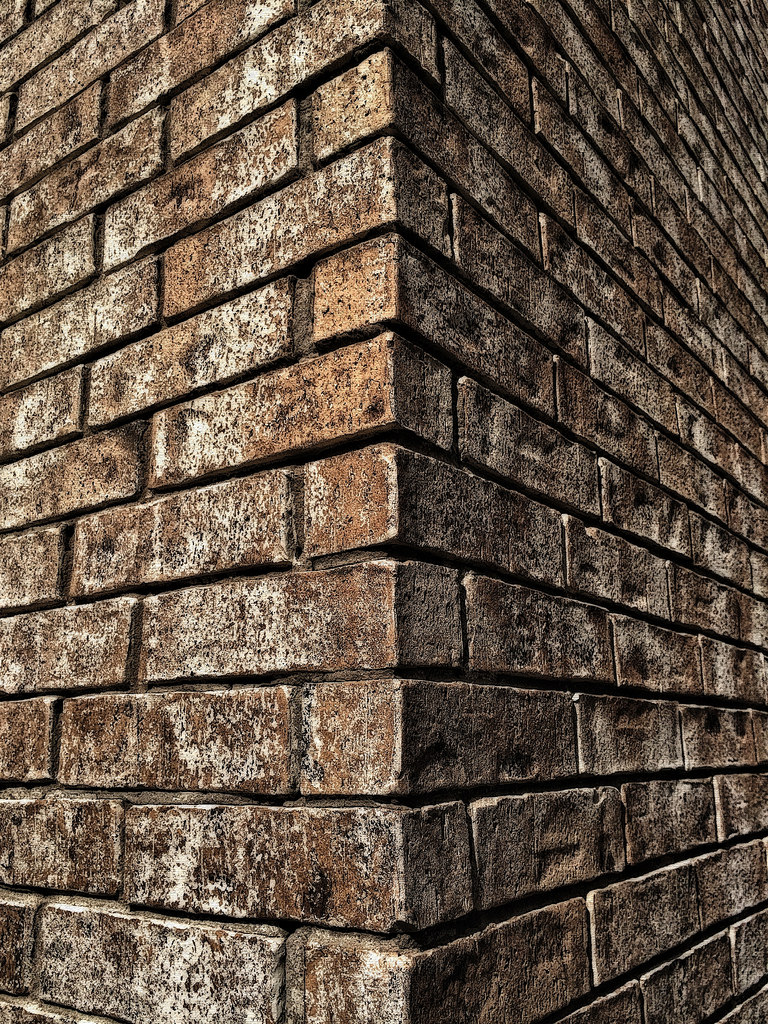
\includegraphics[height=0.5\linewidth ]{figure/Introduction/brickCorner.jpg}
\caption{Brickwall}
\end{figure}

The use of bricks and stone in modern time might not associated with elegance. More used as functional building material in residential buildings all over the world. The material that can take many shapes can also be considered as harsh if not handled with care. 
Still there are contemporary examples where Architects and Engineers have been inspired by history and achieved elegance, and even achieved new forms not possible to understand without todays computational methods.

\begin{figure}[H]
\centering
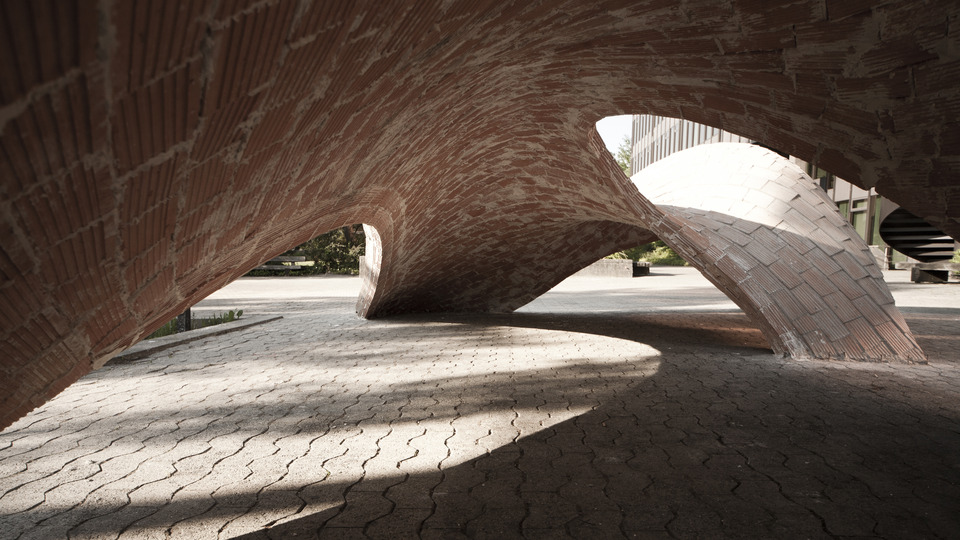
\includegraphics[width=0.9\linewidth ]{figure/Introduction/BlockVault.jpg}
\caption{http://light-earth.com/portfolio-items/mapunbubwe/}
\end{figure}

Something that blablabalblaba om the furturererer
Something that blablabalblaba om the furturererer
Something that blablabalblaba om the furturererer
Something that blablabalblaba om the furturerererSomething that blablabalblaba om the furturererer


\section{Context}
The following table presents an overview of the section levels that are used in this document. The number of levels that are numbered and included in the table of contents is set in the settings file \texttt{Settings.tex}. The levels are shown in Section \ref{Section_ref}.

\subsection{Shell Structures}

Vaults, cones and domes are the forms that are typically associated as shell structures. In architecture it is common for shell structures to consist of concrete bricks and stone. In modern times it can be reinforced using steel but historically it has been unreinforced. A shell could also be a car or plane body or a birds' eggs. Williams \\

Mentioning the most obvious shell form there are many different shapes of the shell, described by Heinz Isler.

\begin{figure}[H]
\centering
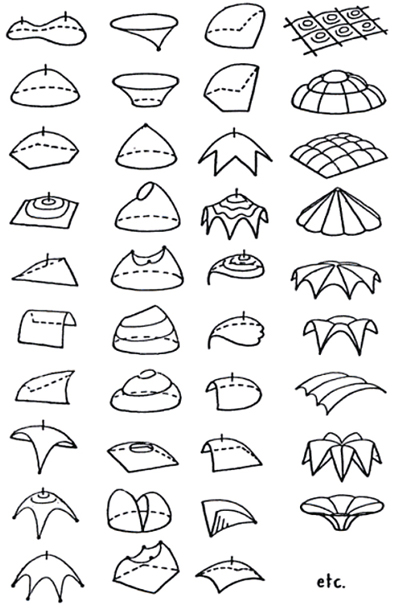
\includegraphics[width=0.6\linewidth ]{figure/Introduction/ShellDiagram.jpg}
\caption{Shell diagram over different types of shell by Heinz Isler}
\end{figure}

As Williams state there are many ways to describe a shell, but the most obvious definition might be through its geometry.

"A shell is a structure defined by a curved surface it is thin in the direction perpendicular to the surface, but there is no absolute rule as to how thin it has to be. It might be curved in two directions, like a dome or a cooling tower, or it may be cylindrical and only curve in one direction." Williams Architecture Shell.

In the book Shell Structure you can read this definition of a shell structure taking its.

"Shell Structures are constructed systems described by three-dimensional curved surfaces, in which one dimension is significantly smaller compared to the other two. They are form-passive and resist external loads predominately through membrane stresses." Introduction 

A form-passive structure meaning that you do not experience much degrees of change of shape or form. Where a form-passive would break under high deflection a form-active can adapt to a new equilibrium state like cables or membrane structures. Source needed? 
Membrane stress and membrane structures should not be mixed up. Membrane condition is when the forces are mainly carried in the plane of the shell surface. Membrane stresses can be in compression, tension or a combination of them both. \\



In the book Shell structures for Architecture optimisation it distinguish between three types of geometries for Shell Structures, and defined as following.

\begin{itemize}
\item Freeform, free-curved or sculptural shells are generated without taking into consideration structural performance.  
\item Mathematical, geometrical or analytical shells are directly described by analytical functions.These functions are of then chosen for their convenience in performing further analytical calculations and their ability to describe a shell's shape for fabrication purposes.
\item Form Found shells include natural, hanging shapes assosiated with funicular structures of Antoni Gaudi, Frei Otto and Heinz Isler, but also "strained" gridshells tat feautre bending stresses. Their final shape is a result of attaining a state of static equilibrium.
\end{itemize}

\subsubsection{Gridshells}


"A gridshell is essentially a  shell with its structure concentrated into individual members in a relatively fine grid compared to the overall dimensions of the structure. The members may be short and only pass from node to node, or they may be continuous, crossing each other at the nodes. The grid may have more than one layer, but overall thickness of the shell is small compared to the overall span" p89

Common materials for gridshells have been timber and steel. Examples of timber gridshells are Mannheim Multihalle, by Frei Otto, Downland Gridshell and 

\begin{figure}[H]
\centering
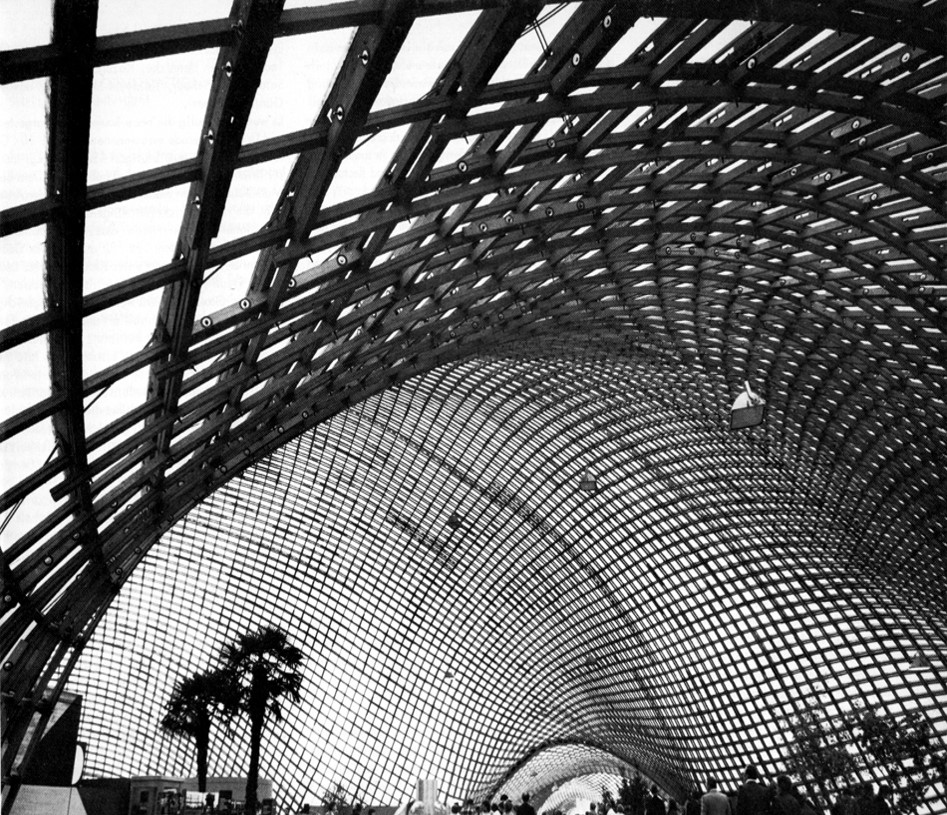
\includegraphics[width=0.3\linewidth ]{figure/Introduction/DownlandC.jpg}
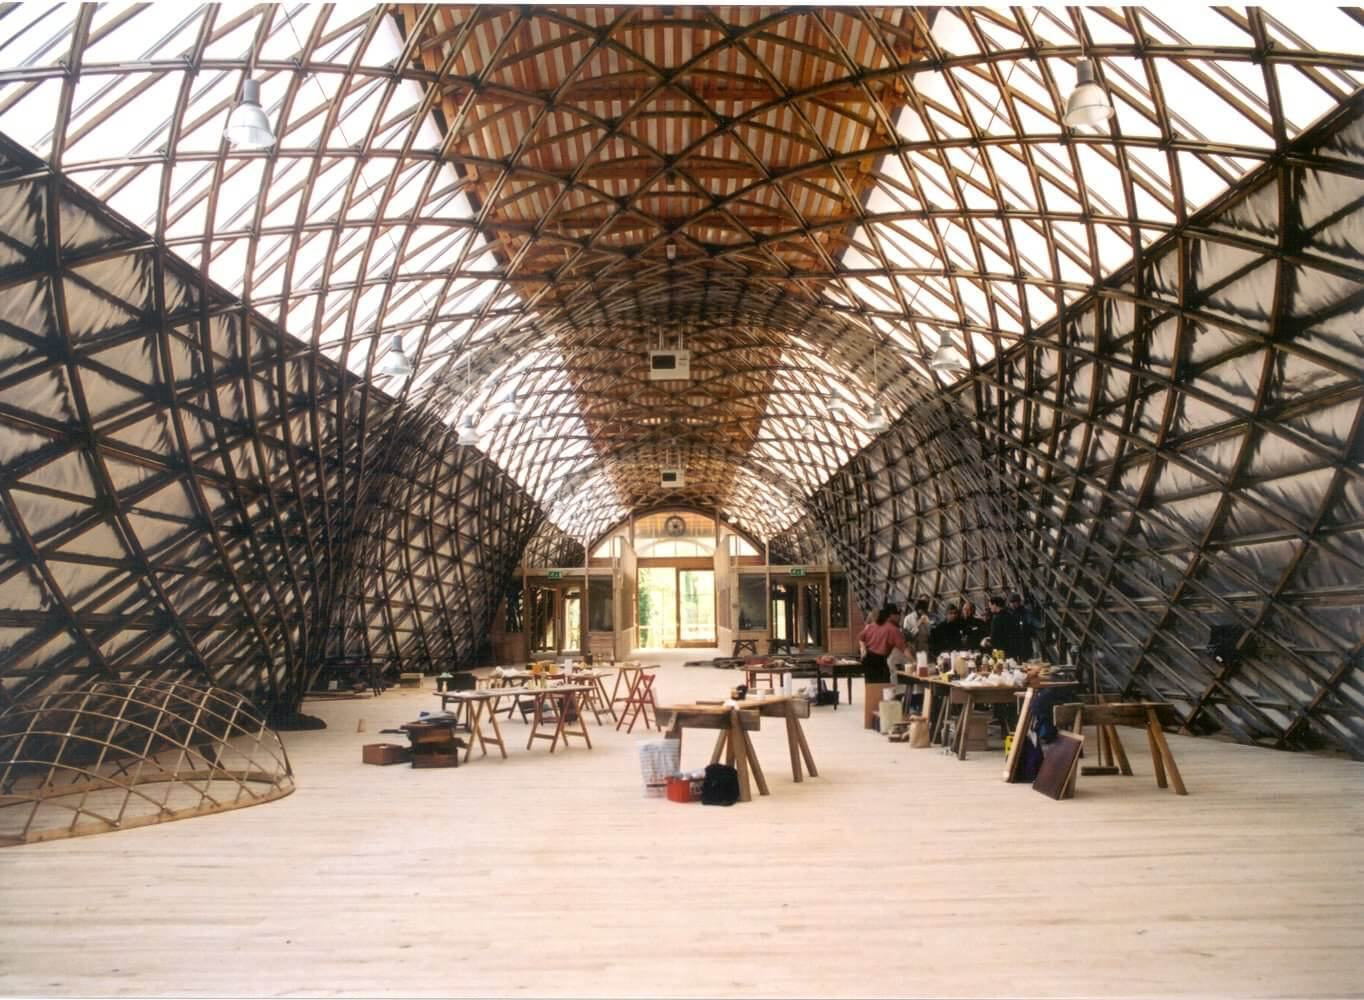
\includegraphics[width=0.3\linewidth ]{figure/Introduction/Downland.jpg}
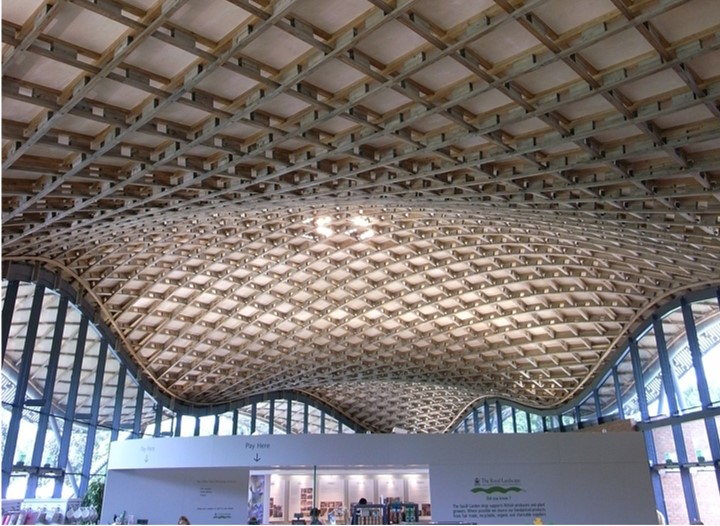
\includegraphics[width=0.3\linewidth ]{figure/Introduction/Savill.jpg}
\caption{Multihalle and Downland Gridshell}
\end{figure}

\begin{figure}[H]
\centering
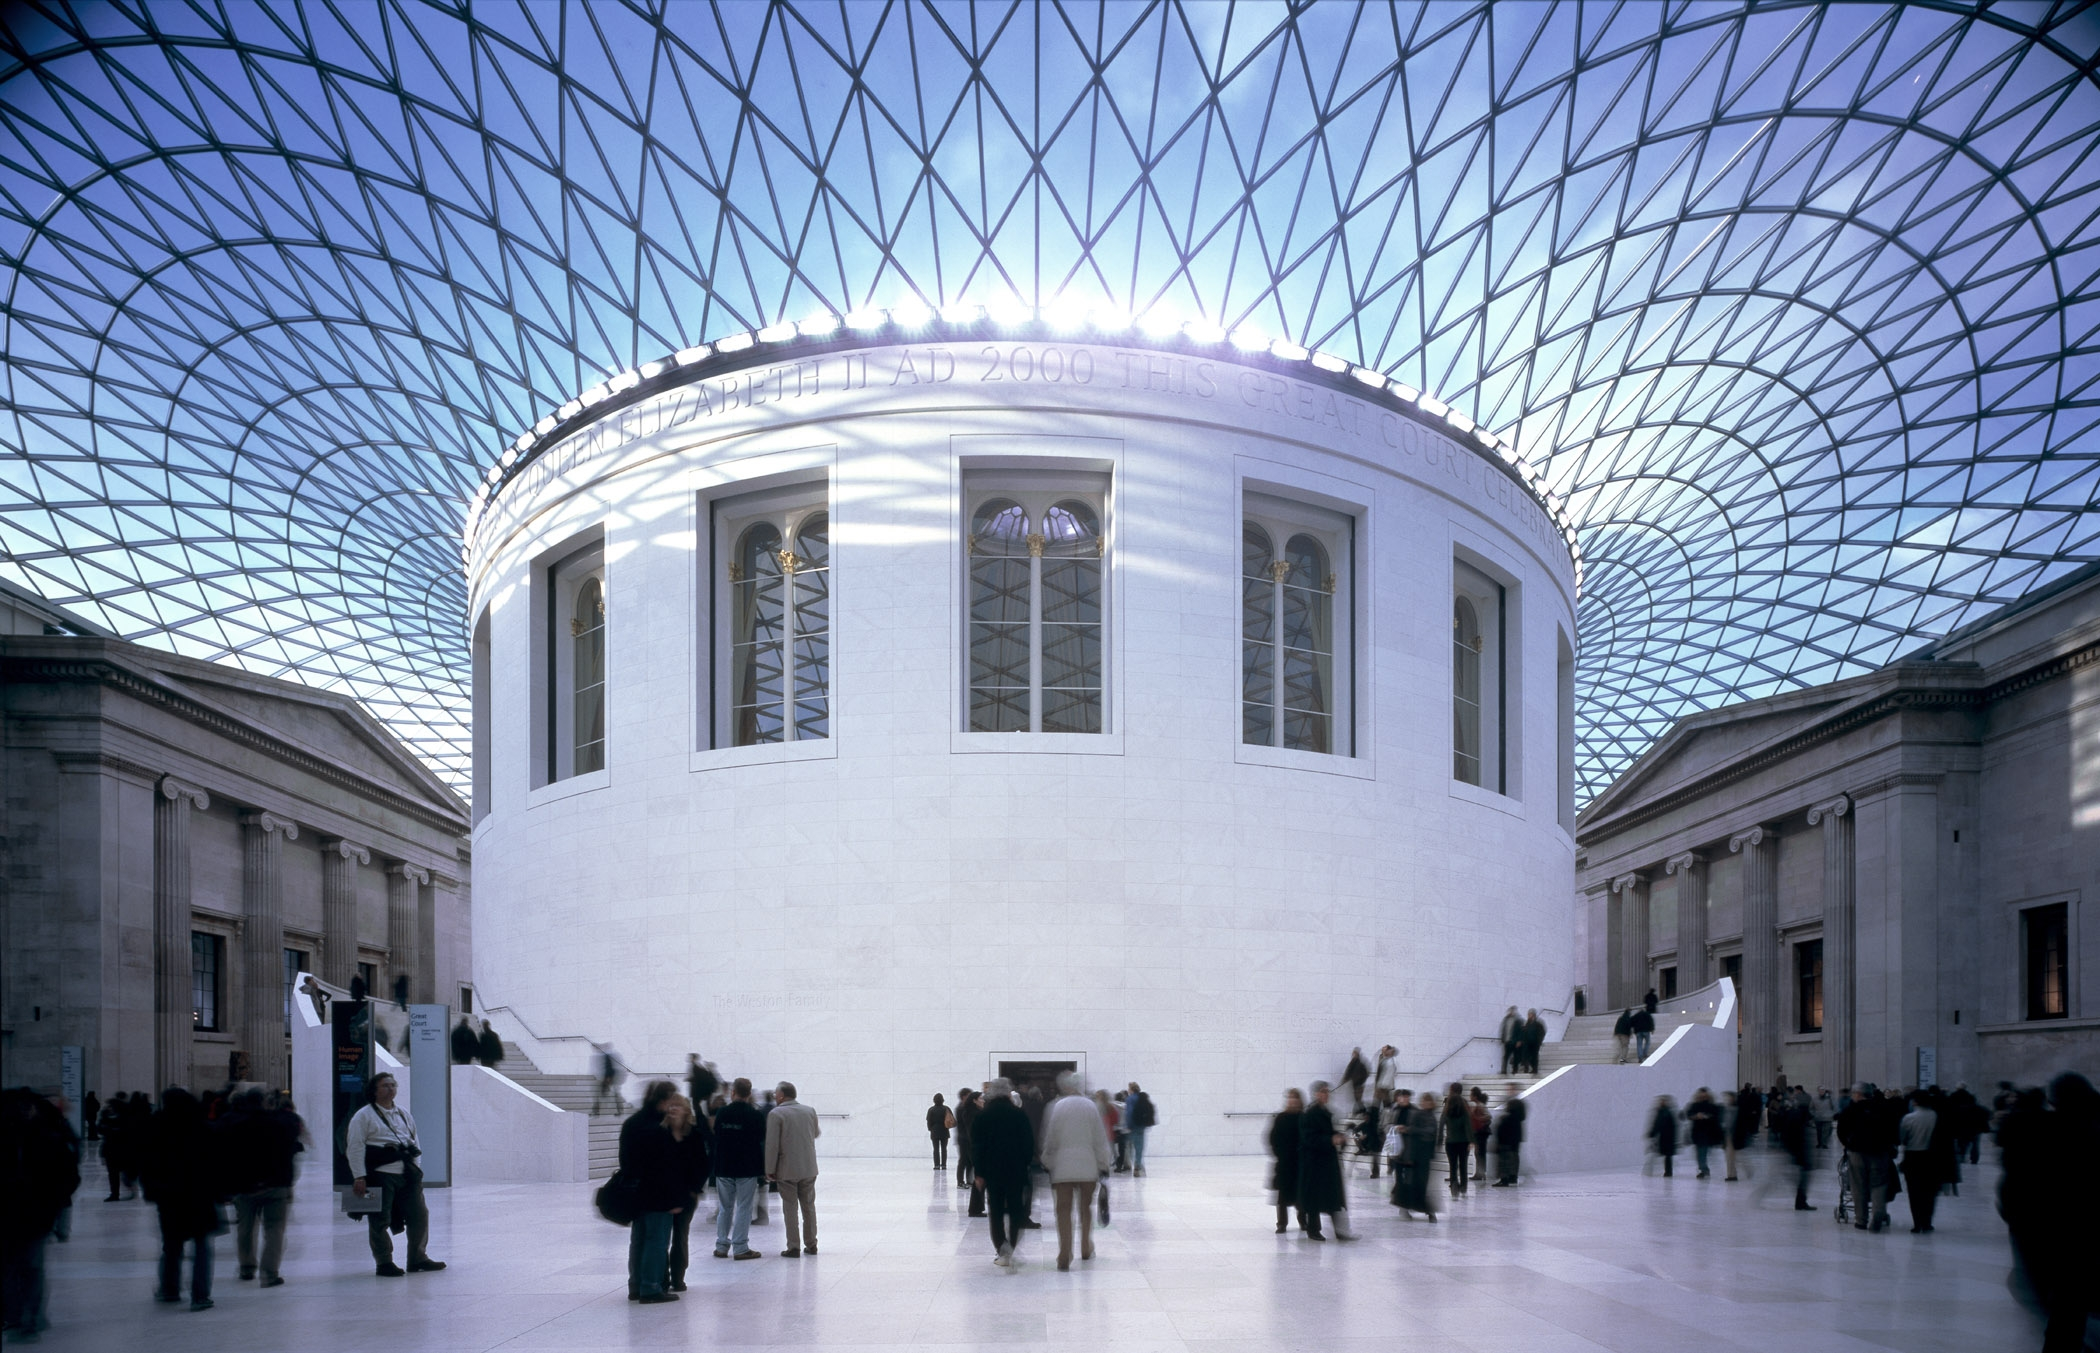
\includegraphics[width=0.9\linewidth ]{figure/Introduction/TheGreatCourt.jpg}
\caption{British Museum court roof}
\end{figure}


\subsection{Masonry}

Masonry can be read as the art and craft of building in stone, clay, brick or concrete block in Encyclopedia of Britannica. These elements can be of various shapes and configured and placed on one another to form a stable structure. It can be a collection of dry elements, meaning no mortar to connect the elements, or using some type of mortar to bind the pieces together. 



\subsubsection{Early history of Masonry}
Masonry is a very old tradition in the history of mankind. One of the oldest findings of masonry is  chambered tombs that is  dry-wall masonry(stones laid without mortar) with corbels roofs constructed in Spain and France, dated to ca 4200 BCE. 

\begin{figure}[H]
\centering
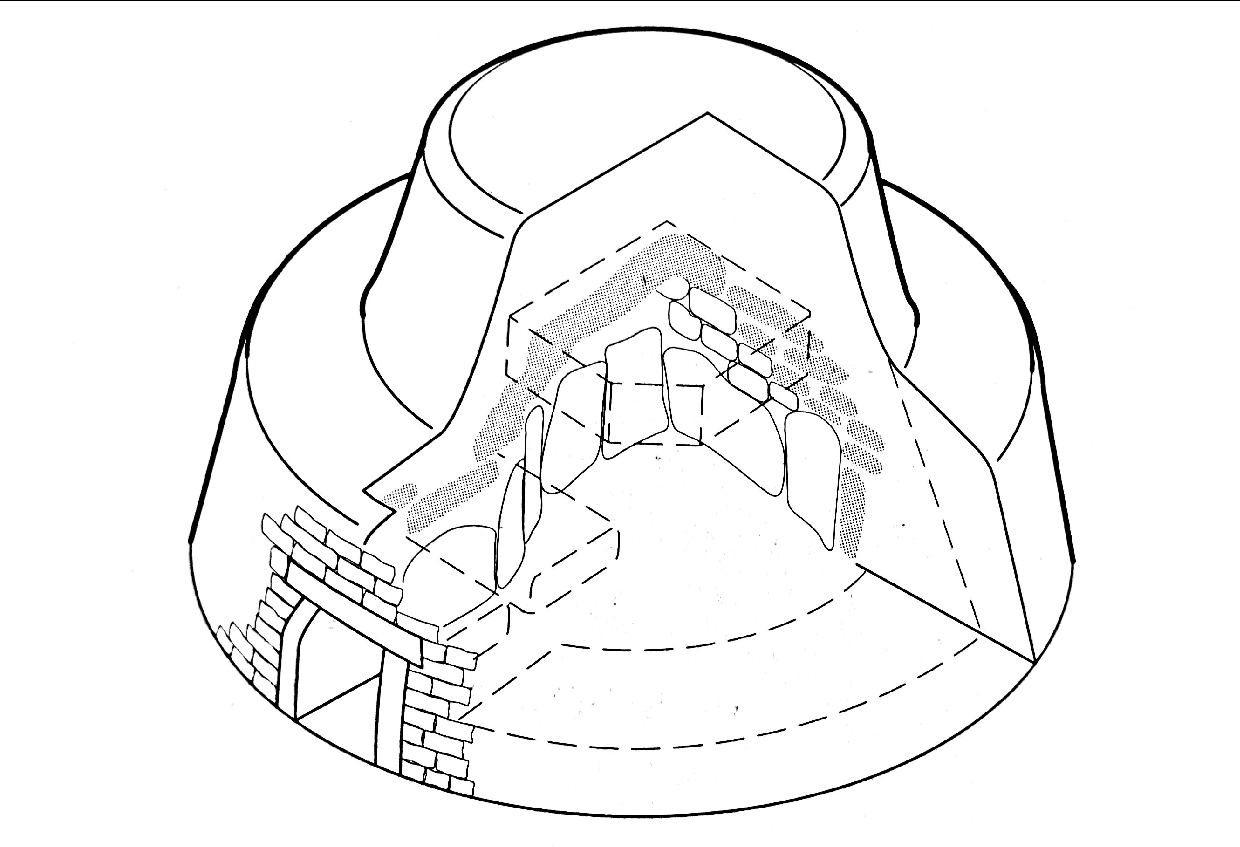
\includegraphics[height=0.3\linewidth ]{figure/Introduction/oldMasonry2.pdf}
\caption{Megalith tomb, Er-Mané,Carnac,Brittany,France,ca 4200 BCE}
\end{figure}

Later, about 3000 BCE in Mesopotamia, the first fired bricks appeared, which was a development from the sun dried mud brick used even earlier.
Egypt also built it cities with using of mud bricks, but they unlike Mesopotamia or the Indus valley, had excellent deposits of stone exposed above ground; limestone, sandstone, and granite were all available.
Therefore a new technology of cut-stone construction emerged in the temples and pyramids of the 4th dynasty (c. 2575–c. 2465 bce).(britannia, building construction) 

\begin{figure}[H]
\centering
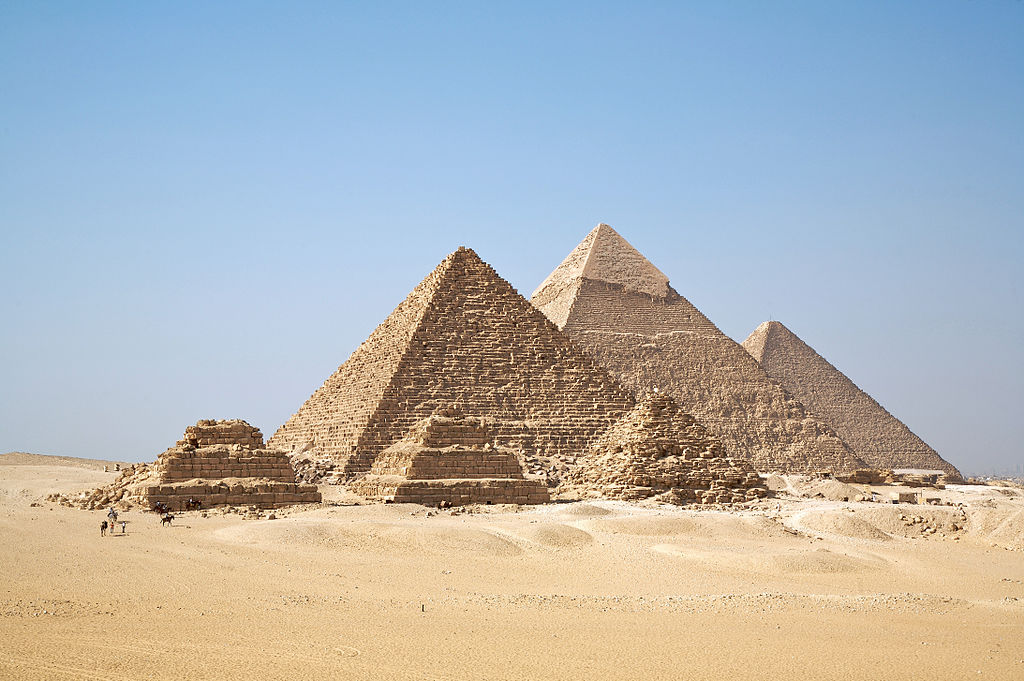
\includegraphics[width=0.5\linewidth ]{figure/Introduction/GizahPyramids.jpg}
\caption{Pyramids of Gizah, ca 2500 BCE,wikipedia}
\end{figure}

The use of concrete was invented by the Romans, who also refined the use of bricks and stone. The most famous example of concrete structures is Pantheon in Rome, which is a dome made of concrete blocks.
\begin{figure}[H]
\centering
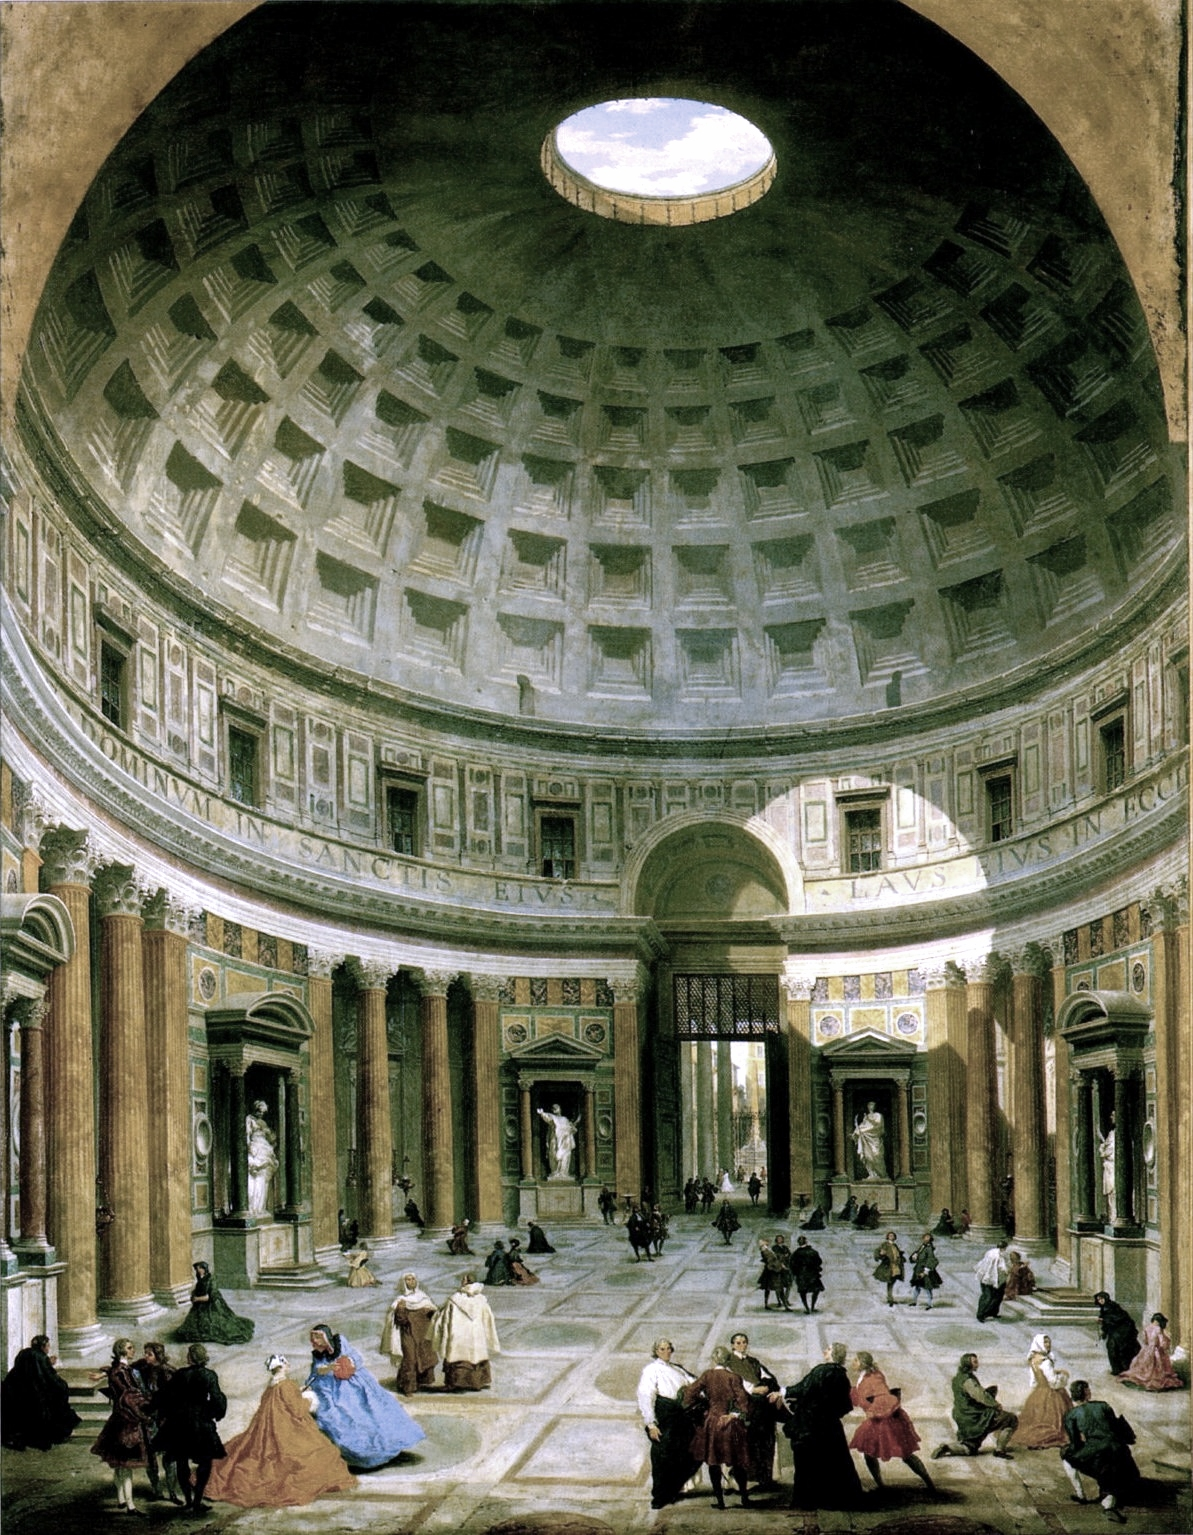
\includegraphics[width=0.5\linewidth ]{figure/Introduction/Pantheon.jpg}
\caption{Pantheon, Wikipedia}
\end{figure}


\subsubsection{Modern Masonry Shells in Architecture}

As mentioned section about shells it is a structural element defined by a curved surface that is thin in the direction of the normal. Early, if not the first, to master shell structures  was the Romans. Pantheon, built in early 2nd Century, is a great example of the Roman understanding of geometry and shells. It is built of concrete elements and with an oculus as a light source. The grid structure might be just decorative but it is possible to read as an understanding of that forces can be handled in both radial and angular direction of the dome.

\begin{figure}[H]
\centering
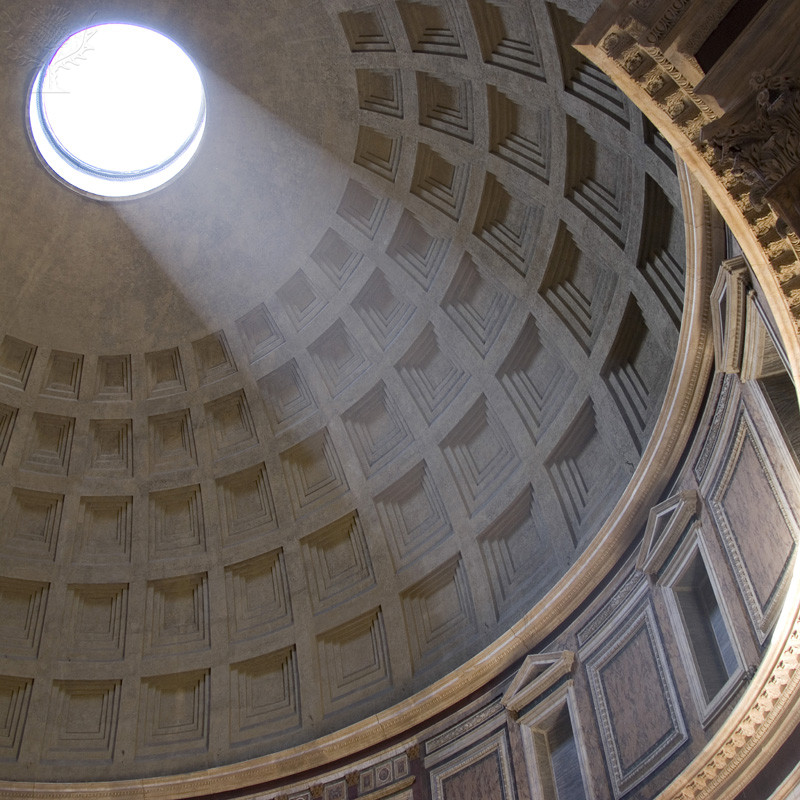
\includegraphics[width=0.9\linewidth ]{figure/Introduction/Pantheon1.jpg}
\caption{Britannica image}
\end{figure}


The structures of vaults and domes has a strong position in most historic description of Architecture. Two names that stand out in modern time architecture in this genre are \textit{Rafael Guastavino} and \textit{Eladio Dieste}. They are seen as the main contributors to revolutionise the structural arts of masonry shells and take it into the modern era. 
"Until late in the nineteenth century, masonry vaulting was shaped and proportioned by guesswork or rules of thumb. As a consequence, vaults based on the European or Middle Eastern precedents tended to be not only thick but also heavy and expensive. Catalan vaults were much thinner but were also designed by wholly intuitive methods."
Instead of rely on intuition Guastavino used \textit{graphic statics} which was a relatively new method at the time to describe and understand force patterns of structures. Graphic statics made it possible to visualise the optimal shape of vaults and trusses. This in combination with the technique of catalan vaults made it possible to construct very slender structures. "Although Guastavino patented techniques for both reinforcing and post-tensioning, most of his roofs were constructed of unreinforced masonry"





 John Oschendorf describs the legacy of the Guastavino Company \textit{"With complex three dimensional vaults, supported by carefully placed stiffening walls, flying buttresses, and tension ties, the Guastavinos worked as master masons in the modern era"} 

\begin{figure}[H]
\centering
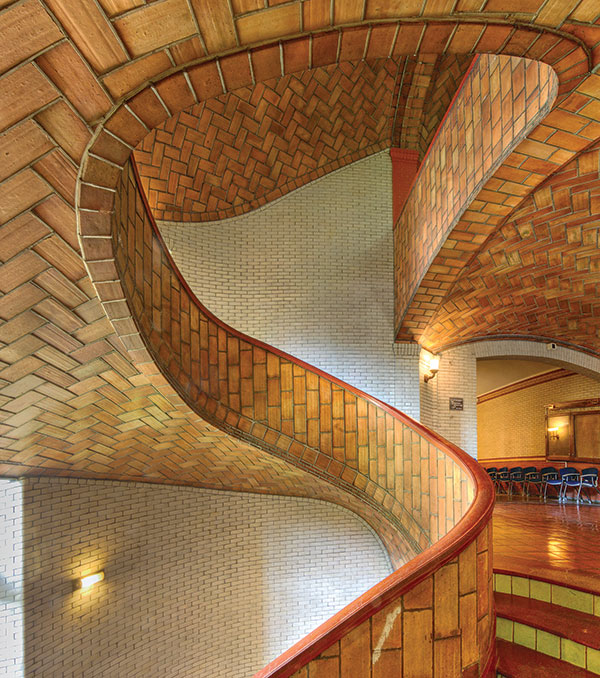
\includegraphics[height=0.4\linewidth ]{figure/Introduction/GuastovinoStair.jpg}
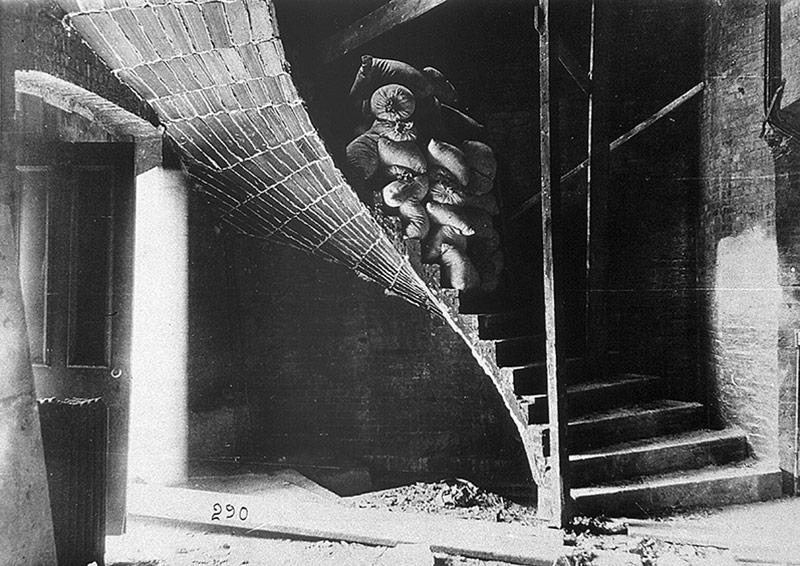
\includegraphics[height=0.4\linewidth ]{figure/Introduction/GuastavinoStair2.jpg}
\caption{Tile vaulted staircase of Baker Hall, Carnegie Mellon University, Pittsburgh, 1914. Courtesy of Michael Freeman.}
\end{figure}

Dieste did in comparison to Guastavino use formwork during construction and worked only with steel reinforced and often post tensioned structures.Instead of using Graphic Statics Dieste used numerical methods to design his structures. "Dieste’s building structures fall into four general categories, none of which was feasible in Guastavino’s time."

\begin{itemize}

\item Gaussian Vaults
\item Self supporting shells
\item Folded structures
\item Ruled surfaces
\end{itemize}

\begin{figure}[H]
\centering
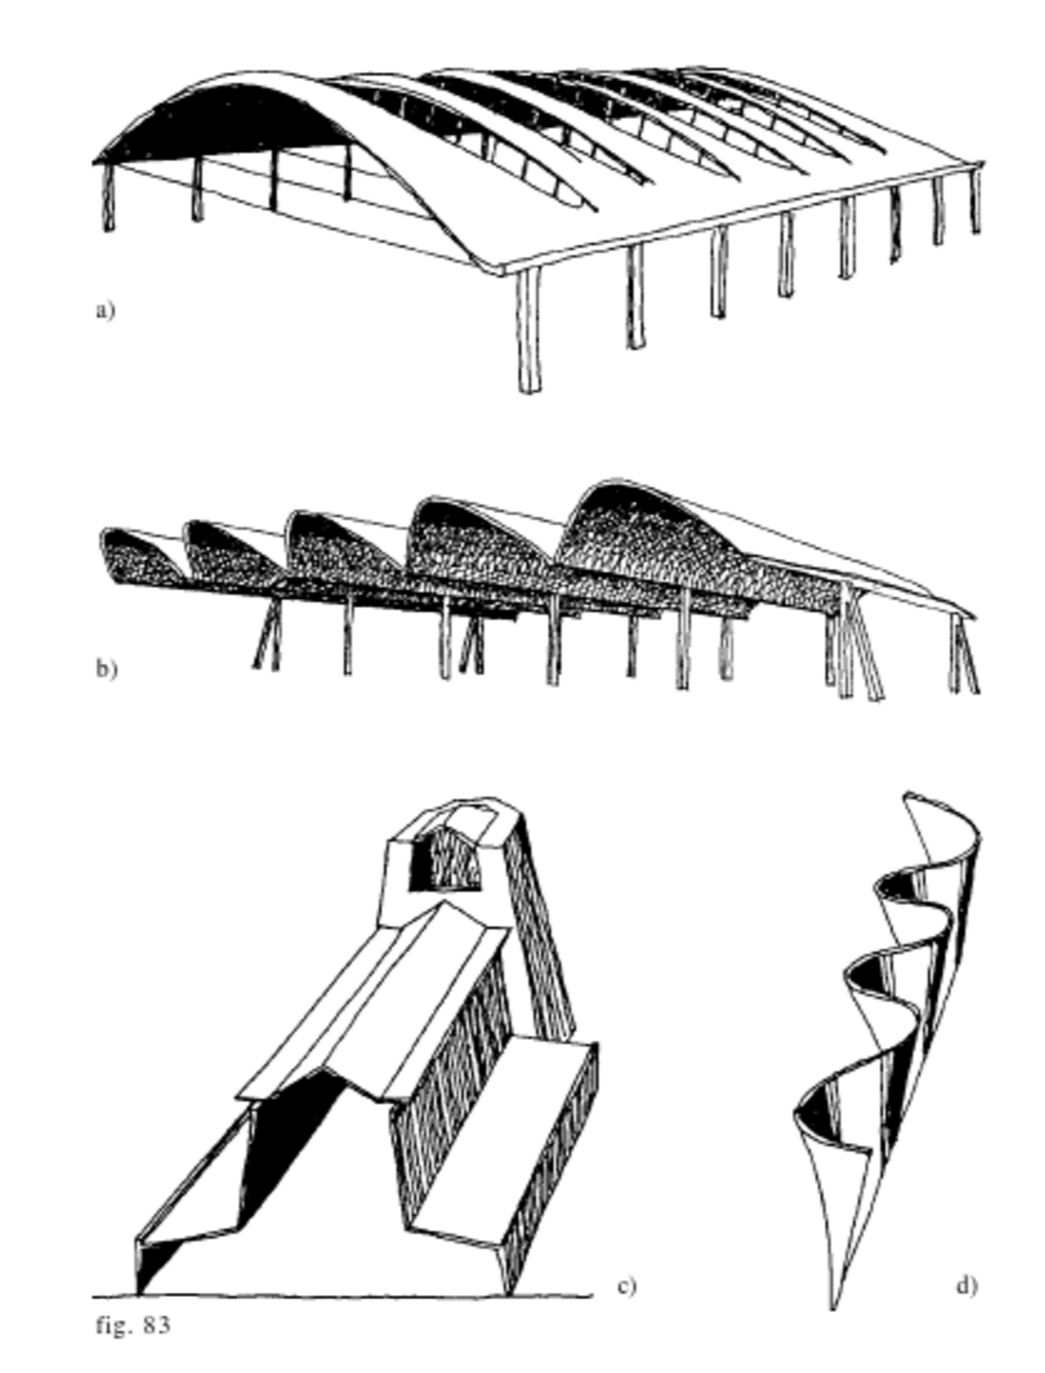
\includegraphics[width=0.4\linewidth ]{figure/Introduction/DiesteFour.JPG}
\caption{The four categories of Dieste Eladio Dieste: innovation in structural art}
\end{figure}

"There were others as well who built with reinforced brickwork, but two things set Dieste’s work above the rest. One is his unmatched use of masonry in structures subject to bending, such as cantilevered barrel shells, tanks under hydrostatic pressure, and folded plates. The other is the power and poetry of his masonry architecture."


\begin{figure}[H]
\centering
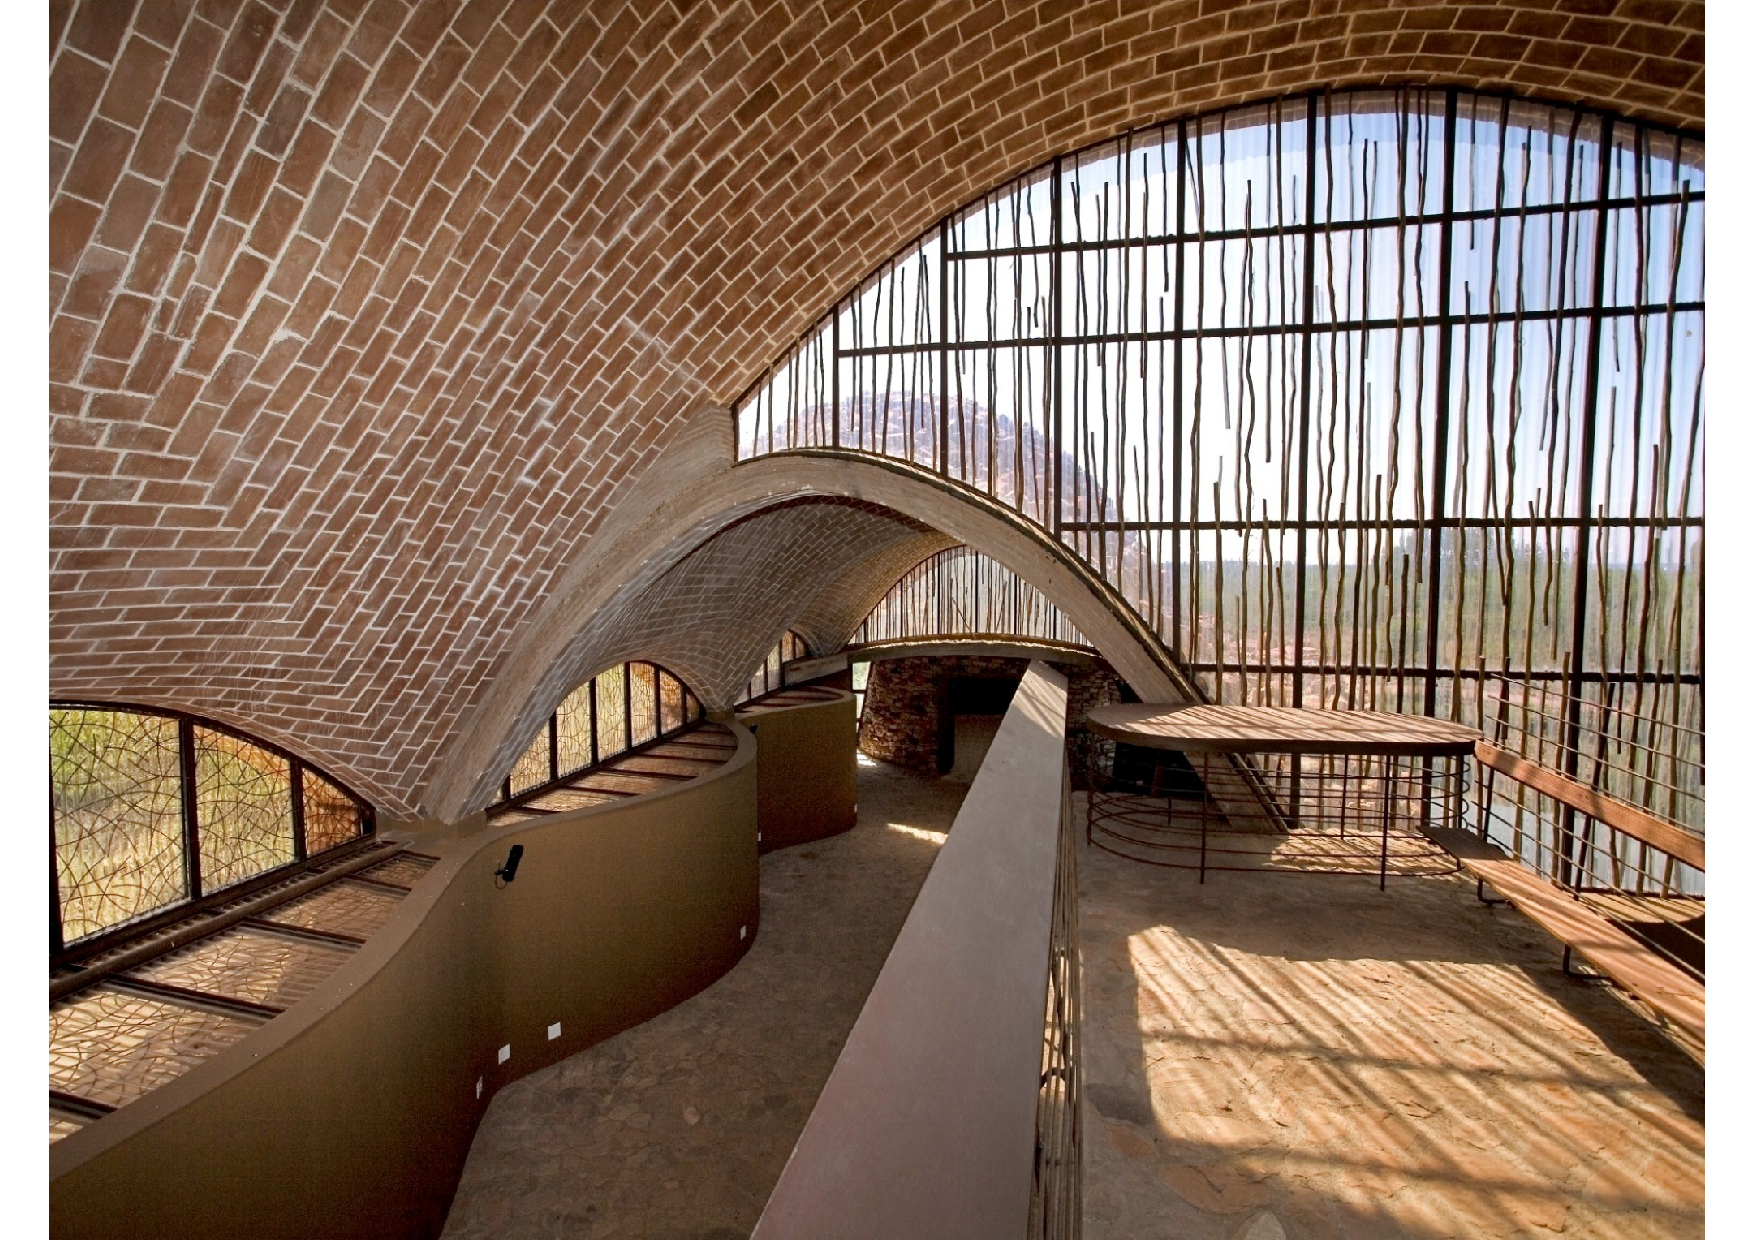
\includegraphics[width=0.9\linewidth ]{figure/Introduction/Vault_Contemporary.pdf}
\caption{http://light-earth.com/portfolio-items/mapunbubwe/}
\end{figure}


\begin{figure}[H]
\centering
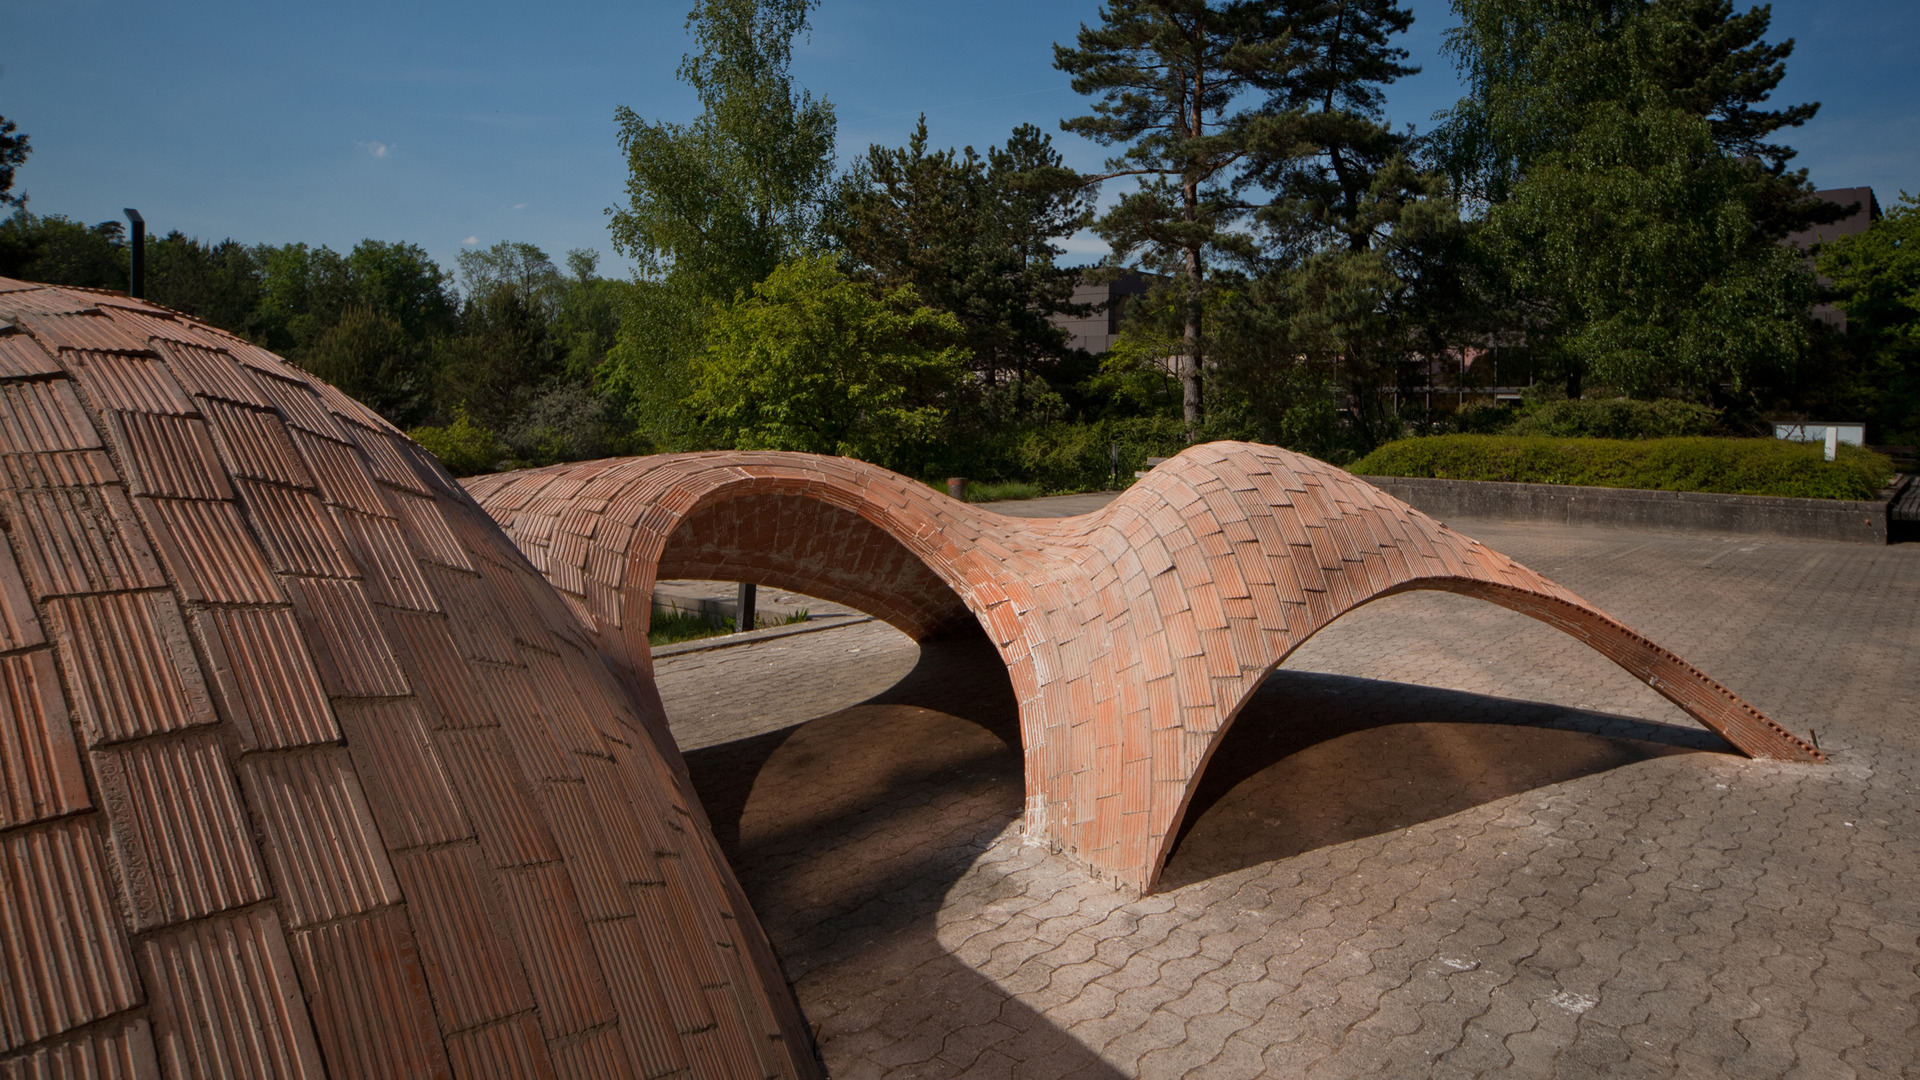
\includegraphics[width=0.9\linewidth ]{figure/Introduction/Block_Vault.jpg}
\caption{Surface and contour plots showing $z(x,y)=\sin(x+y)\cos(2x)$.}
\end{figure}

\subsection{Geometrical Challenges}

Travelling has been an important part of the human history and it almost feels like a part of our DNA to discover new horizons. Therefore one of the most common geometrical queries of today and the past might be \textit{"I want to go from A to B and how do I know where to go and which of all options are the best"}. An essential part in our lives is to relate our position and relating objects in space based on maps. The question is how to transform something three dimensional into two dimensions such as paper, this is known to be an impossible problem to solve. A solution to this problem was discovered by  \textit{Gerardus Mercator} in 1569, a so called \textit{Mercator Projection}. This is basically a method to project a sphere onto a cylinder that can be unrolled to a plane. This is of course not true since the projection becomes different depending on your distance to the equator, and the poles can not even be projected. 550 years later this method is still used in applications such as \textit{Google Maps}. So every time we search and evaluate our surroundings on Google Maps we actually are demanding a very difficult geometrical query. 

\begin{figure}[H]
\centering
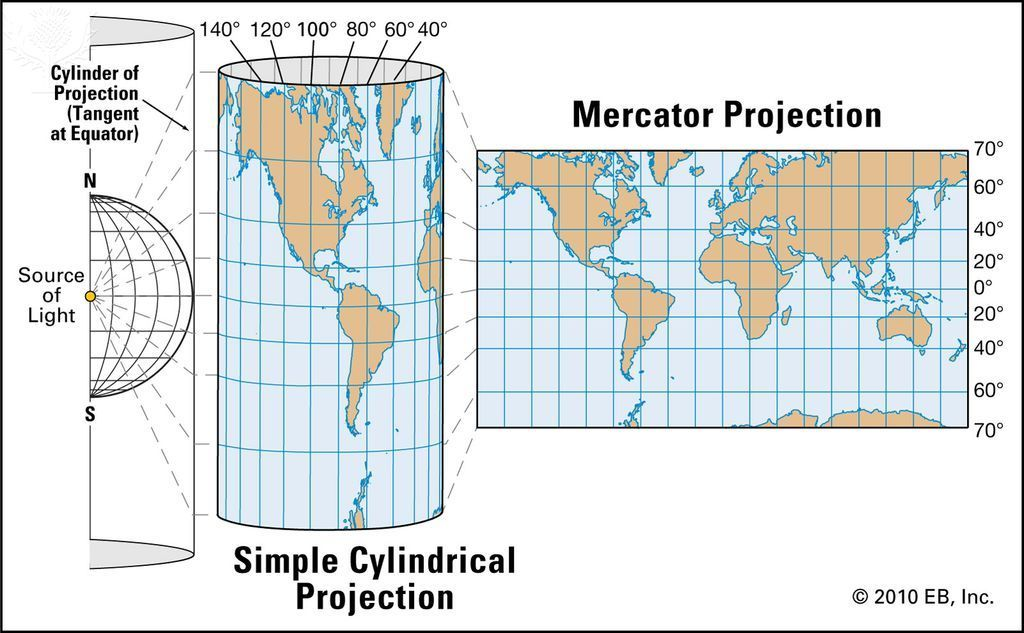
\includegraphics[width=0.9\linewidth ]{figure/Introduction/Mercator.jpg}

\caption{The length of the curve is the same regardless of coordinate system.}
\end{figure}

More hands on puzzles might be looking at a football or the jeans you are wearing and the cutting pattern made by the designer. Our the other way around how would you do a cutting pattern to something as irregular as the human body. The football is definitely simpler but still not easy with its mix of pentagons and hexagons, why cant you just make rectangle or squares?

\begin{figure}[H]
\centering
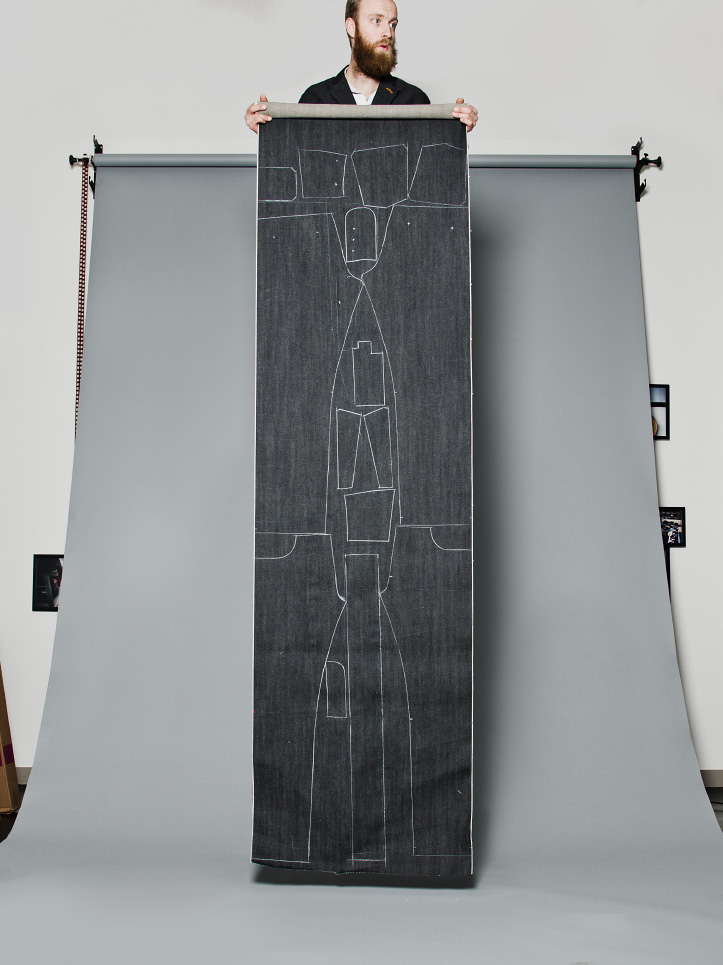
\includegraphics[height=0.4\linewidth ]{figure/Introduction/Jeans.jpg}
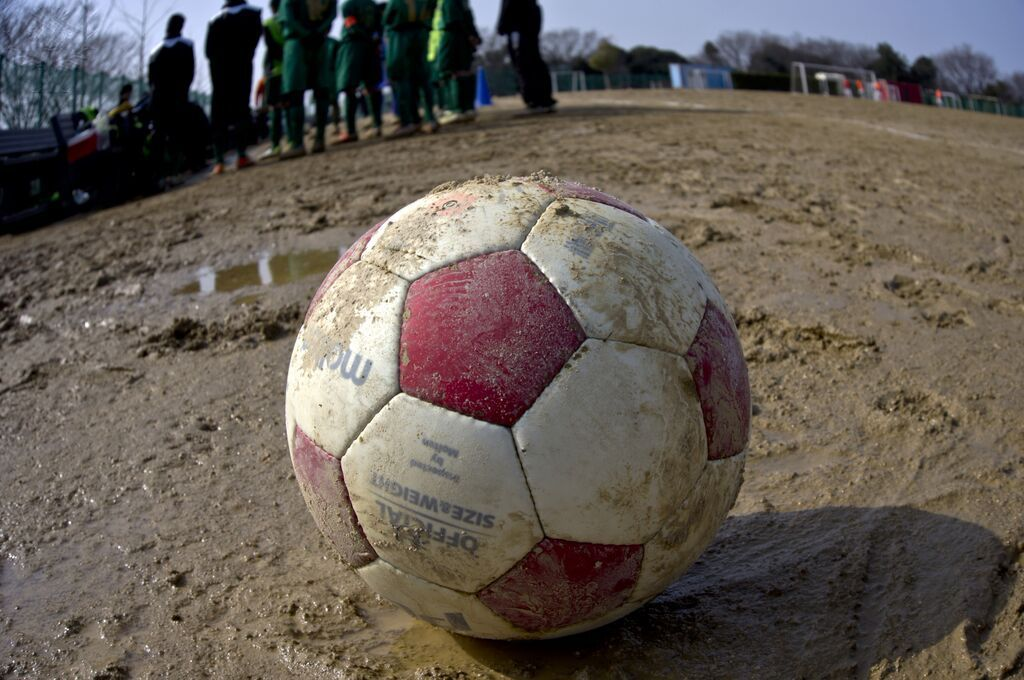
\includegraphics[height=0.4\linewidth ]{figure/Introduction/football.jpg}
\caption{The length of the curve is the same regardless of coordinate system.}
\end{figure}

It might sound silly but these are problems for Architects and Engineers. How do we discretize a geometrical shape into building elements. We often would like to make a pattern in 2D and make it 3D for aesthetic and economical reasons, this way we could build everything in a one sized panel for instance. As for Mercator it is just not possible in theory to a direct transformation without distorting the image. The initially same sized squares become sewed and in different sizes.
Two ways to tackle this is to use a module like brick where you can work with tolerances using mortar and accept a deviation from the theoretical shape. Another way is to to work closely with the mathematical discretization of the global form and the production of the local elements and only allow small deviations. \\
Tensile structures are like the jeans you wear, it needs to be designed and cut correctly to look nice, and depending on the geometry it can be more or less complicated. Pioneer in this field is Frei Otto who started to eleboarate with textile and membrane structures. Below is an example from a contemporary project called Green Void by LAVA in Sydney.

\begin{figure}[H]
\centering
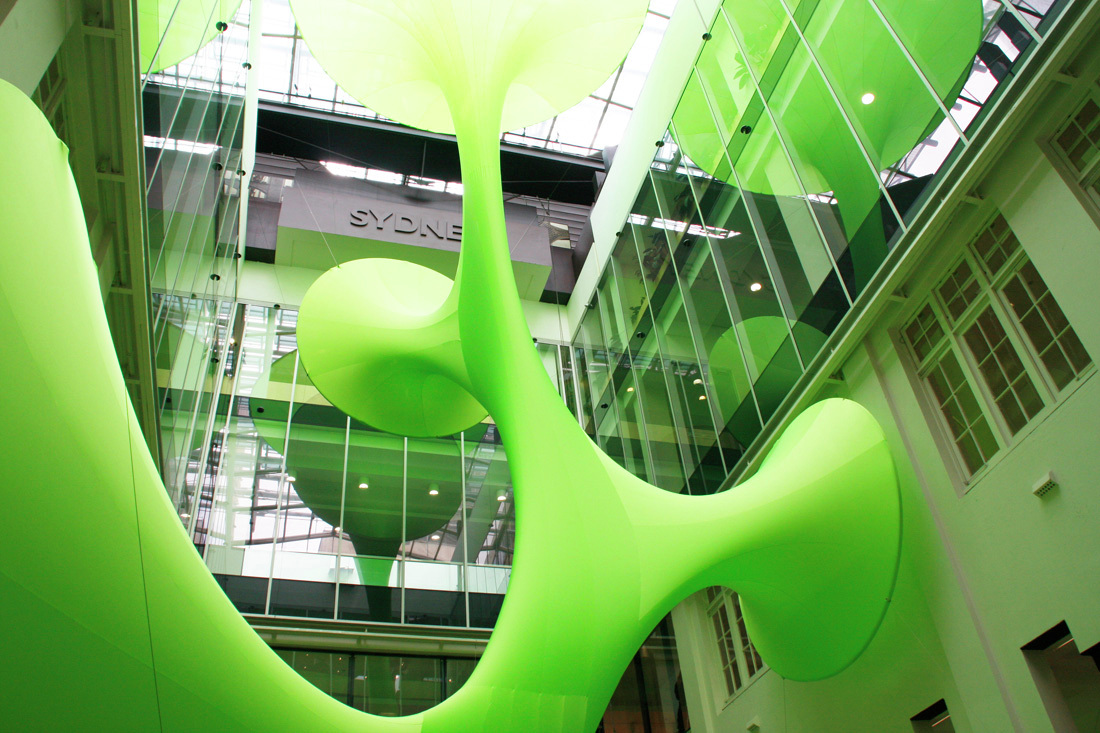
\includegraphics[height=0.30\linewidth ]{figure/Introduction/GreenVoid2.jpg}
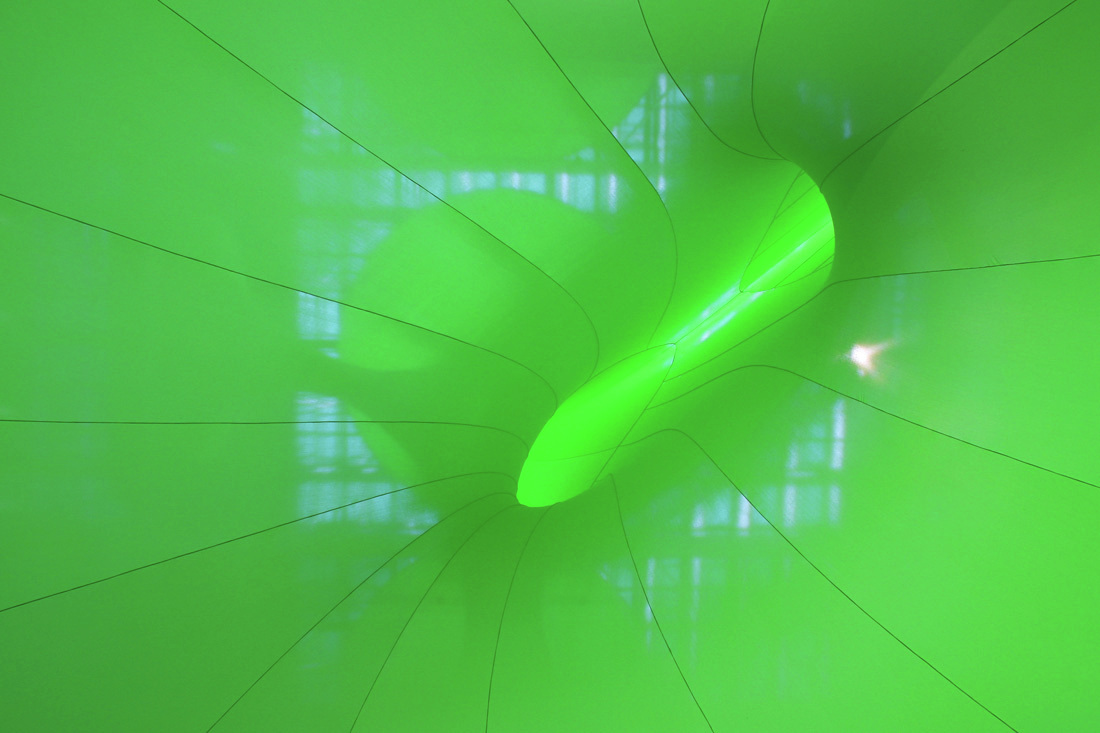
\includegraphics[height=0.30\linewidth ]{figure/Introduction/GreenVoid1.jpg}
\caption{The length of the curve is the same regardless of coordinate system.}
\end{figure}

The shape of the the ball and its discretization have some resemblance with the works of Buckminster Fuller which is especially known for developing the so-called geodesic dome. Ture Wester describes the generation of these structures but call it \textit{systematic triangulation of the regular polyhedra}. It is based on a subdivison of the icoshedra which is a platonic body.

\begin{figure}[H]
\centering
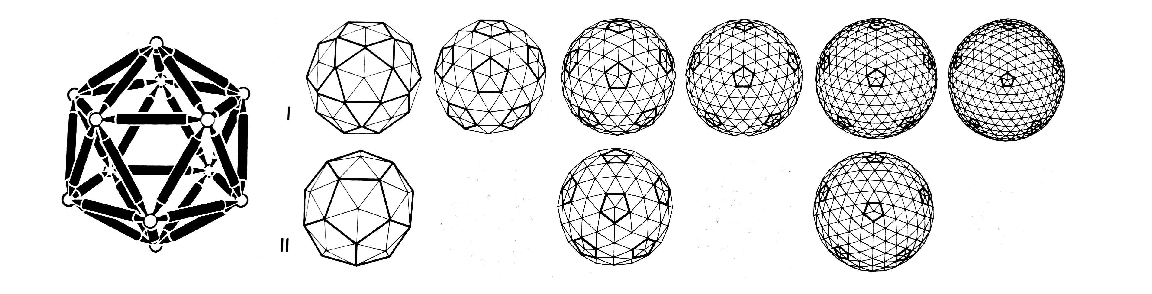
\includegraphics[height=0.25\linewidth ]{figure/Introduction/TureW6Mod.pdf}
\caption{The length of the curve is the same regardless of coordinate system.}
\end{figure}

\begin{figure}[H]
\centering
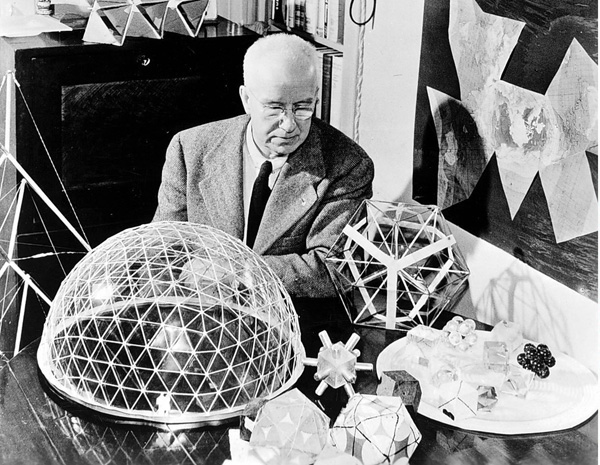
\includegraphics[height=0.30\linewidth ]{figure/Introduction/fuller3.jpg}
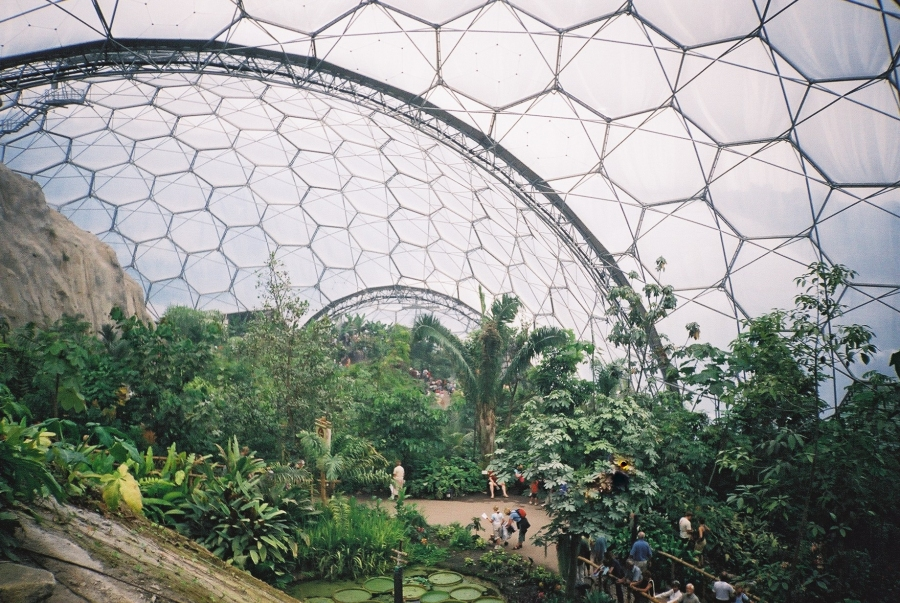
\includegraphics[height=0.30\linewidth ]{figure/Introduction/Eden.jpg}
\caption{The length of the curve is the same regardless of coordinate system.}
\end{figure}

\subsubsection{Stereotomy }
  
Stereotomy is defined as "the science or art of cutting solids into certain figures or sections". It includes, and the term is sometimes used as a synonymous with, the art of cutting stones for masonry shells. From Notes of Stereotomy.

\begin{figure}[H]
\centering
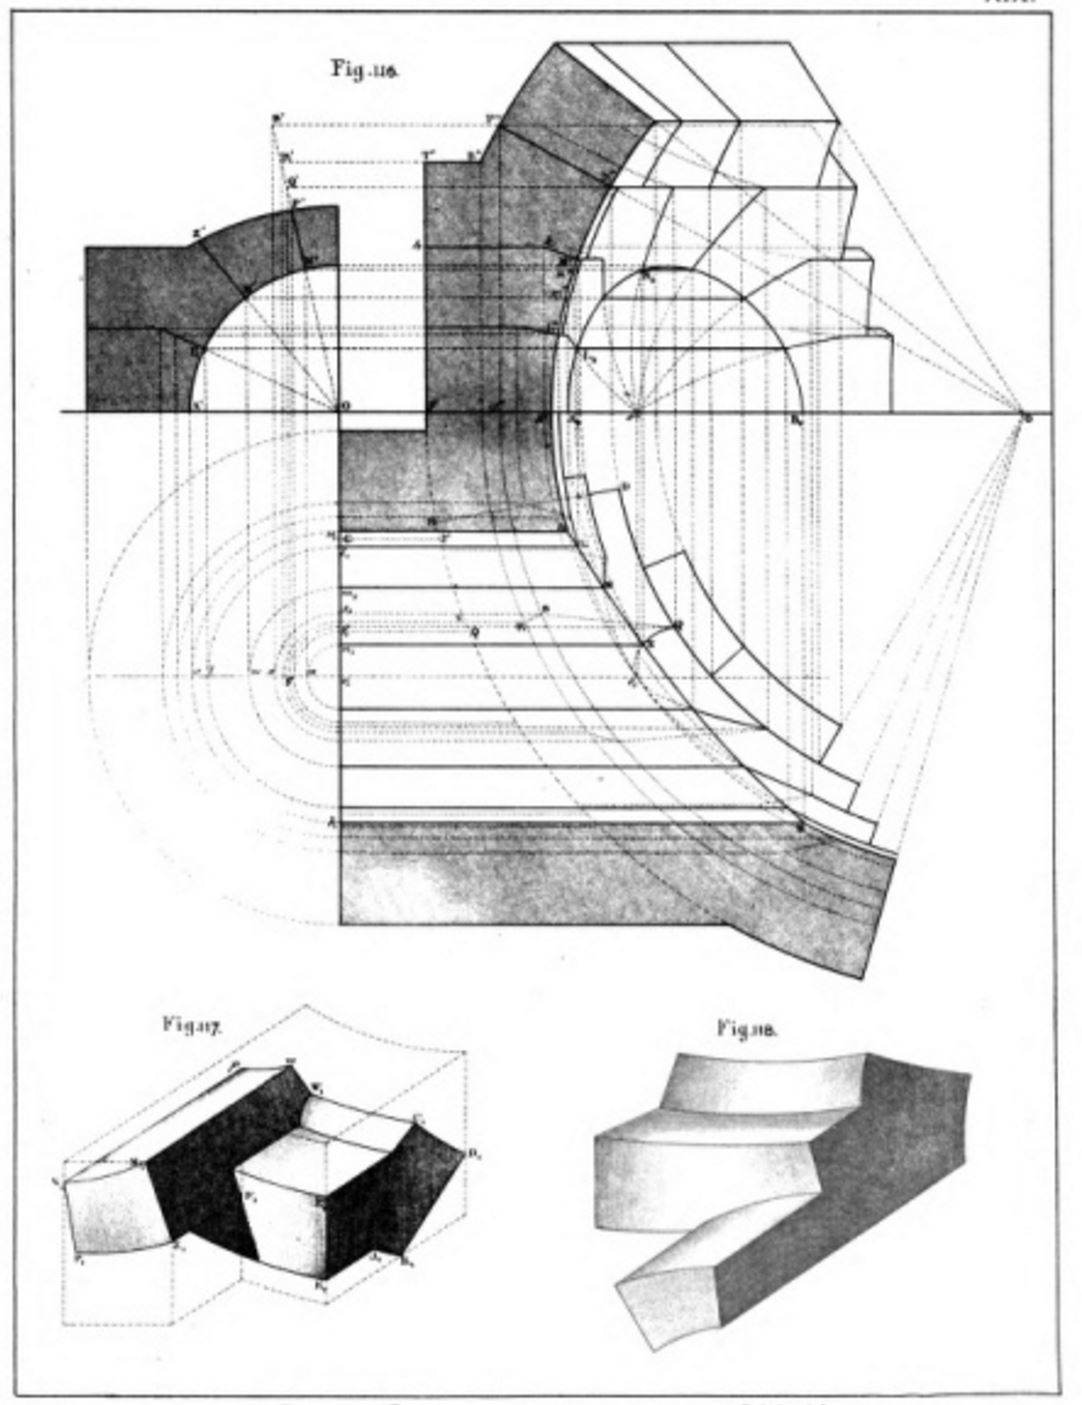
\includegraphics[width=0.45\linewidth ]{figure/Introduction/NotesonStereotomy.JPG}
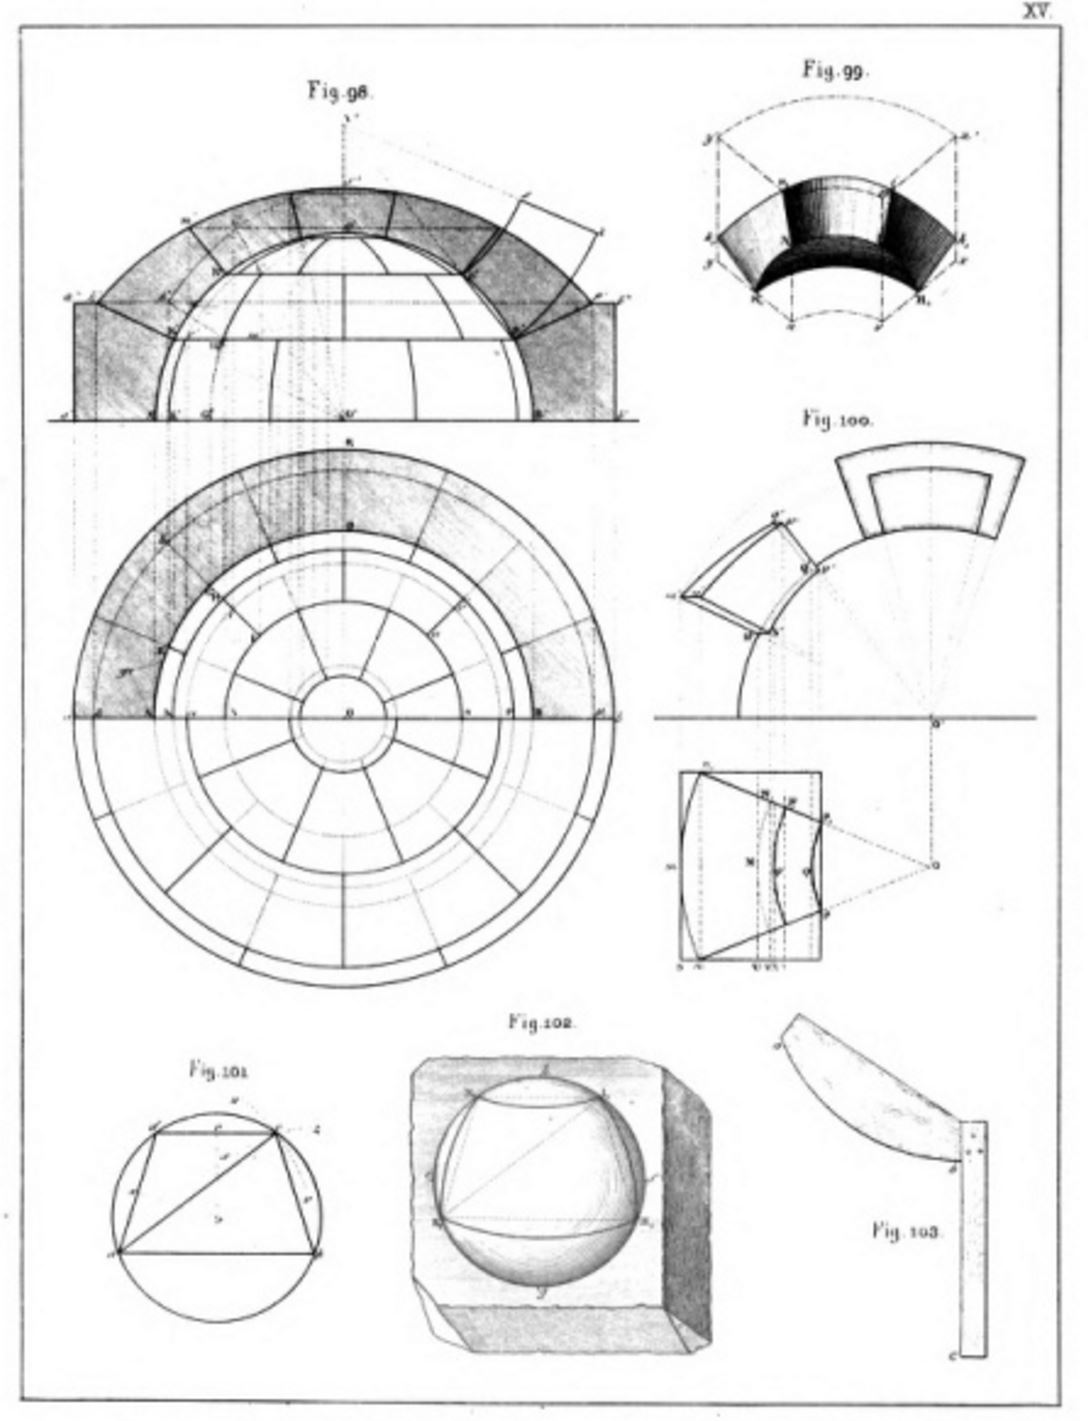
\includegraphics[width=0.45\linewidth ]{figure/Introduction/NotesonStereotomy2.JPG}
\caption{The length of the curve is the same regardless of coordinate system.}
\end{figure}

It was used early as an tool for subdividing shapes into building elements that would be able to cut and fit together. Wellknown in this field is Philibert de l'Orme from France that was active during the 16 th century. Long before computers he managed to create astonishing structures and patterns of very complex surfaces.

\begin{figure}[H]
\centering
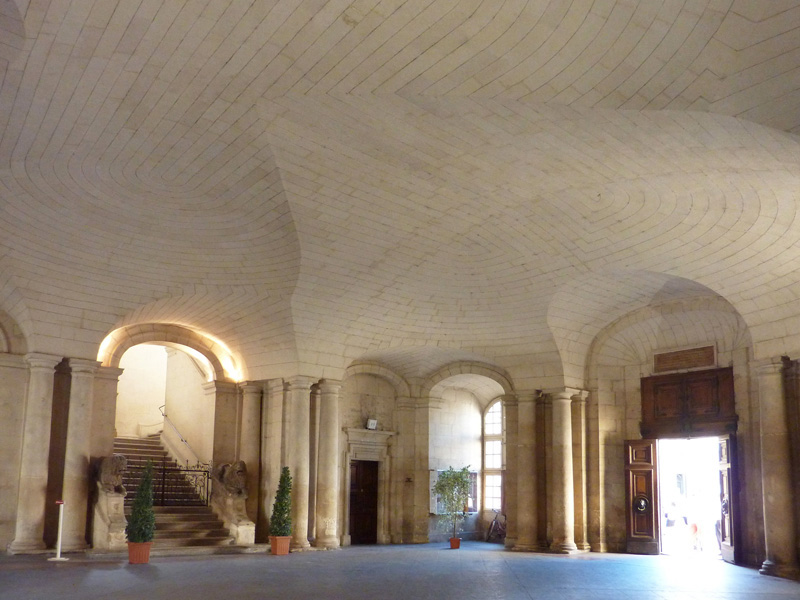
\includegraphics[width=0.90\linewidth ]{figure/Introduction/Arles.jpg}
\caption{The length of the curve is the same regardless of coordinate system.}
\end{figure}

This techniques are not very common today since it involves quite complex building elements that need to be manufactured. Though it is possible to read the research of the Block research group where they have investigated in how to use computational methods and digital fabrication to achieve this structures.


\begin{figure}[H]
\centering
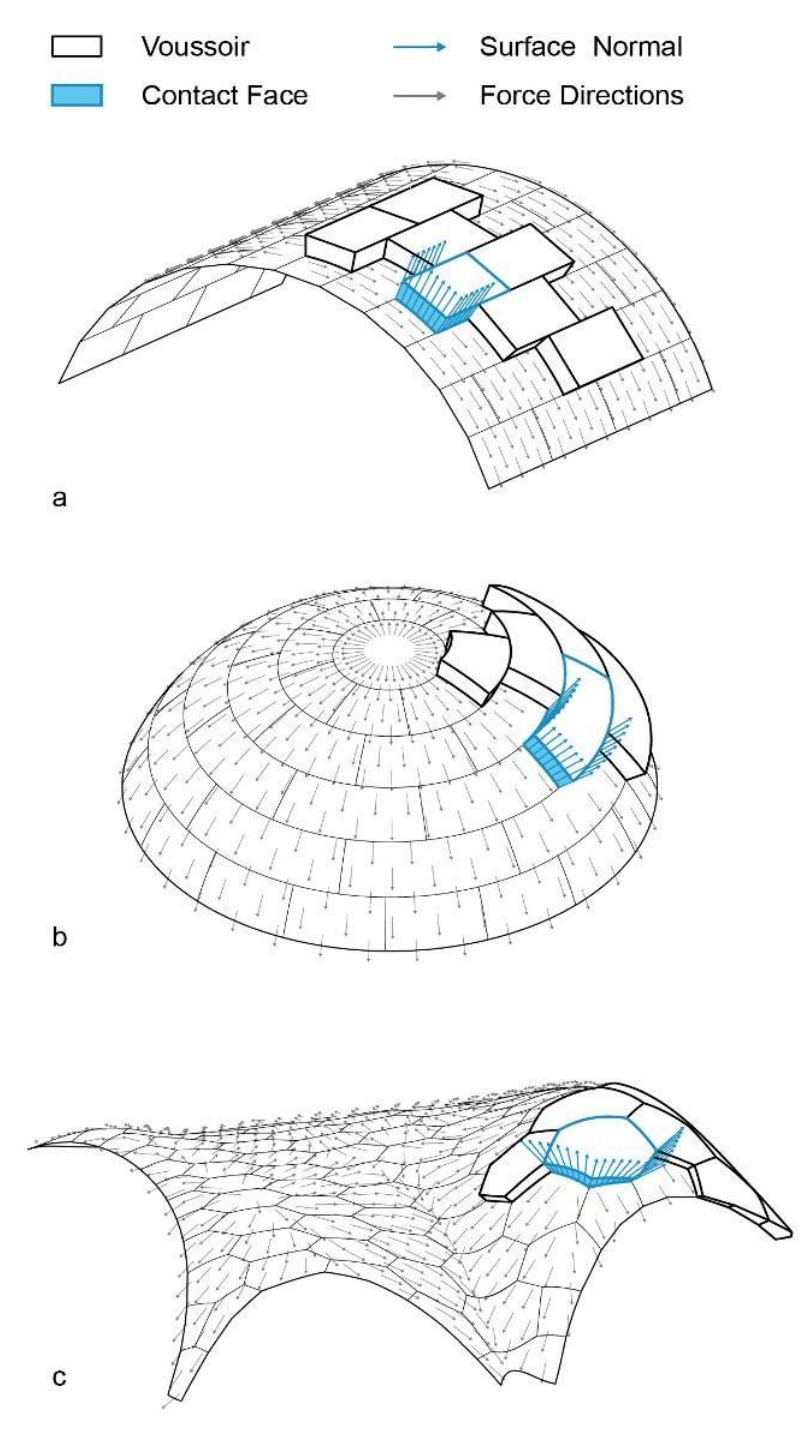
\includegraphics[height=0.50\linewidth ]{figure/Introduction/StereoBlock2.JPG}
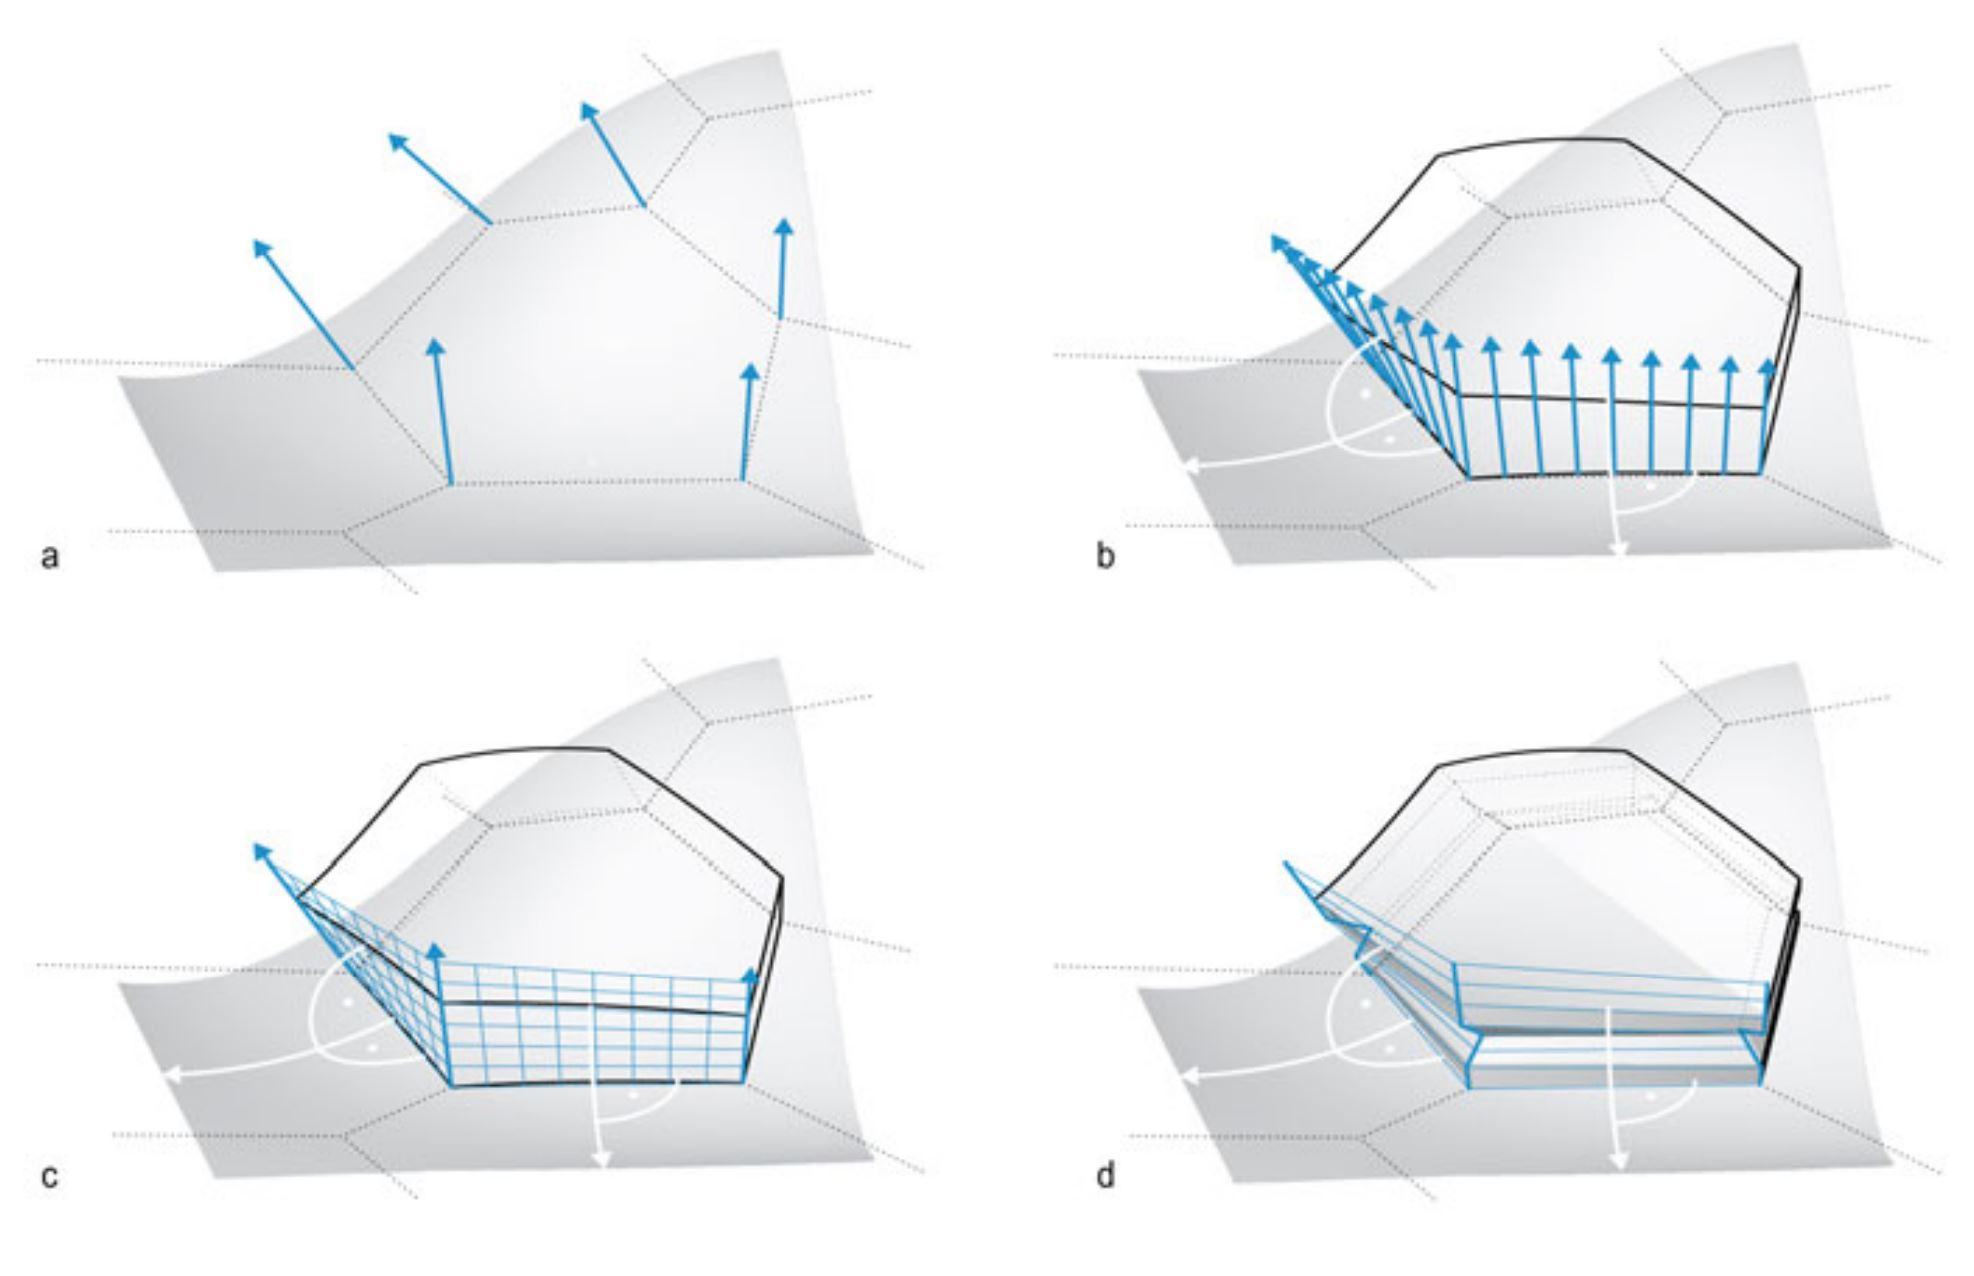
\includegraphics[height=0.35\linewidth ]{figure/Introduction/StereoBlock.JPG}
\caption{The length of the curve is the same regardless of coordinate system.}
\end{figure}



\begin{figure}[H]
\centering
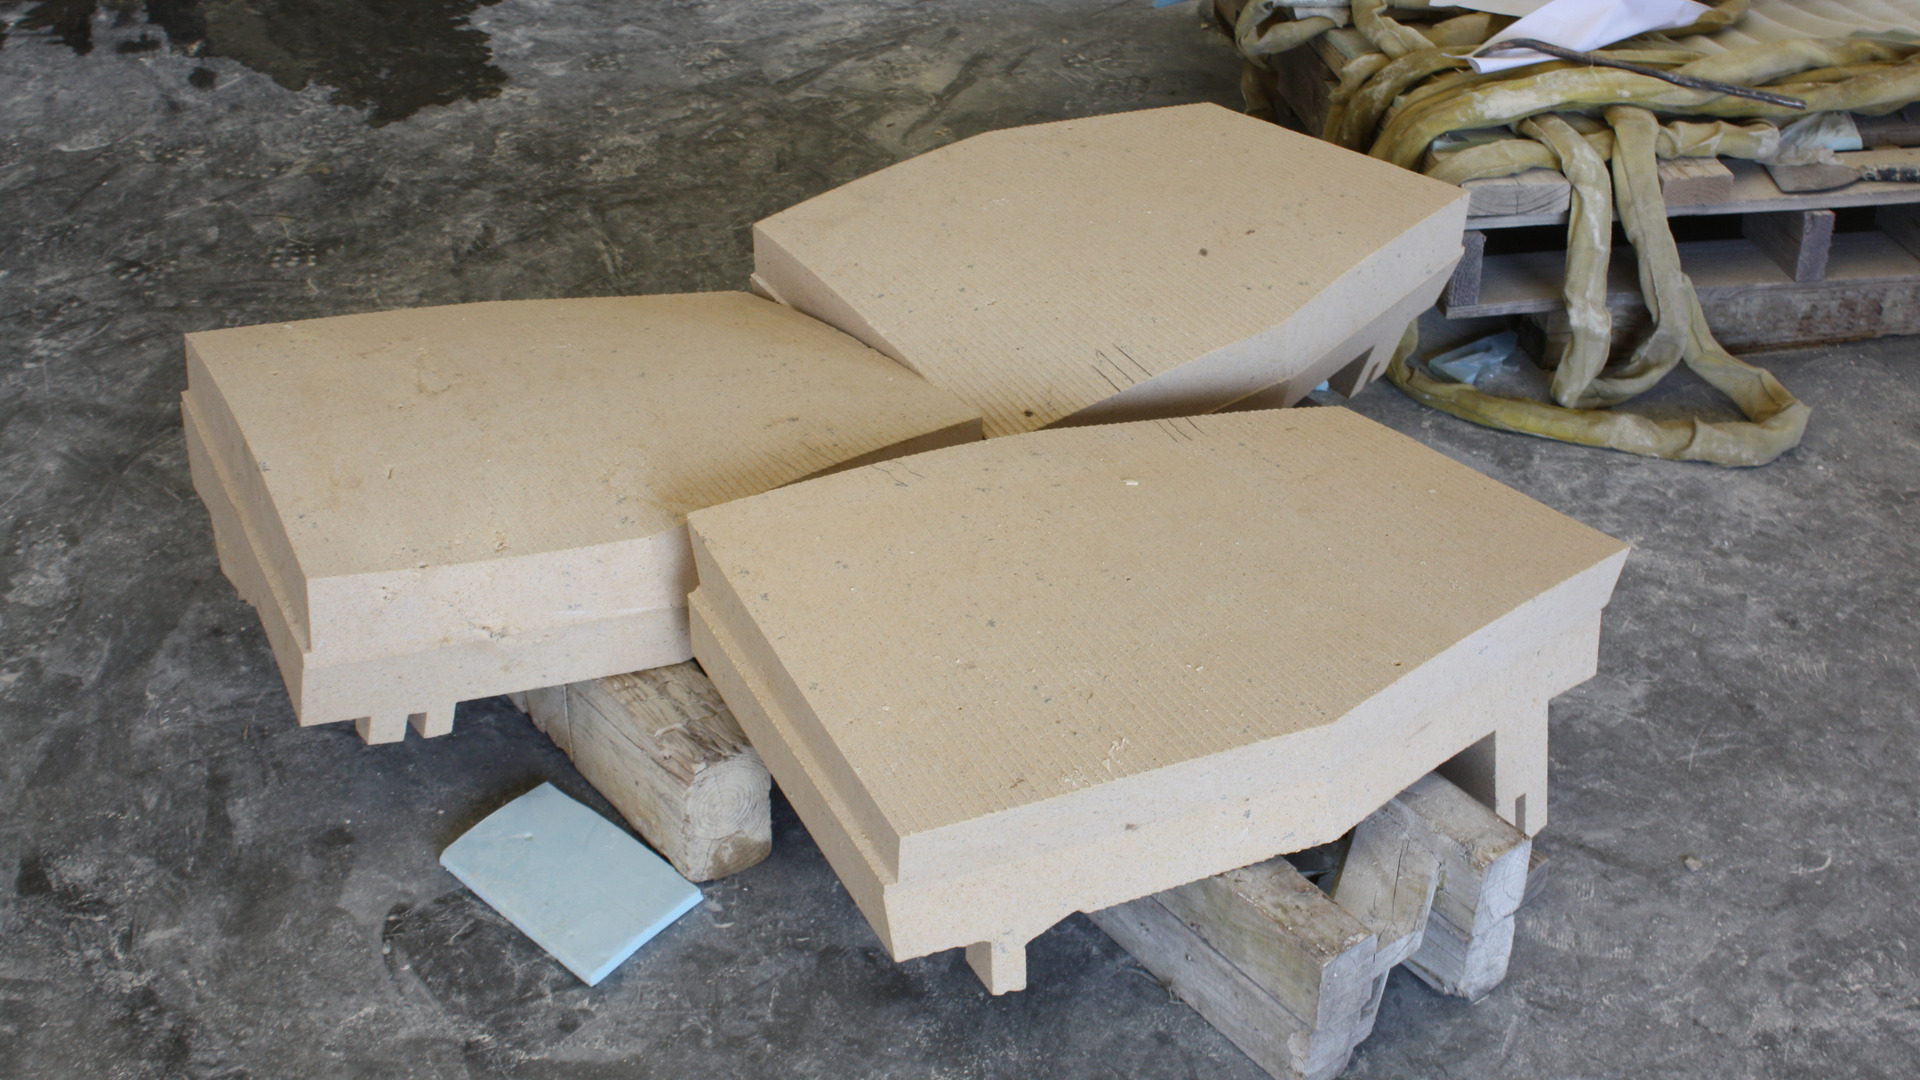
\includegraphics[height=0.4\linewidth ]{figure/Introduction/blockStereo.jpg}
\caption{The length of the curve is the same regardless of coordinate system.}
\end{figure}


\subsection{Geometry in Architecture}

It is really hard to think of architecture without the tools of geometry and math since it makes it presence in most things we do. It is such a crucial part in communicating and describing projects in drawings and models. Looking at historical examples architecture has been highly influenced
by proportions and patterns. It has also been a necessary tool until this day for the realisation of buildings and its elements. Comparing the engineer and architect of today with one of some hundreds of years a ago the geometrical  understanding was probably greater before due to the lack of  all the modern tools and software's that do the math for us today.  



\begin{figure}[H]
\centering
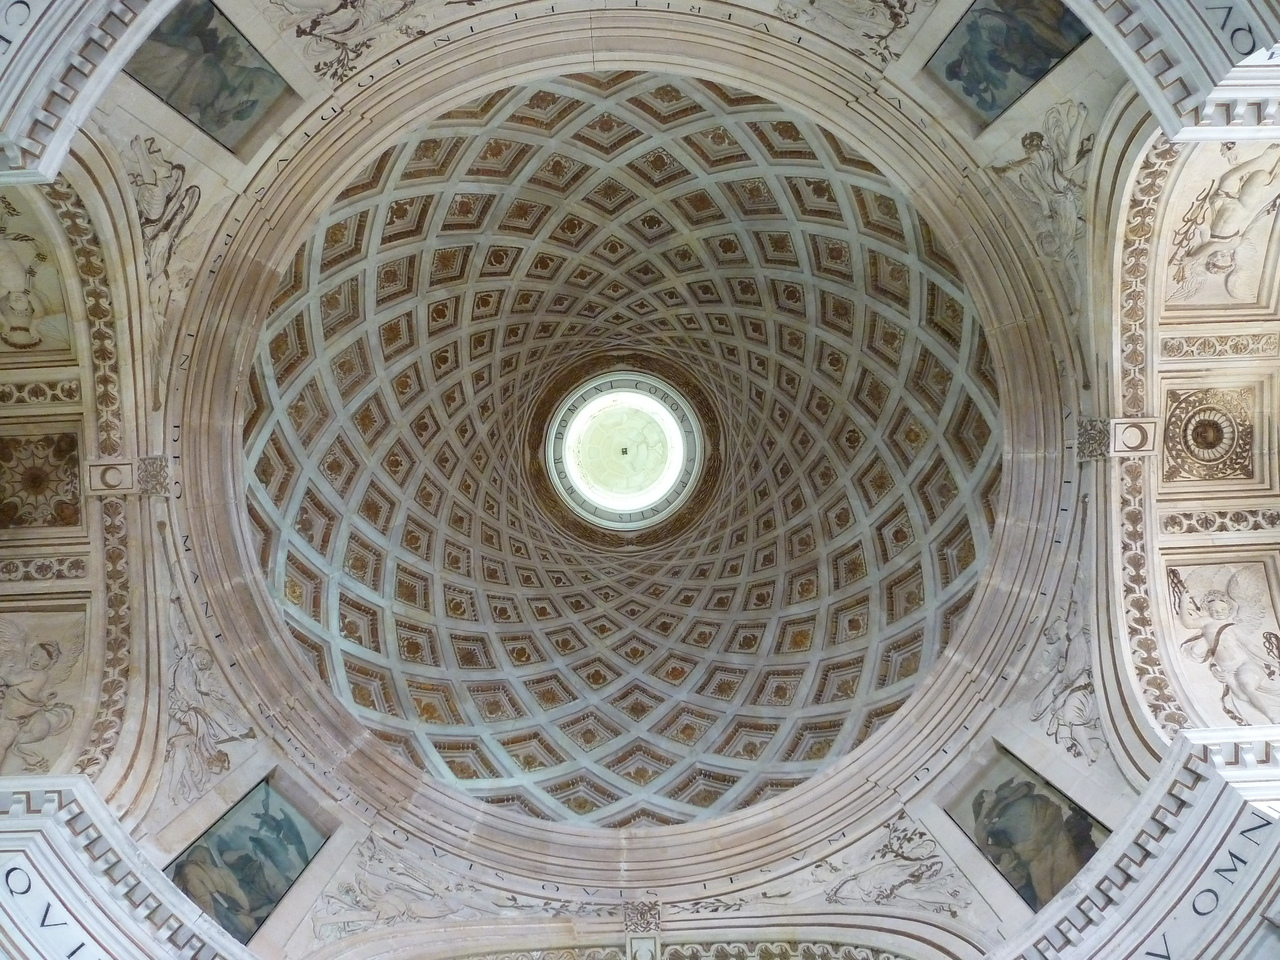
\includegraphics[height=0.45\linewidth ]{figure/Introduction/PhillibertDeLorme.jpg}
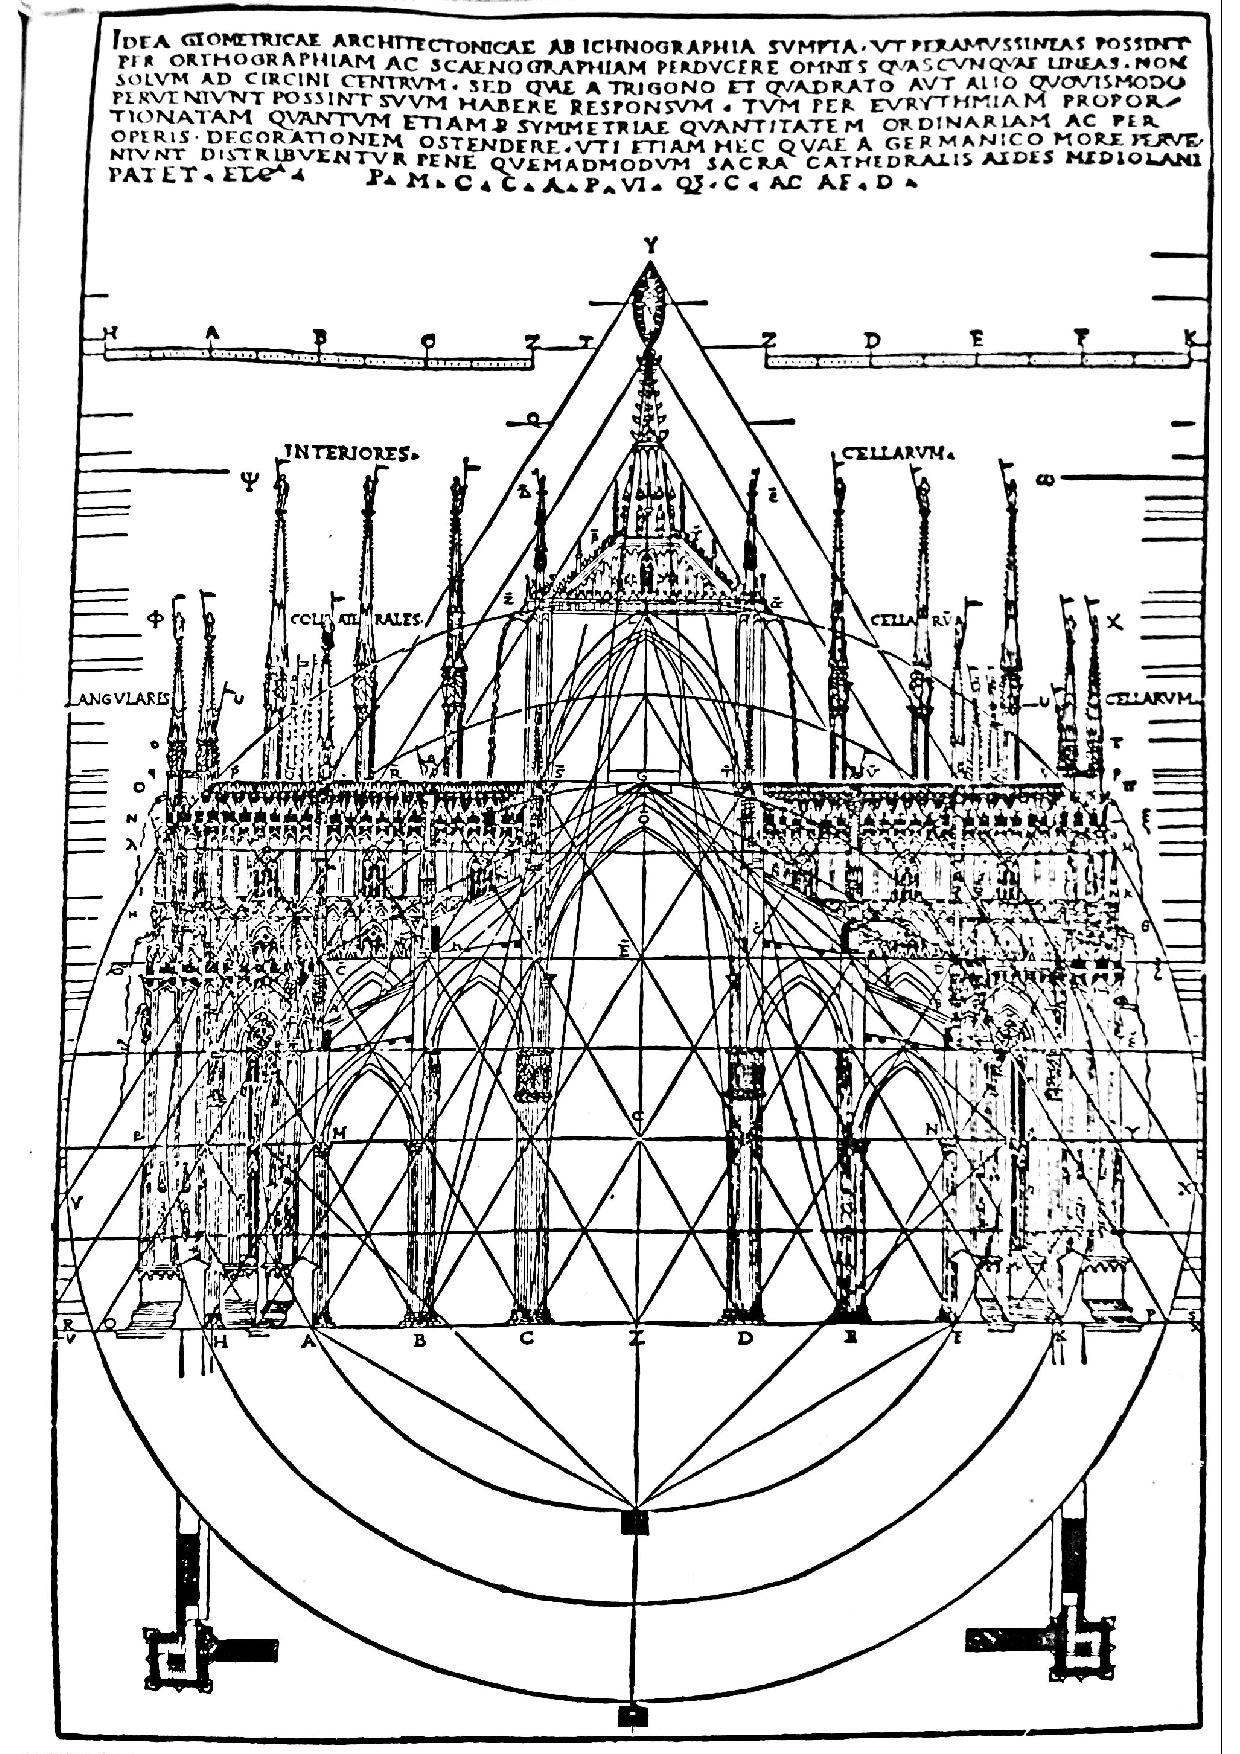
\includegraphics[height=0.45\linewidth ]{figure/Introduction/Milan.pdf}
\caption{The length of the curve is the same regardless of coordinate system.}
\end{figure}

\subsubsection{Application in Modern architecture }
The use of mathematical proportions and symmetries in projects has been out of fashion in the 20th and 21th century architecture. If expressive geometry and symmetry has been associated with harmony in the past it nowadays it is more focused to rational and complex buildings. Rational where you need a cheap and efficient structural system to handle forces or easy assembling or manufacturing. Complex when you have a form you want to achieve when complex mathematics is the only way of achieving realisation. There are certainly engineers and architects that have been able to simple and rational with fascinating structures and spatial experiences. Norman Foster, Pier Luigi Nervi, Buckminster Fuller are a few in this category. Nervi made many structures with big spans such as sports arenas and exhibition halls. Noticeable is that the geometry is often incorporated with the functionality of the structure.


\begin{figure}[H]
\centering
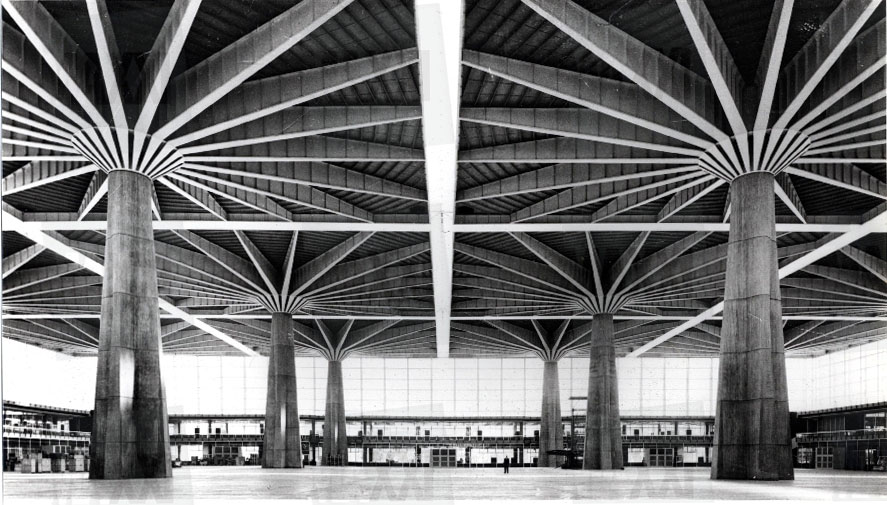
\includegraphics[height=0.4\linewidth ]{figure/Introduction/Nervi3.jpg}
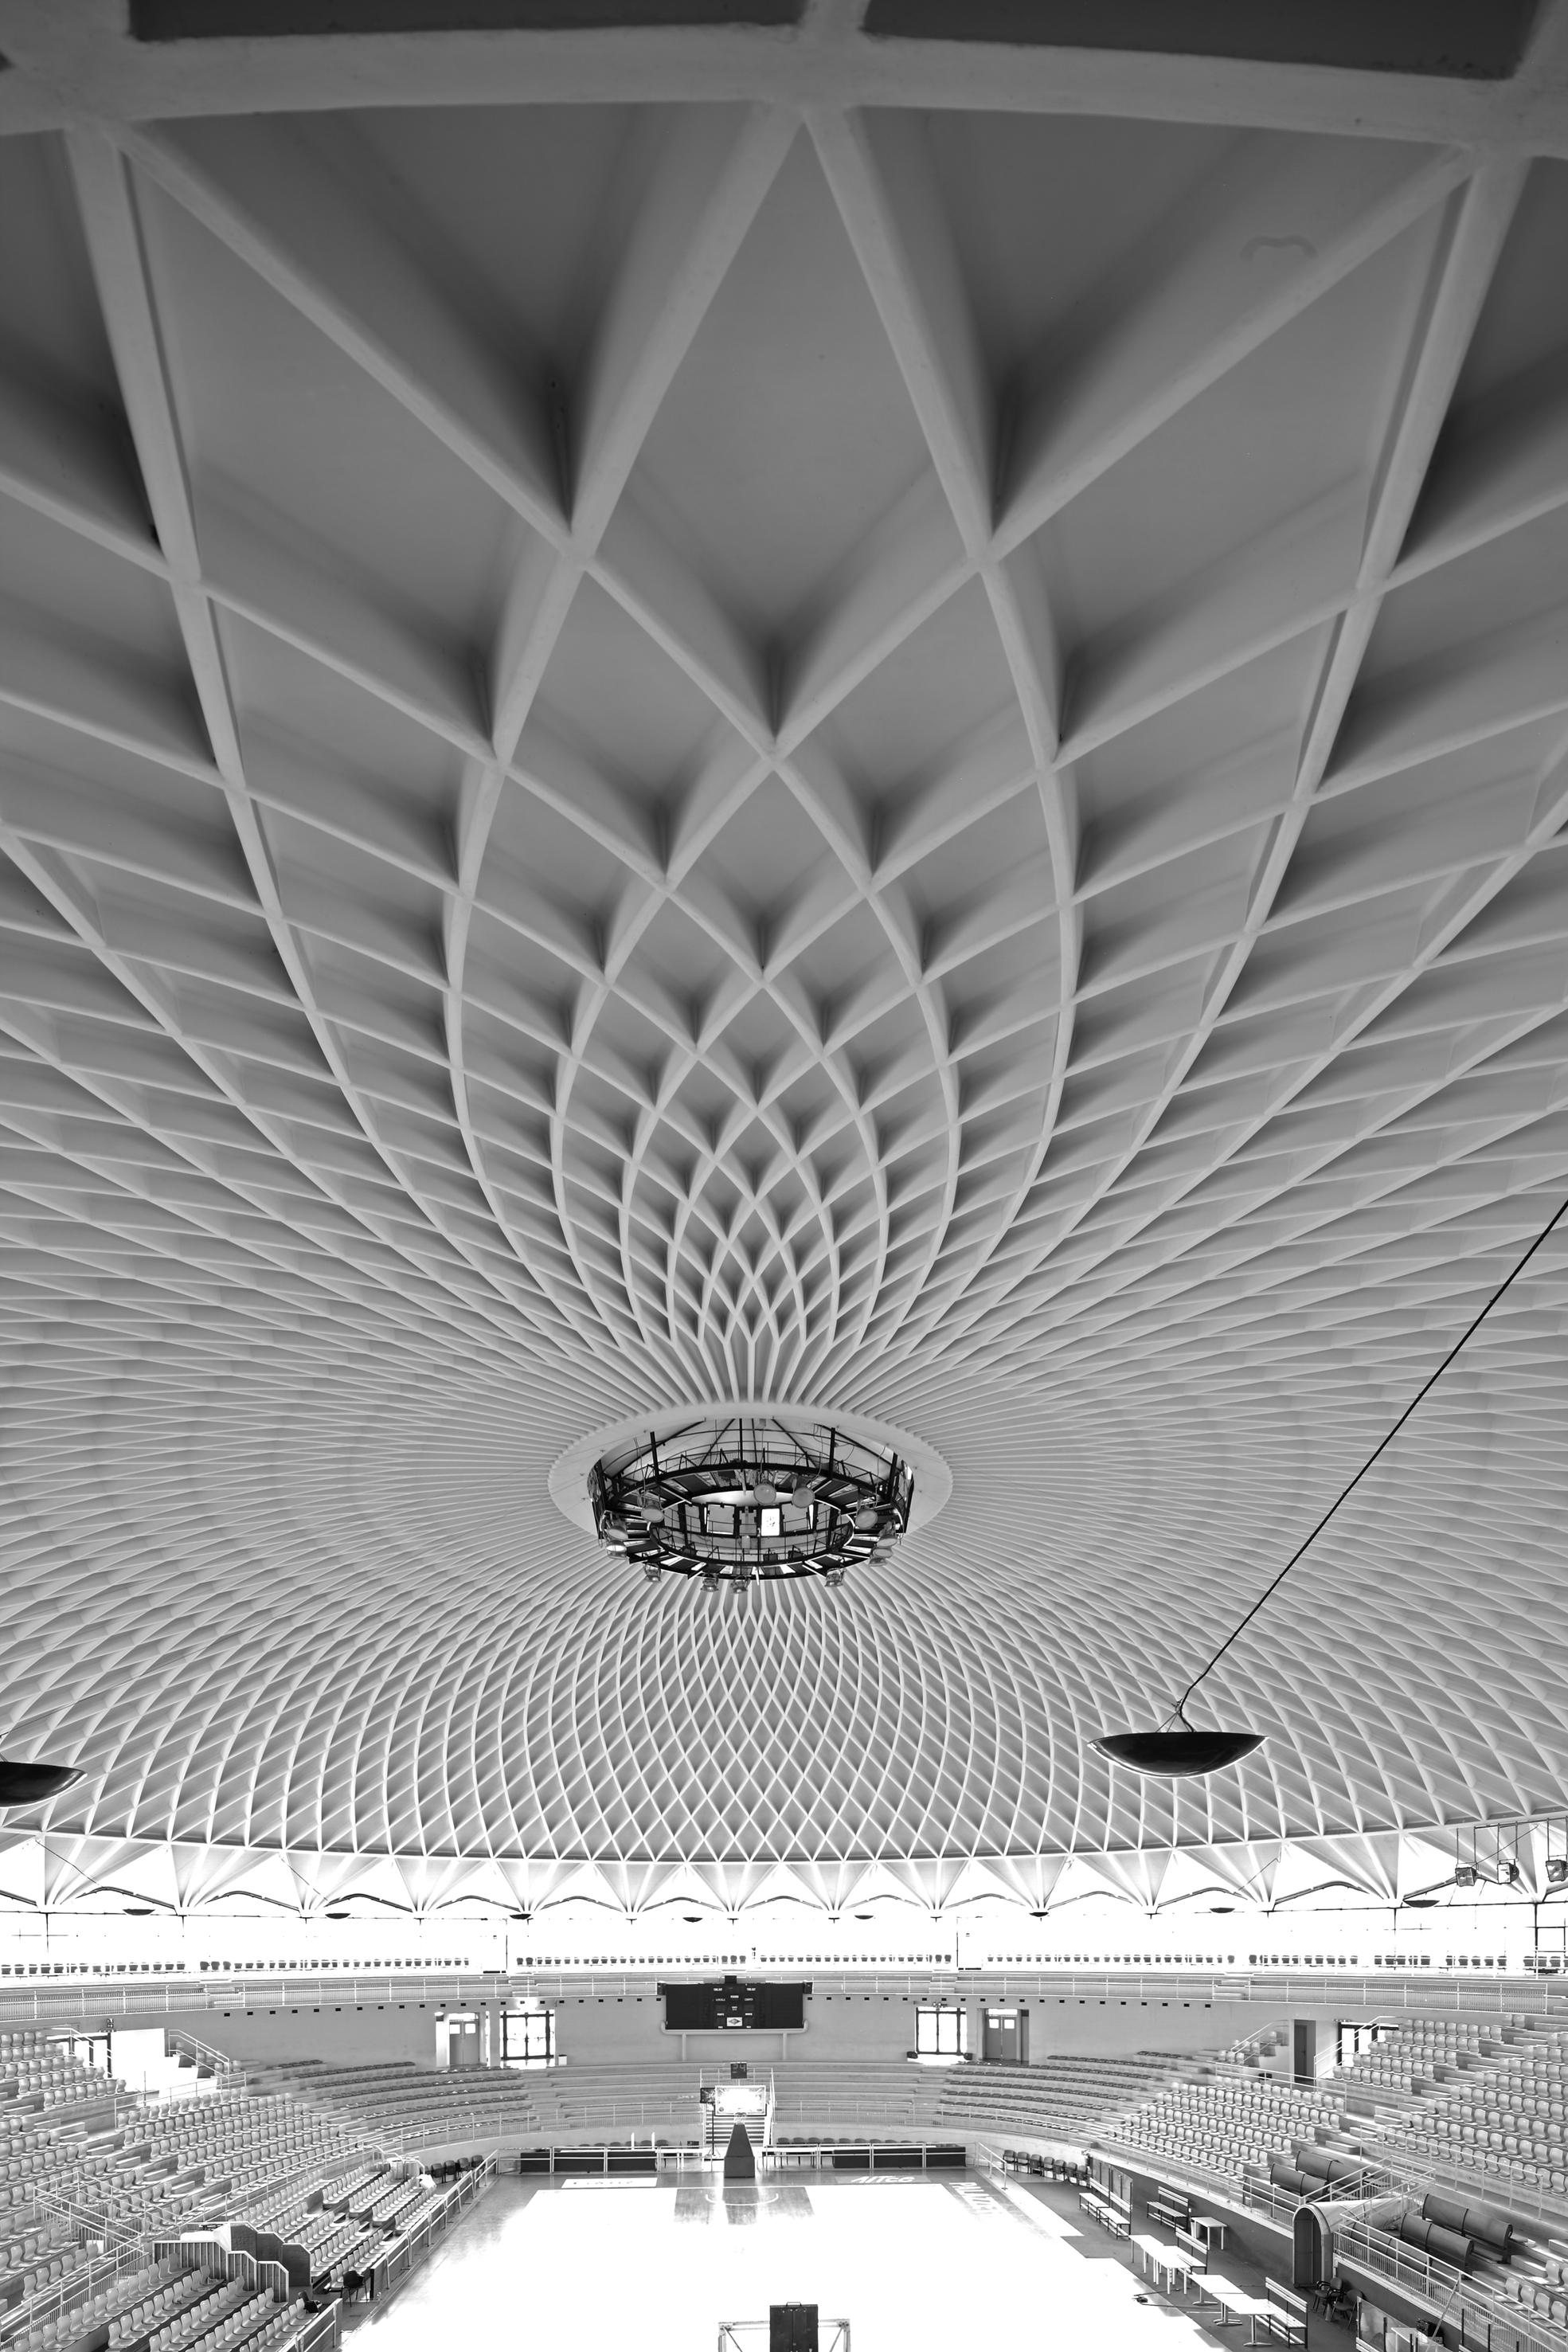
\includegraphics[height=0.4\linewidth ]{figure/Introduction/nervi4.jpg}
\caption{The length of the curve is the same regardless of coordinate system.}
\end{figure}


Both Fuller and Foster has expressed deep commitment in how their design can shape the society. Fuller is often associated with the geodesic dome and tensigrity structures. This is of course true but it not much in a architectural or sociable aspects in how we live.


\begin{figure}[H]
\centering
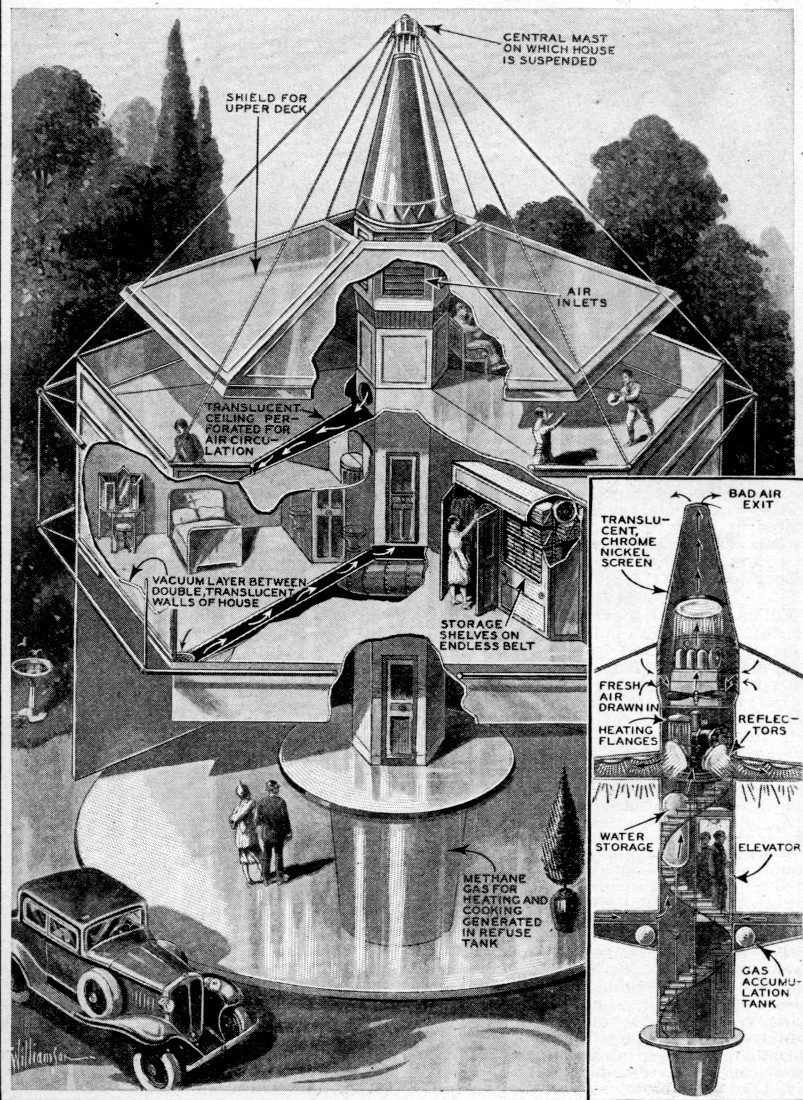
\includegraphics[height=0.45\linewidth ]{figure/Introduction/Fuller2.jpg}
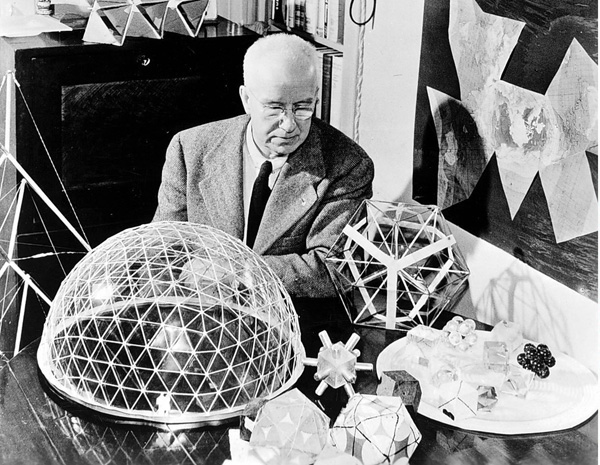
\includegraphics[height=0.45\linewidth ]{figure/Introduction/fuller3.jpg}
\caption{The length of the curve is the same regardless of coordinate system.}
\end{figure}






  

\subsection{Brick Structures}

What is typical for a brick structure is uniformity of its building elements, the brick. The brick is made of clay can be formed into nearly any shape, but the most common is the cuboid. The way the brick is made affects its colour, shape, texture, strength, Resistance to fire and weather and longevity. This means that strangely enough both the diversity and the unity are the most striking features of the structure. Looking at a traditional building the brick composition becomes a patchwork of different colours, the shape has small deviations due to imperfections of the shape and the roughness of the texture. Even though we have modern techniques and methods to make the colours, shape and texture uniform it is mostly common to keep or resemble these imperfections.\\
Two other important aspects of a brick structure is the mortar and the skills and creativity of the craftsman. The mortars main purpose is to bond the bricks together into a structure and to compensate the differences of the bricks. 

\begin{figure}[H]
\centering
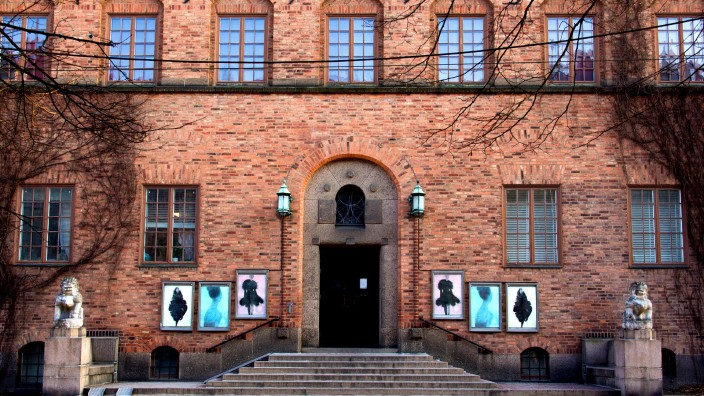
\includegraphics[width=1.0\linewidth ]{figure/Introduction/Rohsska.jpg}
\caption{Rhösska museum in Gothenburg.}
\end{figure}







\subsubsection{Types of Bricks}

There are two basic types of brick: fired bricks and sun bricks. The former is made heating it in a kiln and the other is dried in the sun. The most common used in modern world is the fired brick. 

\subsubsection{Brick Making}

\begin{figure}[H]
\centering
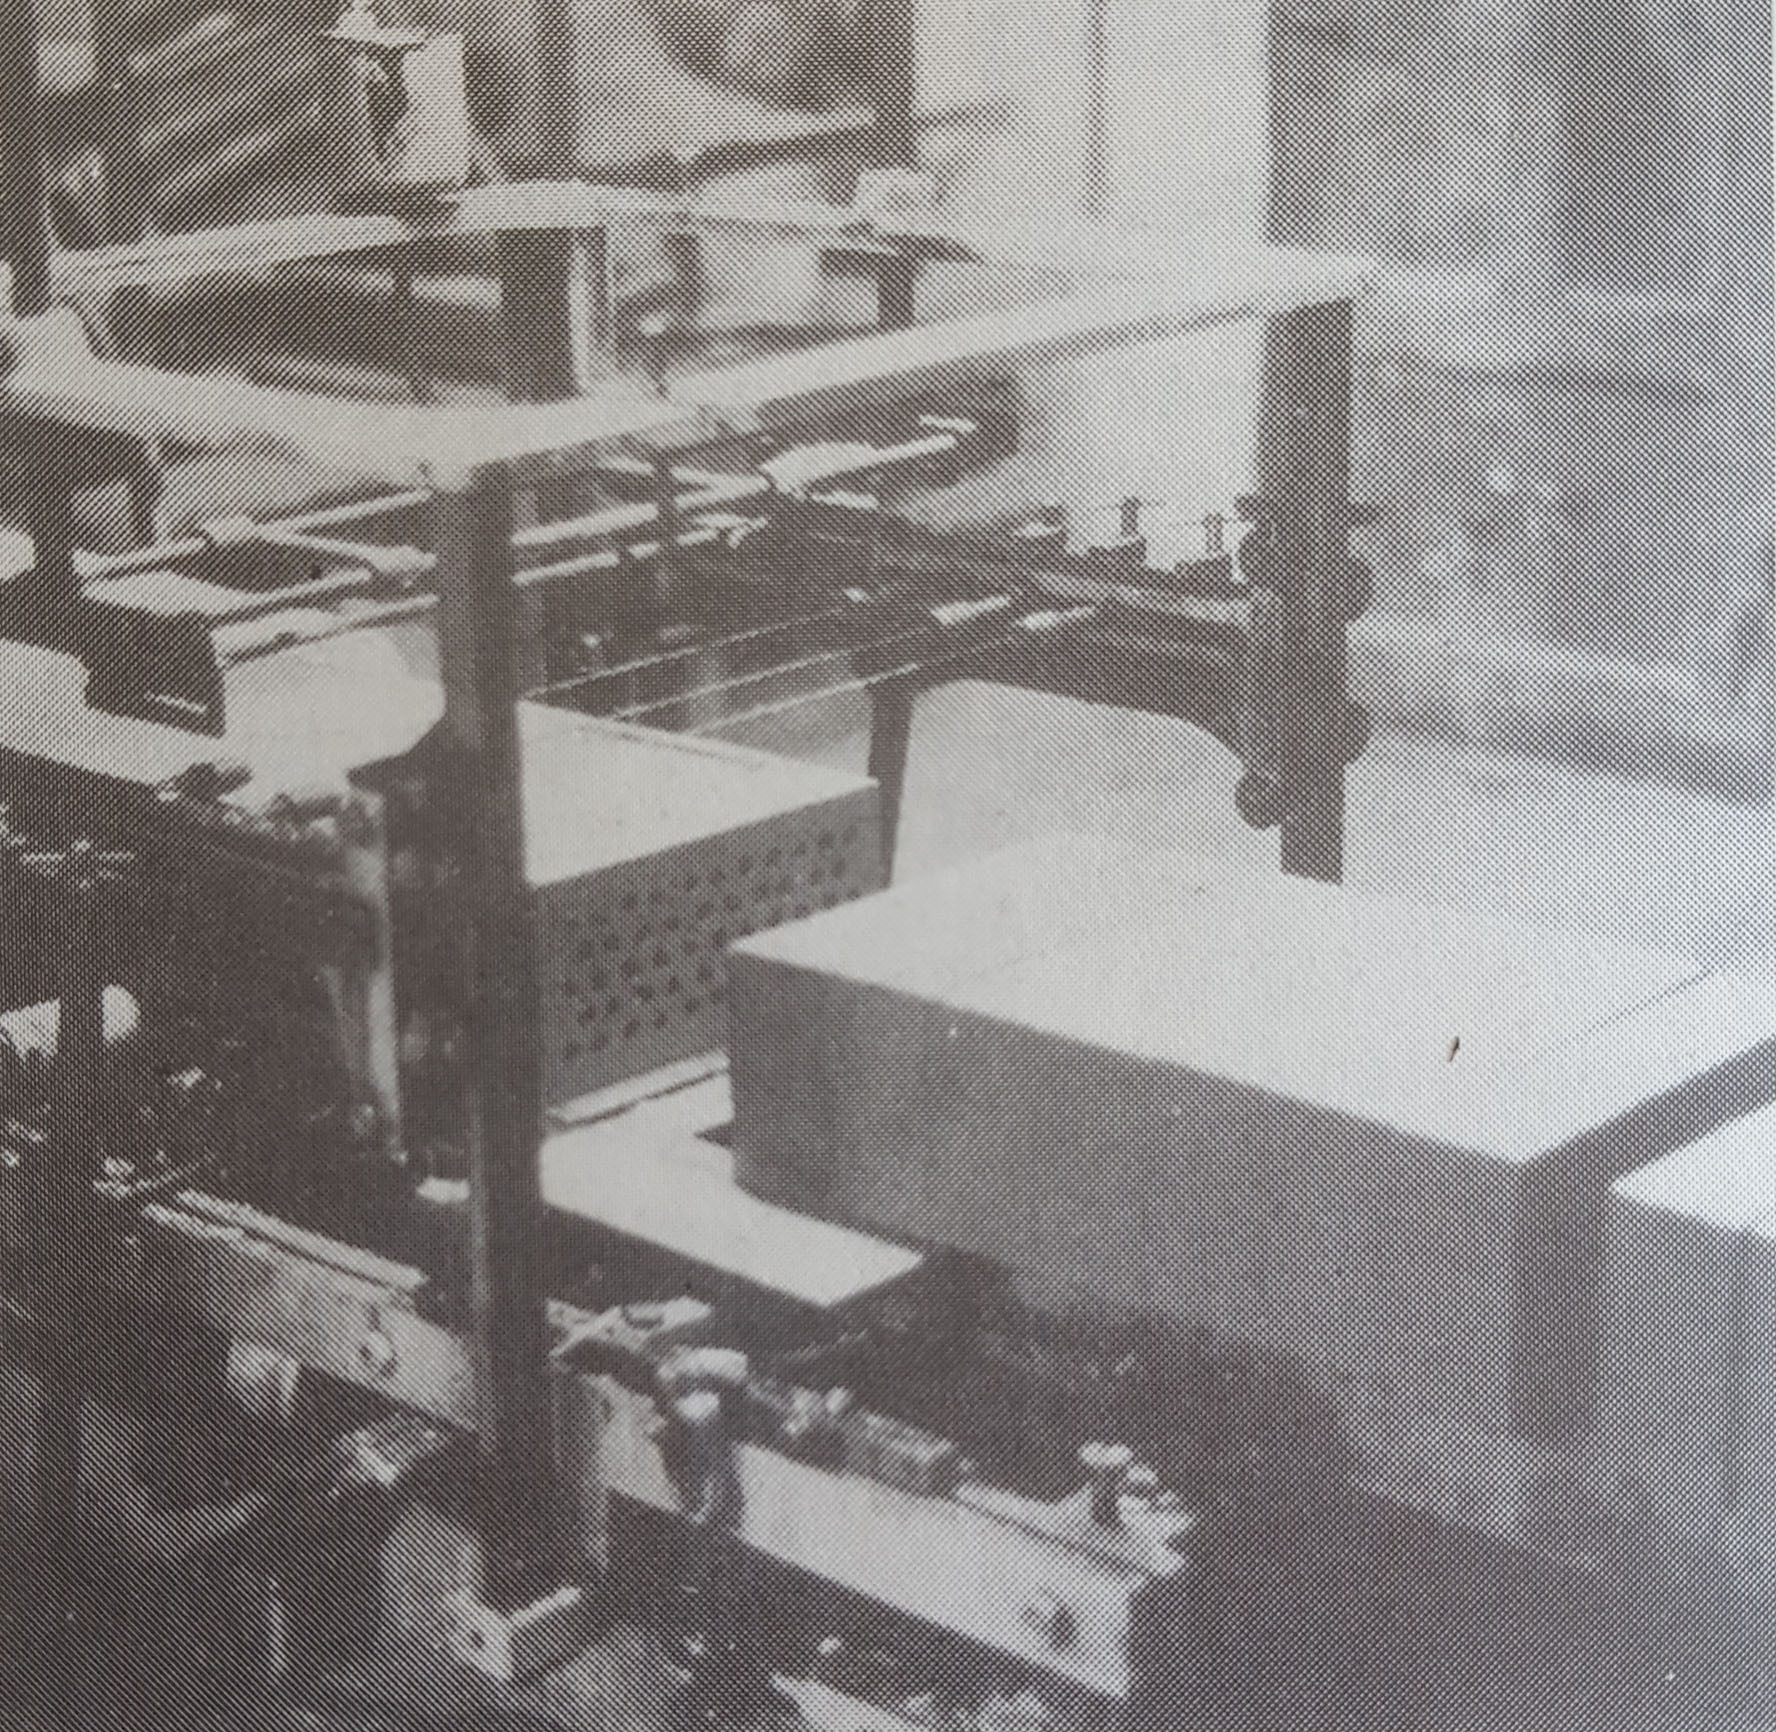
\includegraphics[width=0.9\linewidth ]{figure/Theory/wireBrick.jpg}
\caption{The length of the curve is the same regardless of coordinate system.}
\end{figure}

\begin{figure}[H]
\centering
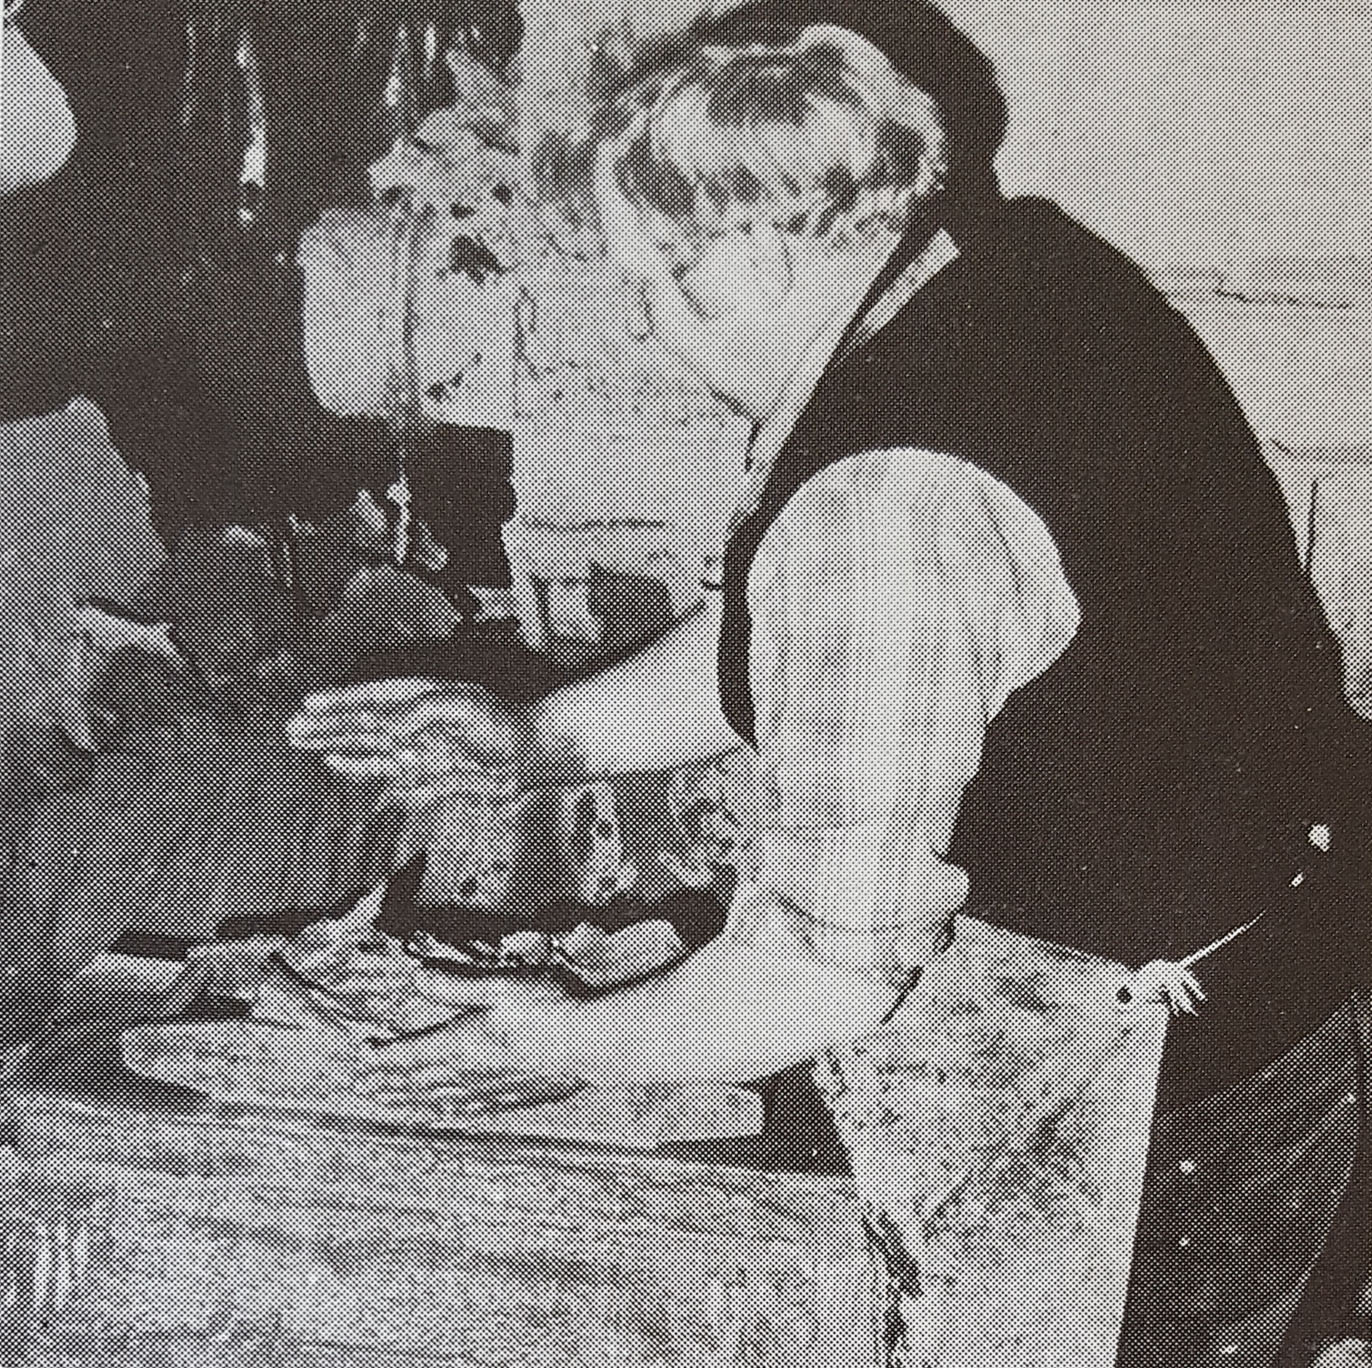
\includegraphics[width=0.3\linewidth ]{figure/Theory/brickmaking2a.jpg}
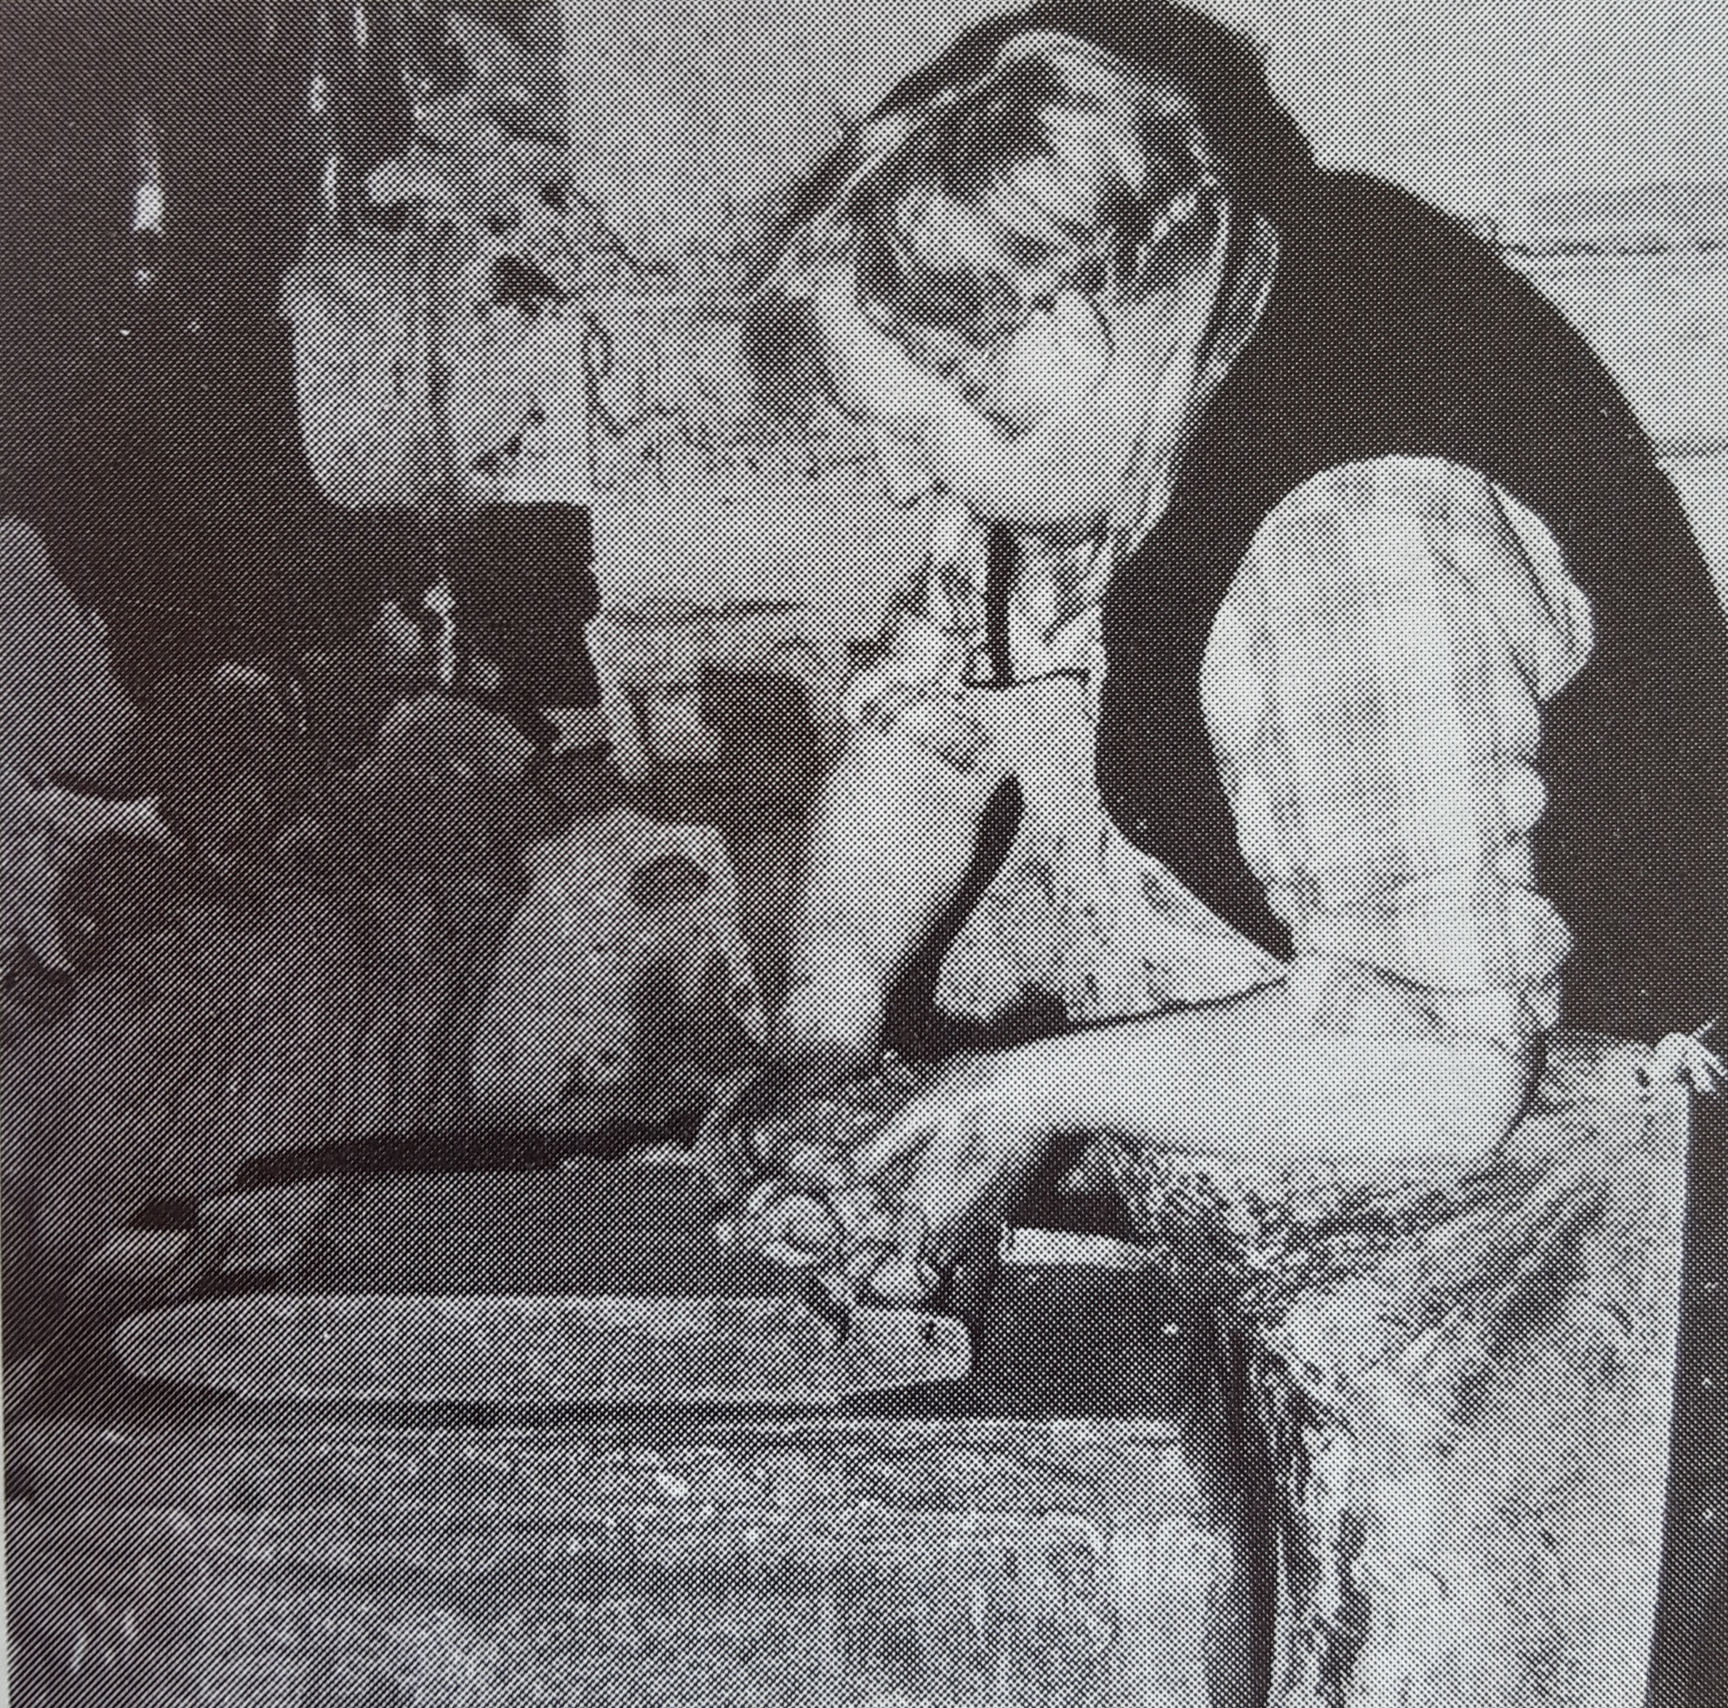
\includegraphics[width=0.3\linewidth ]{figure/Theory/brickmaking1.jpg}
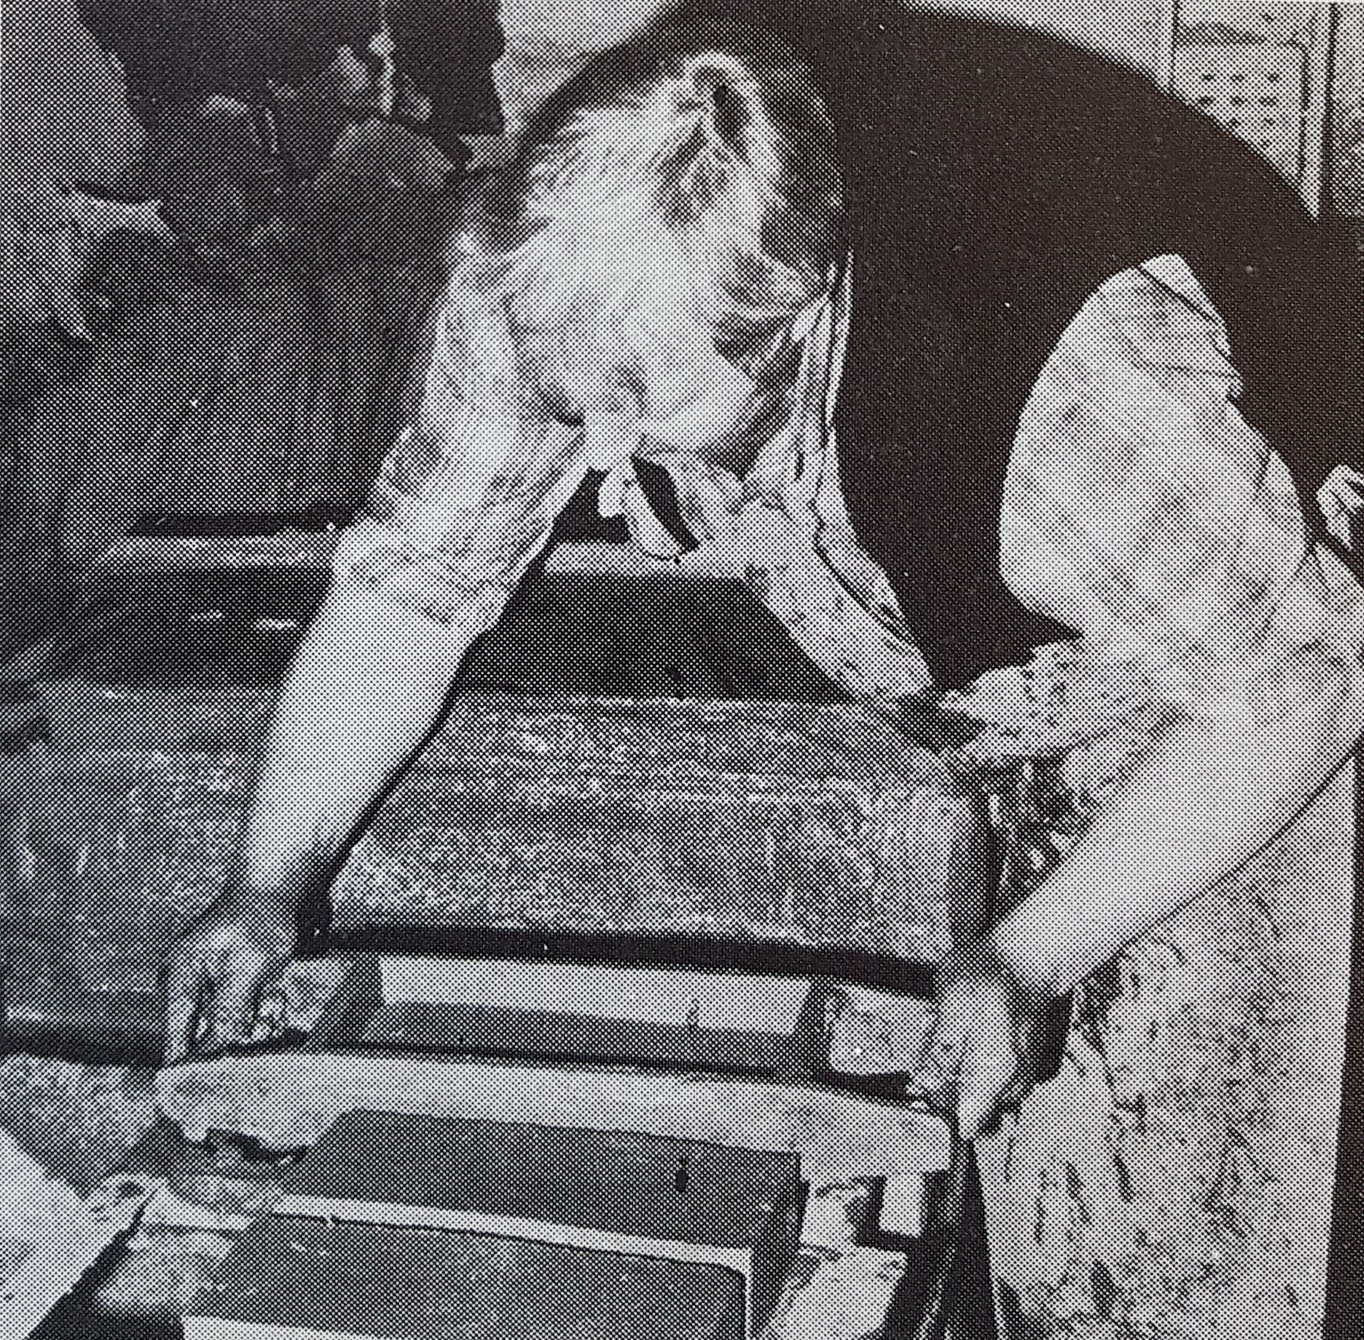
\includegraphics[width=0.3\linewidth ]{figure/Theory/brickmaking2b.jpg}
\caption{The length of the curve is the same regardless of coordinate system.}
\end{figure}

\subsubsection{Mortar}

Mortar is  material used in building construction to bond brick, stone, tile, or concrete blocks into a structure. Mortar consists of inert siliceous (sandy) material mixed with cement and water in such proportions that the resulting substance will be sufficiently plastic to enable ready application with the mason’s trowel and to flow slightly but not collapse under the weight of the masonry units. Britannia \\

Main ingredients of mortar are:
\begin{itemize}
\item \textit{Water}
\item \textit{Aggregates}
\item \textit{Binder}
\item \textit{Admixtures}, examples of are: plasticisers,super plasticisers,accelerators, retarders, air entraining agents. 
\item \textit{Pigments}


\end{itemize}

\paragraph{Aggregates}~\\
The aggregates in mortar is mostly \textit{sand}. Sand is a rock mixture of rock particles of different sizes from 10 mm in diameter down to 75$\mu$m. 


\paragraph{Binders}~\\  Widely used binders are based on one of these categories
\begin{itemize}
\item \textit{Hydraulic cements}, which reat chemically with water at normal site temperatures.
\item \textit{lime-silica mixtures}, which react only in the presence of high-pressure steam.
\item \textit{lime-pozzolan mixtures}, which set slowly at ambient temperatures, or pure lime which sets slowly in air by carbonation.  
\end{itemize}
\paragraph{Admixtures}


\begin{itemize}
\item Pozzolanic mortar
\item Lime mortar
\item Portland Cement mortar
\end{itemize}

\subsubsection{Material Properties}
There are some general properties that applies to clay based ceramic materials.\\

\begin{itemize}
\item Hard and brittle
\item Momentanelastiska(engelska??),
i.e. they have almost no creep and plastic deformation
\item Thermal resistant(värme beständinga)
\item Resistant against acid and biological attacks
\item Have small volumetric deformations,
i.e. no deformations related to heat and moisture.
\item High electrical resistivity  (elektriskt isolerande)
\end{itemize}

The exact properties are much related to the composition of the raw material and the kiln temperature. Even though the brick is the main component of the brick wall you must take into consideration the mortar to get the properties of the brick wall composition.

\subsubsection{Craftsmanship}

It is usually quite hard to get good records on exactly how the role of the bricklayer has been through time. Looking at the tools of today it is quite hard to believe that there has been any dramatic development in this area for hundred or thousands of years. The tools of the bricklayer are quite conservative looking even at other crafts such as carpenters. Wood workers can for instance have a wide range of electrical tools from screwdrivers to many different saws. The bricklayers tool-set is still occupied by trowels, wooden boards, hammers and spirit levels. Below is picture from a book displaying a typical set of tools for bricklayer.

\begin{figure}[H]
\centering
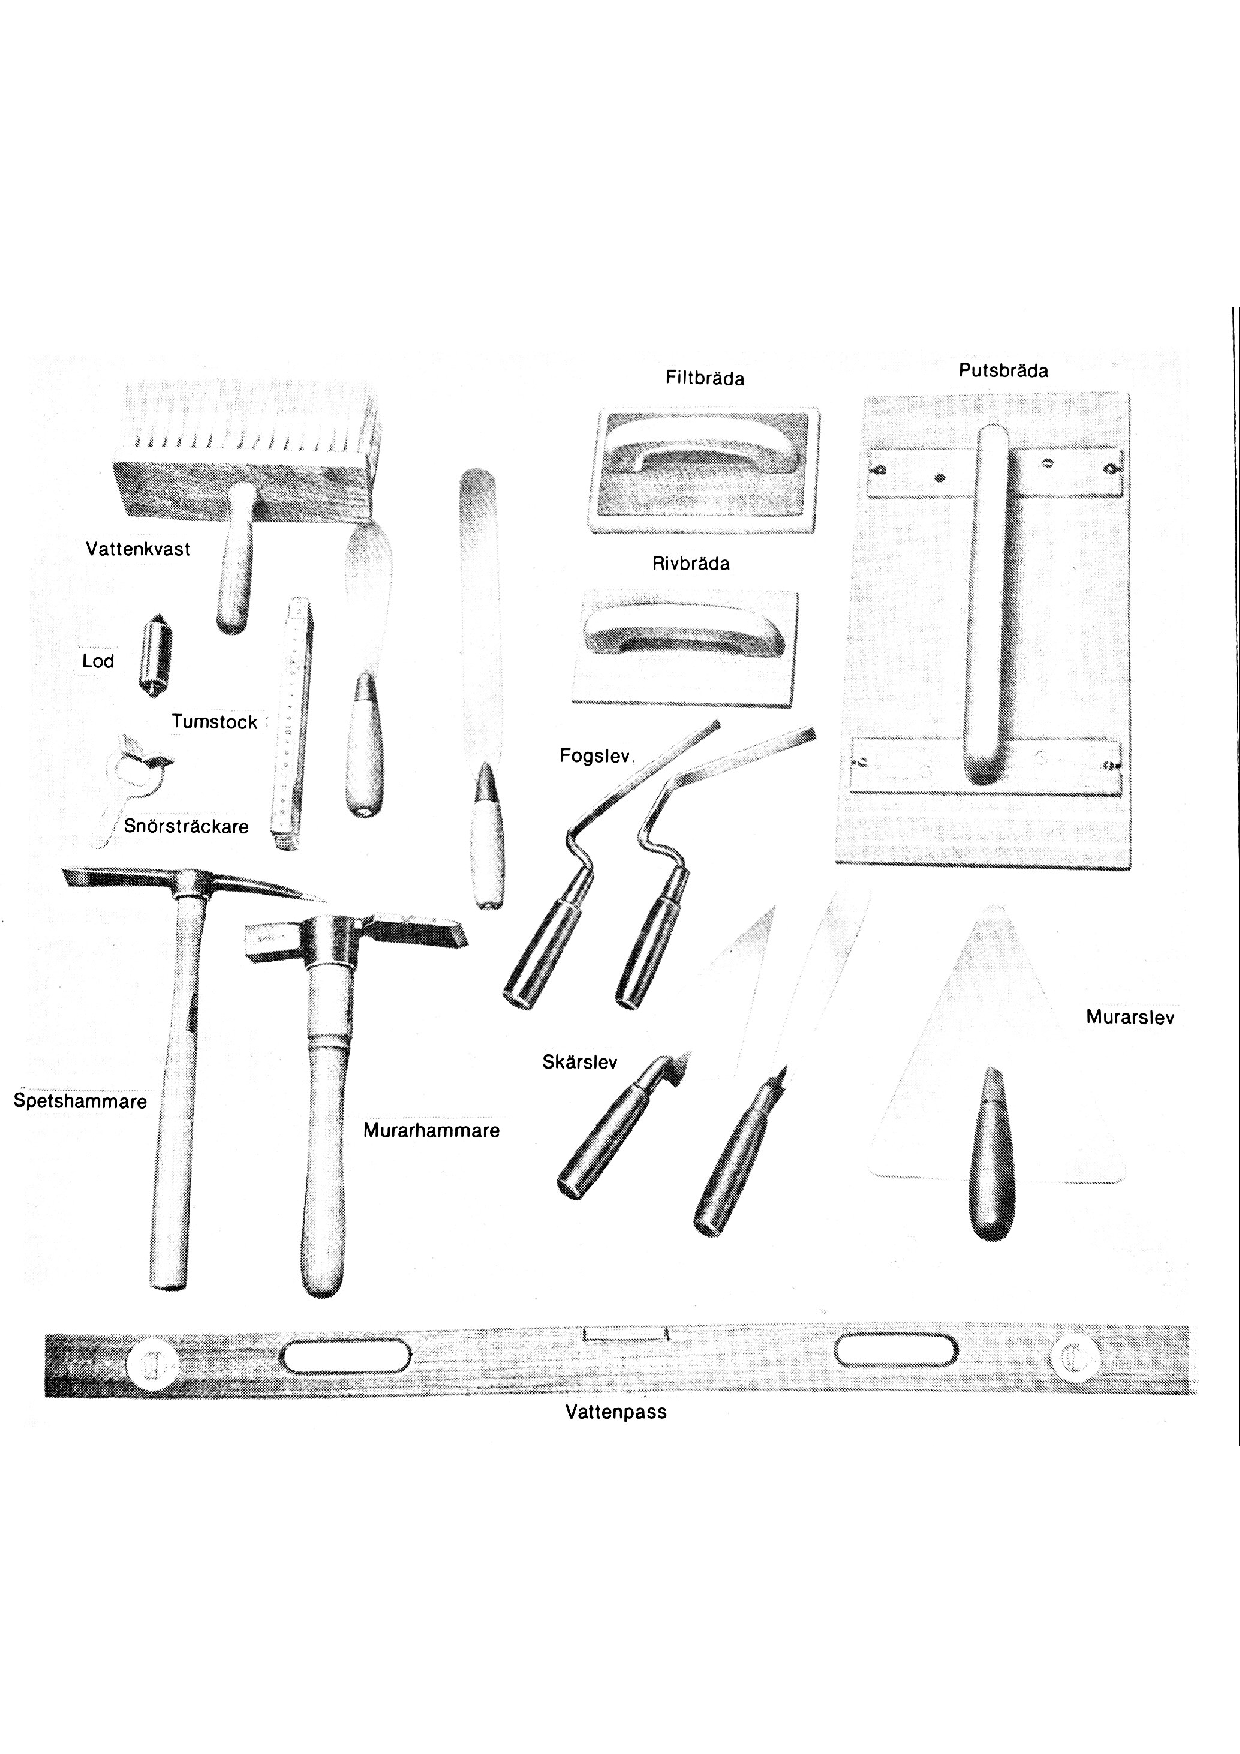
\includegraphics[width=0.8\linewidth ]{figure/Theory/tools.pdf}
\caption{Typical tools for a brick layer}
\end{figure}

The art of bricklaying is to combine  bricks with mortar, which is a workable paste in its initial state that binds the bricks together, to form a composition of structural elements. This composition must meet the requirements of the engineer or architect in terms or geometrical, aesthetic, structural and thermal requirements (it should be dense so that water and air cannot directly pass through). It is a very unforgiving craft since you have no margins for error due to the quick setting of the mortar. If the craftsmanship has been lacking it is very time consuming and require much effort to correct or repair afterwards. 

\begin{figure}[H]
\centering
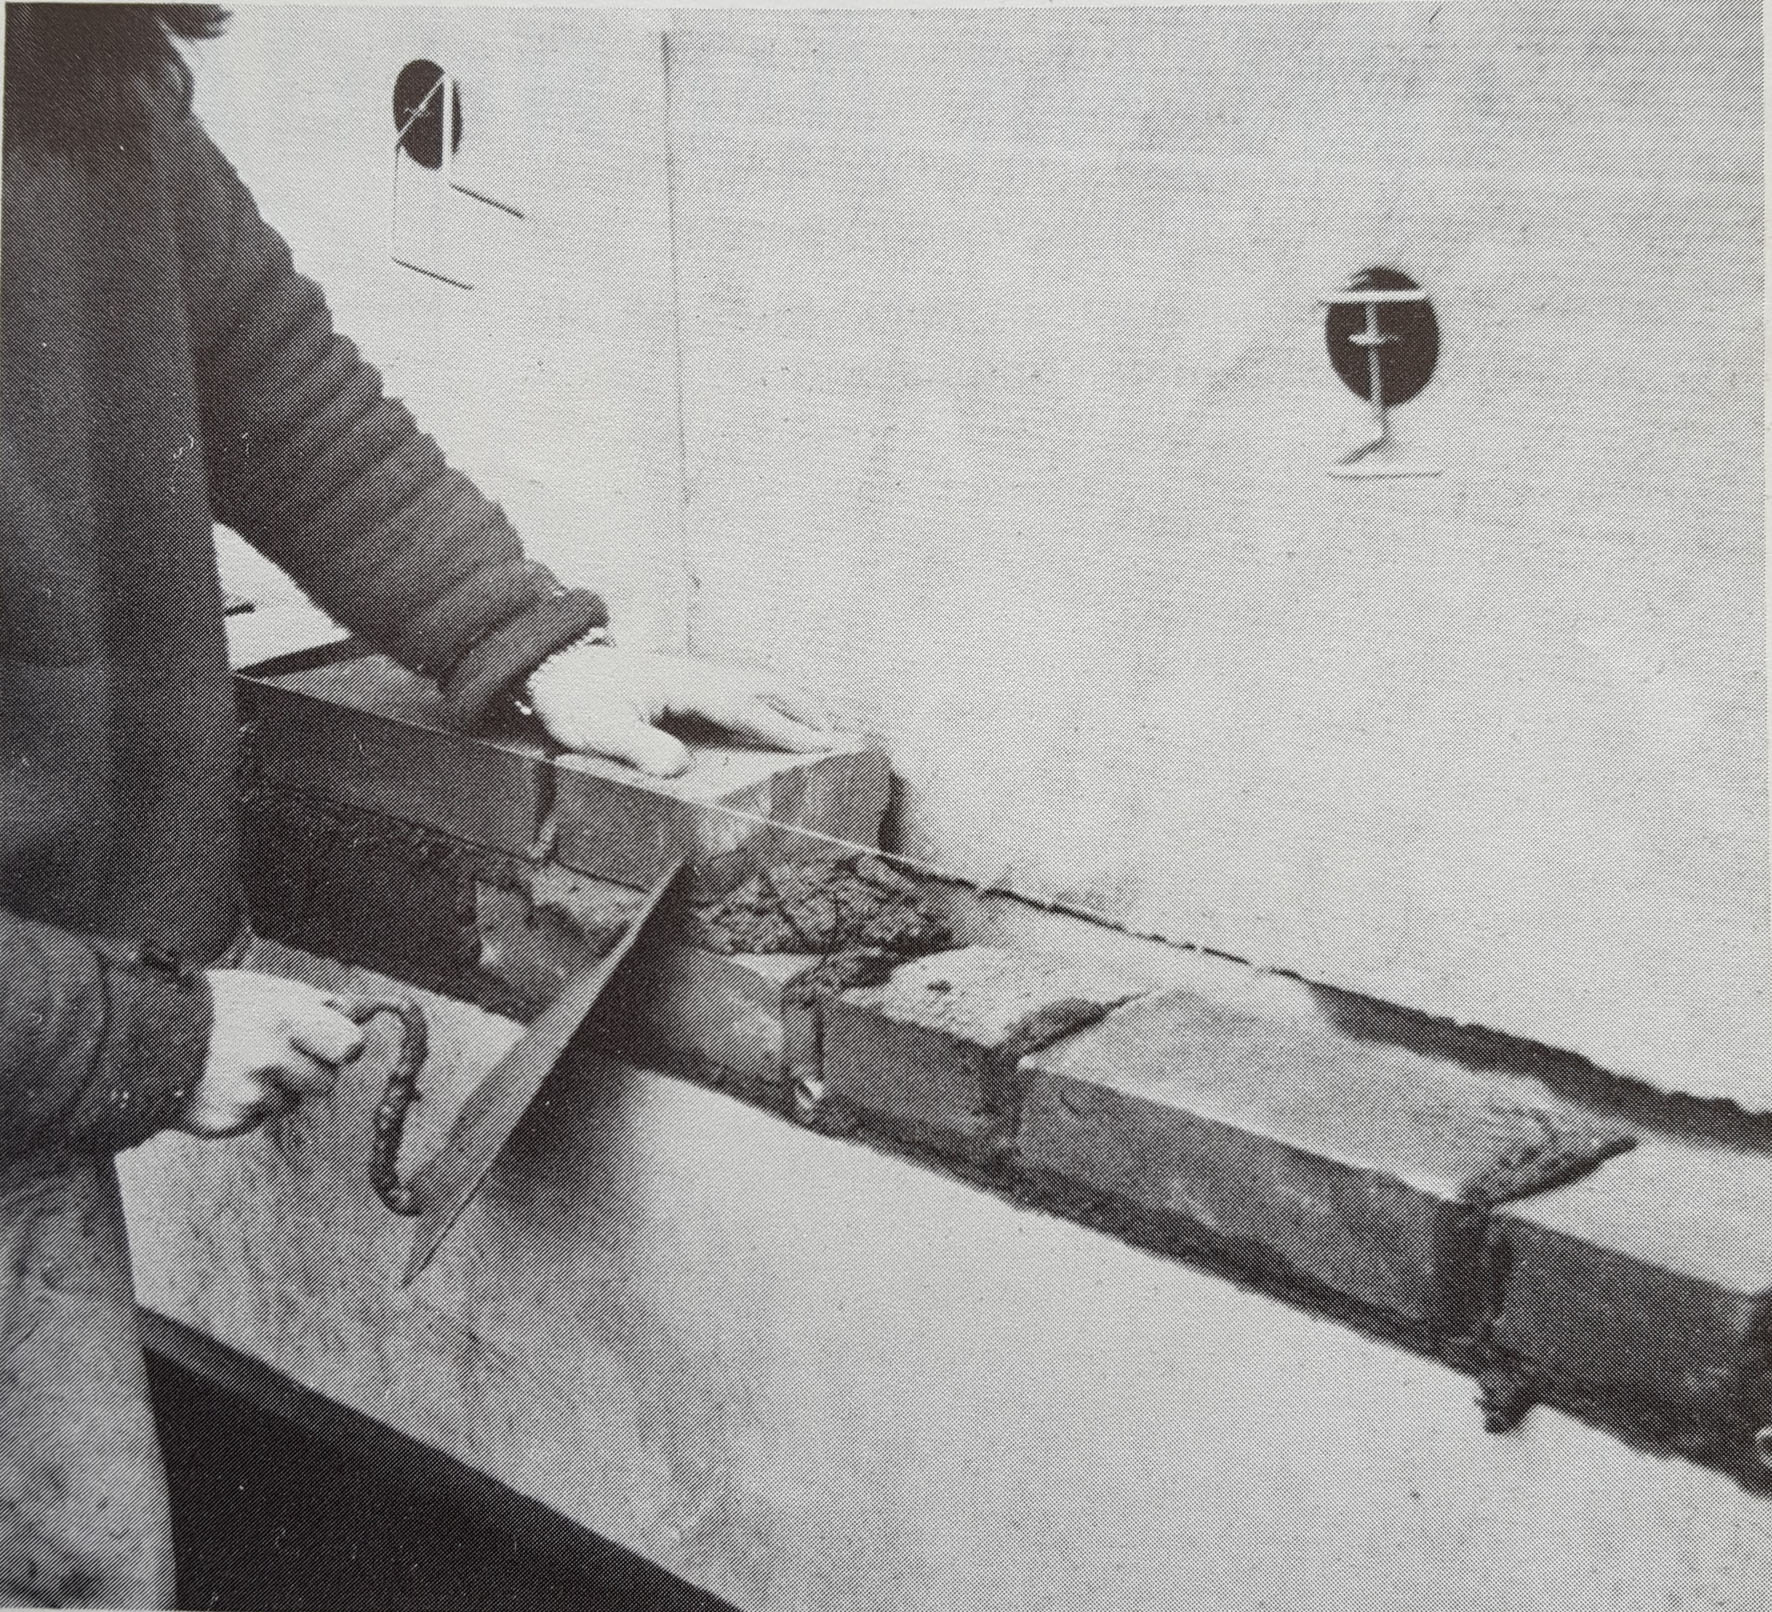
\includegraphics[width=0.8\linewidth ]{figure/Theory/brickLay.jpg}
\caption{The length of the curve is the same regardless of coordinate system.}
\end{figure}

There have not been many alternatives to this quite traditional way of making bricklaying. Methods have been made to combine concrete elements with bricks or using brick laying robots. These techniques give some possibilities that might be hard to achieve using traditional methods. A big difference is that you often get a industrial feeling, meaning perfect results, and you loose the human touch.

\begin{figure}[H]
\centering
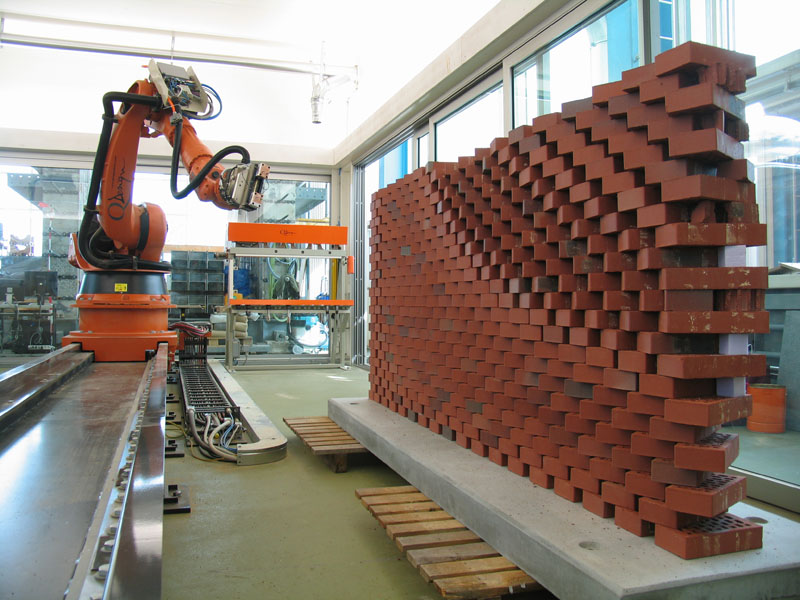
\includegraphics[width=0.9\linewidth ]{figure/Introduction/RobotBrick.jpg}
\caption{ETH Brick Robot}
\end{figure}



\subsection{Production and Realization}
\begin{figure}[H]
\centering
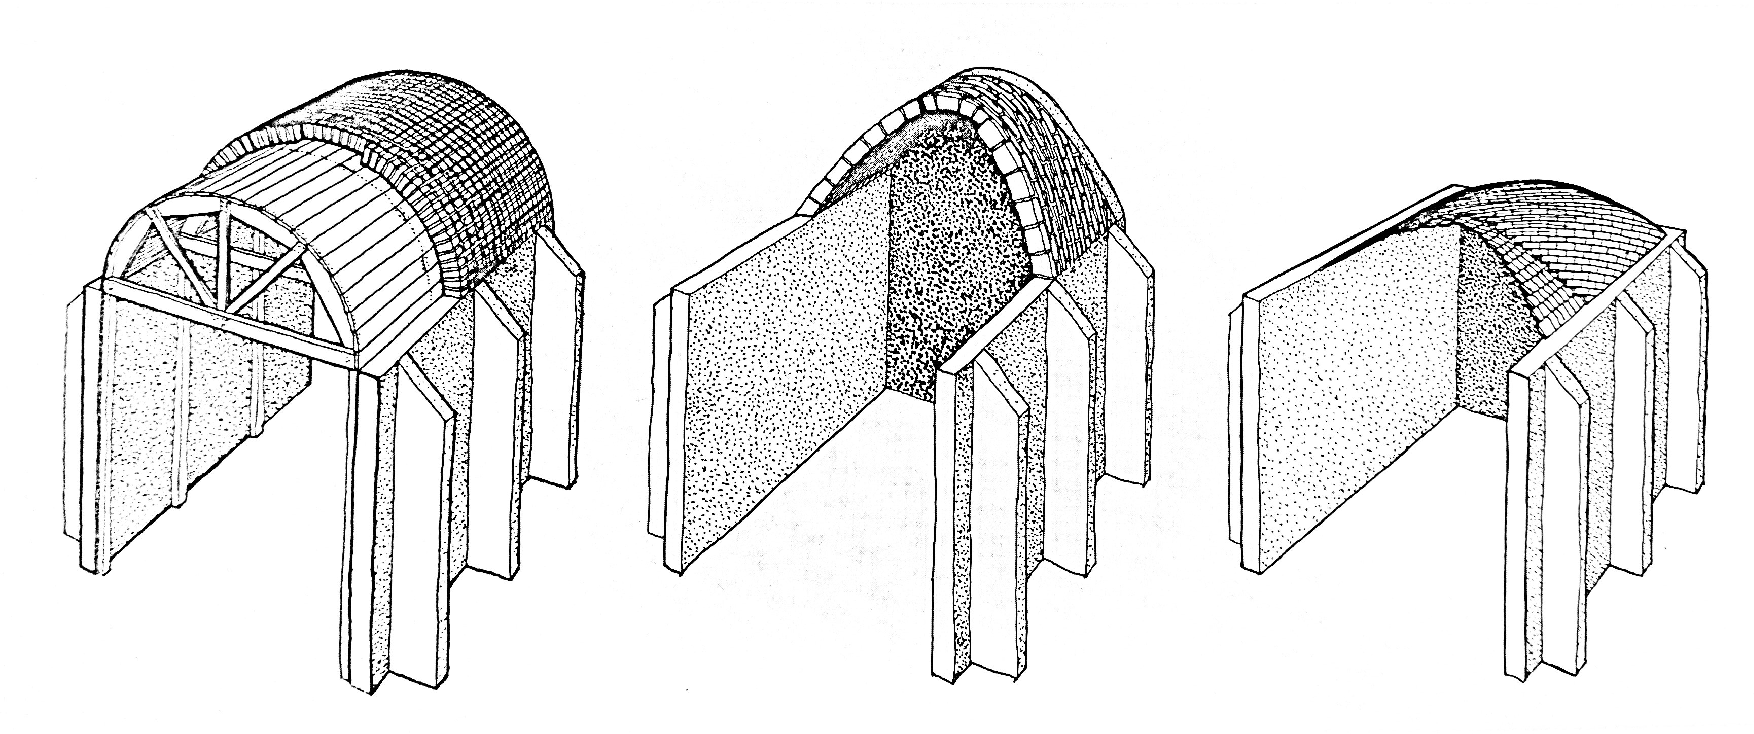
\includegraphics[width=0.9\linewidth ]{figure/Introduction/vaulting2.pdf}
\caption{The three main types vaulting}
\end{figure}

"Historically, masonry vaulting developed along three paths: the European, the Middle Eastern, and the Catalan (fig. 67) . The European path included Roman, Romanesque, Gothic, and Renaissance vaulting. The design of European vaults was generally based on the geometry of the circle, and the vaults were erected over temporary centering or form work. Working in this fashion resulted in relatively thick vaults, with the long dimensions of their stones or bricks lying along radial lines. The inclined thrusts of the vaults are resisted by either engaged or flying buttresses. 
The second path of development took place in the Middle East, where both barrel vaults and domes were erected without the use of centering. For vaults, centering was eliminated by inclining the courses of bricks against an end wall and for domes, by building in a spiral pattern. The resulting vault shapes often tended toward a parabolic geometry rather than a circular one, probably because it was easier for the mason, when working without centering, to keep bricks in place in a partially completed vault if they were laid along a parabolic line. Middle Eastern vaults are about as thick as European ones. Their thrusts are resisted by thick walls or engaged buttresses.
The third path of traditional masonry vault development— the Catalan vaulting technique— emerged in the region around Barcelona and is distinctly different from the other two. It utilizes multiple, overlapping laminations of thin tiles whose long dimensions lie in the curving surface of the vault. Catalan vaults are much thinner and lighter in weight than either European or Middle Eastern vaults. They are often also much shallower, sometimes rising as little as 10 percent of the span. They are extremely strong due to the staggering of joints between one tile lamination and the next. They are sometimes called timbrel vaults in reference to their extreme thinness, which is likened to that of the head of a timbrel, a small handdrum or tambourine."



\begin{figure}[H]
\centering
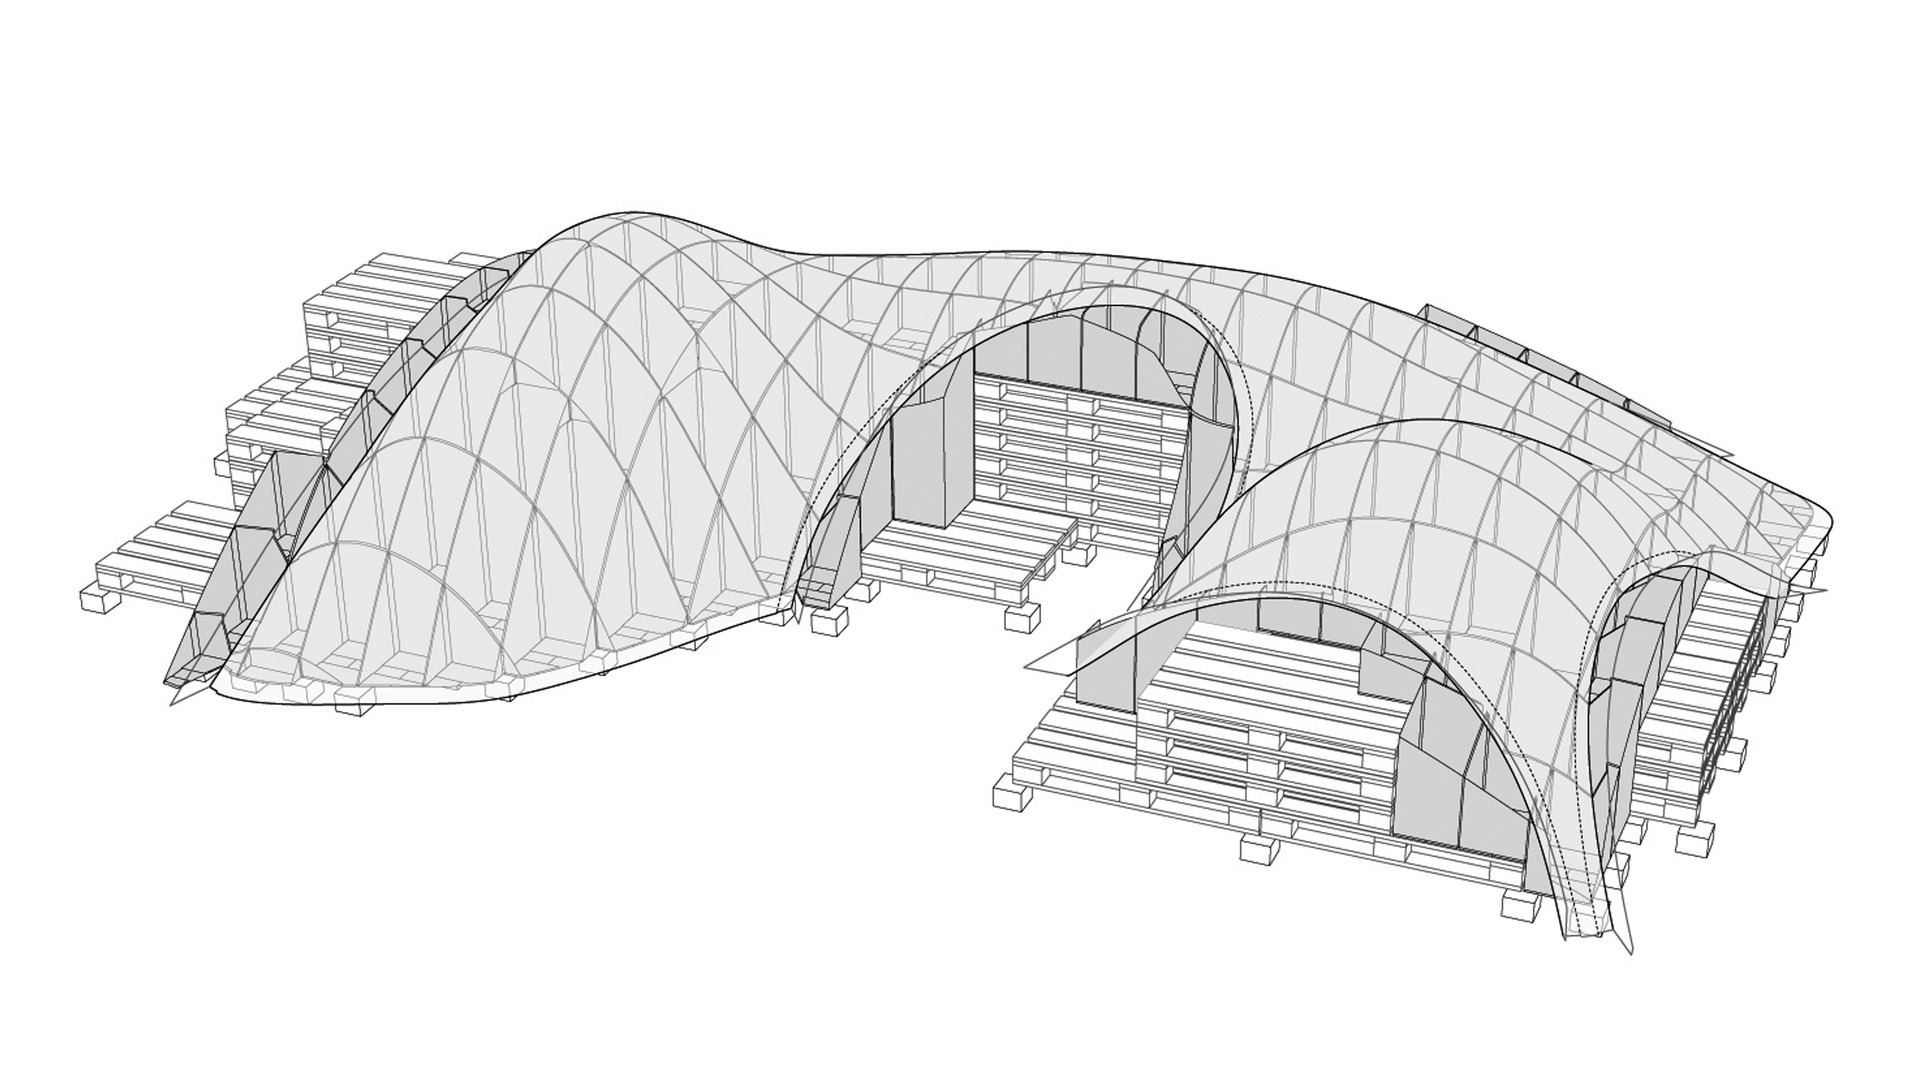
\includegraphics[width=0.45\linewidth ]{figure/Introduction/VaultBlock2.jpg}
\includegraphics[width=0.45\linewidth ]{figure/Introduction/VaultBlock.jpg}

\caption{The length of the curve is the same regardless of coordinate system.}
\end{figure}






\begin{figure}[H]
\centering
\includegraphics[width=0.9\linewidth ]{figure/Introduction/digitalstereotomyBlock.jpg}
\caption{Philippe Block}
\end{figure}

\begin{figure}[H]
\centering
\includegraphics[width=0.8\linewidth ]{figure/Introduction/digitalstereotomyBlock2.jpg}
\caption{Philippe Block}
\end{figure}


\subsection{Finding forms of equilibrium}

"As part of the conceptual design of structures, especially domes, shells and membrane structures, generating adequate structural shape is crucial to the load-bearing behaviour and aesthetic  expression of design.Their shapes cannot be freely chosen and conceived directly, due to the intrinsic interaction between form and forces. For such a problem one needs \textit{form finding}. Typical structures that require form finding include:" p 60 shells structures

\begin{itemize}
\item soap films within a given boundary.
\item prestressed, or hanging fabric membranes.
\item prestressed, or hanging cable nets.
\item structures generated by pressure.
\end{itemize}

The process of designing form-found shapes is called form finding or shape finding, the the former term

"Form-Finding is a forward process in which parameters are explicitely/directly controlled to find an 'optimal' geometry of structure which is in static equilibrium with a design loading "

The parameters that can be imposed to control the form-finding process are:

\begin{itemize}
\item \textit{Boundary Conditions}, which implies the supports and external loads.
\item \textit{Topology and Geometry}, what is the inital geometry and how are all members connected.
\item \textit{Internal forces}, 
\end{itemize}


\subsubsection{Graphical Methods}




\begin{figure}[H]
\centering
\includegraphics[width=0.6\linewidth ]{figure/Theory/graphStatEx.JPG}
\caption{Compression-only Form finding through Finite Subdivision of the
Force Polygon }
\end{figure}


\subsubsection{Analytical Methods}

For some cases is possible to analytically derive the shapes of funicular arches and shells, i.e only axial forces. It is not very common since it easily gets very complicated applying it to complex demands on a structure, both architectural and structural. For simple arches and shell it is though possible by assuming for instance constant loading,internal forces or stresses.  Chris Williams describes in the book \textit{Shell Structures for Architecture} how to attain the mathematical expressions for both arches and shells, with varying constraints.
You might also read \textit{ Tensile Structures Volume 2,  Cable nets} by Frei Otto for a descriptive way to analytically describe single cables and cable nets analytically. 

\begin{figure}[H]
\centering
\includegraphics[width=0.6\linewidth ]{figure/Introduction/constantShell.pdf}
\caption{Constant stress shells of derived analytically by Chris Willams. }
\end{figure}


\subsubsection{Physical methods}

"Designers of structures have used small-scale models when it is beneficial to do so, especially in order to raise the engineers confidence in the design being proposed. This may have been for many reasons. For example:" p 34 Shells structures

\begin{itemize}
\item The available calculation methods were to complex or time-consuming
\item it would be too costly to build a full-size prototype
\item it was believed that normal structural analysis methods would not adequately model the structure.
\item the geometry of the structure could not be defined using a mathematical equation
\item there were no other means available
\end{itemize}


Many have seen the the hanging cable models of \textit{Gaudi} but the  modern pioneer in this field was structural engineer and architect \textit{Frei Otto}. During the 20th century he elaborated with physical models to understand the shapes and design of light weight structures.

\begin{figure}[H]
\centering
\includegraphics[width=0.6\linewidth ]{figure/Theory/Soap.jpg}
\caption{The tangent differs depending of which direction you refer to. }
\end{figure}

\begin{figure}[H]
\centering
\includegraphics[width=0.6\linewidth ]{figure/Theory/Multihalle.jpg}
\caption{The tangent differs depending of which direction you refer to. }
\end{figure}



\subsubsection{Numerical Methods}


Computational Form-Finding algorithms can be divided in the following three branches according to Veenendal and Block. 

\begin{itemize}
\item Stiffness Matrix Methods
\item Geometric Stiffness Methods
\item Dynamic Equilibrium Methods 
\end{itemize}

\begin{figure}[H]
\centering
\includegraphics[width=0.6\linewidth ]{figure/Theory/PartSpring.jpg}
\caption{The tangent differs depending of which direction you refer to. }
\end{figure}


\subsection{Computational Design in Architecture}

Design in architecture often refers to creative design process where you explore different options related to specific task or conditions. The term "Thinking outside the box" is somewhat positive in the modern architecture in aspiration of new architecture. Computers on the other hand are bound to think inside the box based on logic rules.Though they are much more efficient in handling data and calculations then we humans do. Computational design can be seen as the merge of these two design concepts, thinking outside the box inside the box. The combination makes it possible to solve difficult problems that demands huge computational power or generate designs hard to imagine beforehand. 

Offices  that was early in defining units specialized in computational design and complex problem are \textit{Foster and Partners},\textit{ Arup} and \textit{Buro Happold}. Today there are more offices and academic institutes that specializes in this area.

\begin{figure}[H]
\centering
\includegraphics[width=0.9\linewidth ]{figure/Introduction/ICD.jpg}
\caption{Research pavilion 2011 designed by the Institute of Computational Design (ICD) }
\end{figure}

\subsubsection{Parametric Design}
Parametric Design is relatively new concept in Architecture that has been developed during the late 20th century and beginning of 21th century, and the development continues. 

"In parametric design it is the parameters of a particular design that are declared and not its shape. By assigning different values to the parameters, different objects or configurations can be created." Smart geometry
It is a way of seeing the design process as a rule-based system, which can be refereed as \textit{algorithmic thinking}."Algorithmic thinking allows designers  to rationalize, control, iterate, analyze and search for solutions in a defined solution space." Parametric Design for Architecture.
Examples of environments using a parametric concept is \textit{Grasshopper3d}, \textit{Dynamo} and 
\textit{Generative Components}.

\subsubsection{Design Scheme}

\begin{figure}[H]
\centering
\includegraphics[width=1.0\linewidth ]{figure/Introduction/DesignScheme.pdf}
\caption{The tangent differs depending of which direction you refer to. }
\end{figure}



\section{Purpose} 
\section{Limitations} \label{Section_ref}


